\documentclass[
	10pt, % Default font size, select one of 10pt, 11pt or 12pt
	fleqn, % Left align equations
	a4paper, %a4paper, b5paper
]{LegrandOrangeBook}

% Book information for PDF metadata, remove/comment this block if not required 
\hypersetup{
	pdftitle={Title}, % Title field
	pdfauthor={Author}, % Author field
	pdfsubject={Subject}, % Subject field
	pdfkeywords={Keyword1, Keyword2, ...}, % Keywords
	pdfcreator={LaTeX}, % Content creator field
}

\DeclareUnicodeCharacter{0301}{*************************************}

% Bibliography files
\addbibresource{refs.bib}

\definecolor{ocre}{RGB}{40, 173, 213} % Define the color used for highlighting throughout the book
\definecolor{part_title}{RGB}{29, 117, 175} % Define the color used for the title of parts
%\definecolor{part_title}{RGB}{45, 95, 144} % Define the color used for the title of parts

\chapterimage{} % Chapter heading image
\chapterspaceabove{6.5cm} % Default whitespace from the top of the page to the chapter title on chapter pages
\chapterspacebelow{6.75cm} % Default amount of vertical whitespace from the top margin to the start of the text on chapter pages

%----------------------------------------------------------------------------------------

\usepackage{siunitx}
\usepackage[capitalise, nameinlink]{cleveref}
\usepackage{float}
\usepackage{physics}
\usepackage{arydshln}
\usepackage{esint}

\usepackage{subfigure}
\usepackage{caption}

%% My commands %%
\newcommand{\dif}{\mathrm{d}}
\newcommand{\avg}[1]{\left<#1\right>}
\newcommand{\parentesi}[1]{\left(#1\right)}
\newcommand{\claudator}[1]{\left[#1\right]}
\newcommand{\keys}[1]{\left\{#1\right\}}
\newcommand{\limitss}[2]{_{#1}^{#2}}
\newcommand{\dpart}[2]{\frac{\partial #1}{\partial #2}}
\newcommand{\der}[2]{\frac{\dif #1}{\dif #2}}

\begin{document}

%----------------------------------------------------------------------------------------
%	COVER PAGE
%----------------------------------------------------------------------------------------

\begin{titlepage}
    %\pdfbookmark[1]{\myTitle}{titlepage}
    % if you want the titlepage to be centered, uncomment and fine-tune the line below (KOMA classes environment)
    	\large

        \begin{center}
            \sffamily
            
\includegraphics[width=.35\textwidth]{Figs/uib.png}
        
            \vspace*{.05\textheight}

			{\Huge\bfseries DOCTORAL THESIS} \\
			{\Large \bfseries 2024}

            \vspace*{.15\textheight}

			\begingroup
				{\Huge\bfseries Theoretical and data-driven models in Ecology \par}
			\endgroup

            \vfill

            {\Large \bfseries Àlex Giménez Romero}
        \end{center}
\end{titlepage}

%----------------------------------------------------------------------------------------
%	TITLE PAGE
%----------------------------------------------------------------------------------------

\thispagestyle{empty}

\begin{titlepage}
    %\pdfbookmark[1]{\myTitle}{titlepage}
    % if you want the titlepage to be centered, uncomment and fine-tune the line below (KOMA classes environment)
    \large

    \hfill
    \begin{minipage}[c][0.2\textheight]{0.45\textwidth}
        
\includegraphics[width=.75\textwidth]{Figs/uib.png}
    \end{minipage}
    \hfill
    \begin{minipage}[c][0.2\textheight]{0.45\textwidth}
        
\includegraphics[width=1\textwidth]{Figs/ifisc.pdf}
    \end{minipage}
    \hfill
    {\centering\sffamily
    \vspace*{.1\textheight}

    {\Huge\bfseries DOCTORAL THESIS} \\
    {\Huge\bfseries 2024}

    \bigskip

    {\Large\bfseries Doctoral programme in Physics} \\

    \vfill

    \begingroup
    {\Huge\bfseries Theoretical and data-driven models in Ecology \par}
    \endgroup

    \bigskip

    {\Large\bfseries Àlex Giménez Romero}

    \vfill
    }

    \begin{flushleft}
        \sffamily
        \textbf{Thesis Supervisor:} Manuel A. Matías \\
        \textbf{Thesis Tutor:} Crist\'obal L\'opez S\'anchez\\

        \vfill

        Doctor by the Universitat de les Illes Balears \\
    \end{flushleft}
\end{titlepage}

%----------------------------------------------------------------------------------------
%	COPYRIGHT PAGE
%----------------------------------------------------------------------------------------

\thispagestyle{empty} % Suppress headers and footers on this page

~\vfill % Push the text down to the bottom of the page
\sffamily

\noindent \textbf{Supervisors:}

\noindent Manuel Matías \\

\noindent Àlex Giménez Romero.

\noindent \textit{Theoretical and data-driven models in Ecology.} \copyright

\noindent Palma de Mallorca, July 2024
\pagebreak

%----------------------------------------------------------------------------------------
%	DEDICATION
%----------------------------------------------------------------------------------------
\thispagestyle{empty}

\vfill

\begin{center}
    \sffamily
    A en Manuel Miranda\\
    pel seu suport i ajuda\\
    durant tots aquests anys.\\
    Sempre estaràs amb mi.\\
    i recordare sempre\\
    el que em vas ensenyar.\\

\end{center}

\vfill
\newpage
\thispagestyle{plain} % empty
\mbox{}

%----------------------------------------------------------------------------------------
%	INTERNATIONAL PhD PROGRAM IN PHYSICS
%----------------------------------------------------------------------------------------

\newpage
\thispagestyle{plain} % empty
\mbox{}
\thispagestyle{empty}

Dr Manuel A. Matías of the Consejo Superior de Investigaciones
Cient\'ificas (CSIC)

\vspace*{2 cm}

I DECLARE:

\vspace*{1 cm}

That the thesis title \textit{Theoretical and data-driven models in Ecology},
presented by Àlex Giménez Romero to obtain a doctoral degree, has been
completed under my supervision.

\vspace*{2 cm}

For all intents and purposes, I hereby sign this document.

\vspace*{2 cm}

Signature

\vspace*{3 cm}

Dr. Manuel A. Matías

\vspace*{0.1 cm}

Thesis Supervisor

\vspace*{1 cm}

Palma de Mallorca, July 2024

\vfill
\newpage
\thispagestyle{plain} % empty
\mbox{}

%----------------------------------------------------------------------------------------
%	ACKNOWLEDGEMENTS
%----------------------------------------------------------------------------------------

\begin{center}
    \textbf{\Large Agraïments}
\end{center}

{
\parindent=0pt

Aquesta tesi no hauria estat possible sense l'ajuda de moltes persones, així
que aquesta secció també serà llarga. \\

% Manuel
En primer lloc, la persona que més ha contribuit a aquest treball és el meu
director, el Dr. Manuel Matías. És gracies a ell que he tingut l'oportunitat de
realitzar aquesta tesi i començar la meva carrera investigadora. Li estic
especialment agraït per confiar en mi des del primer moment, quan el meu
historial acadèmic no era el més prometedor. També li estic agraït per la forma
en què m'ha \textbf{guiat} durant tot el procés i tot el que m'ha ensenyat,
tant en l'àmbit acadèmic com en el personal. Tinc clar que, per mi, es el
millor director que hauria pogut tenir. \\

% Colaboradors articles
Els meus colaboradors també mereixen un agraïment especial. Primer de tot vull
agrair a l'Iris Hendriks, qui va ser la primera persona amb qui vaig començar a
colaborar, ja durant el meu TFM, i Amalia Grau. Juntament amb el meu director,
conformen els coautors del meu primer article sobre l'esdeveniment de
mortalitat massiva de les nacres. Aquest treball va ser el punt de partida de
la meva tesi i va ser possible gràcies a la seva ajuda. Una menció a en
Cristóbal López i en Federico Vazquez (a.k.a Fede), amb qui vam continuar
treballant en aquest tema. Seguim amb Eduardo Moralejo, coautor de la majoria
d'articles presents en aquesta tesi, qui em va endinsar en el món de la
fitopatologia i amb qui vaig començar a treballar en el projecte de la
\textit{Xylella fastidiosa}. Espero que aquesta col·laboració segueixi en el
futur. En relació amb aquest mateix tema, també vull esmentar la Clara Lago,
Arantzazu Moreno i Alberto Fereres, amb qui he tingut l'oportunitat de
col·laborar. Els estic especialment agraïts per ``acollir-me'' durant el
congrés que organitzaven a Madrid. També agrair aquí a un científic ``de la
casa'', Jose Ramasco, no només per la part purament científica, sinó també per
les converses que hem tingut. Probablement és de les persones més ocupades del
IFISC, però també de les més maques. Per acabar amb aquest tema vull agrair a
Jose Gutiérrez i Maialen Iturbide, qui em van acollir durant la meva estada a
Santander. No tinc paraules per expressar la meva gratitud per la seva
amabilitat, incloent que m'oferissin el seu cotxe per visitar la zona! Va ser
una experiència molt enriquidora i espero que puguem seguir col·laborant en el
futur. Un agraïment també a la Susana Flecha, amb qui vam tenir una
col·laboració molt fructífera. Va ser un plaer treballar amb ella i espero que
puguem seguir treballant junts. També vull agrair a en Tomas Sintes, amb qui he
tingut reunions i viatges molt divertits. Sempre recordaré el viatje a Arabia
Saudita, amb en Manuel, l'Eva i en Miguel. Cal dir que es l'unic professor amb
qui he compartit un llit! Ha estat un plaer treballar amb ell i espero que
puguem seguir col·laborant en el futur. Finalment un agraïment especial a en
Carlos Duarte, amb qui he tingut l'oportunitat de col·laborar en un projecte
molt interessant sobre coralls. Primer de tot, agrair la seva invitació a
Arabia Saudita, que com ja he dit va ser una experiència molt
enriquidora i divertida. També agrair-li per la seva ajuda i el coneixement que
m'ha transmès, encara que sigui de forma inconscient. Espero que aquesta
col·laboració segueixi en el futur. \\

% Altres col·laboradors
També vull agrair alguns col·laboradors que no han estat coautors dels articles
d'aquesta tesi, però que han contribuit de forma significativa. Primer de tot
vull agrair a en Dan Bebber, amb qui vaig tenir l'oportunitat de treballar
durant un mes en remot. També una menció especial a en Rob Salguero, amb qui
vaig tenir el plaer de treballar durant 3 mesos en una estada al departament de
biologia de la universitat d'Oxford. Va ser una experiència molt enriquidora
poder veure com es treballa en un entorn tan diferent al de l'IFISC. Aquests
tres mesos van ser també molt fructífers i vaig aprendre moltíssim. Va ser un
plaer treballar amb ell i espero que puguem seguir col·laborant en el futur.
També vull agrair a en Pere Colet i la Rosa López, amb qui he tingut
l'oportunitat de donar classes. Han confiat en mi tant per donar classes de
grau com de màster i els estic molt agraït per això. \\

% IFISC
Un agraïment especial a tots els membres de l'IFISC i la UIB. En primer lloc,
a l'equip de neteja, invisibles però imprescindibles. En especial a l'Anna
Pérez, amb qui coincidia gairebé cada matí, ben d'hora. També agrair els
membres de l'administració per la seva ajuda en tot moment, sobretot a la Marta
Ozonas, l'Inma Carbonell, la Neus Lacomba, la Maria Quetglas i l'Alberto
Sánchez. També agrair a l'Adrián García tota la seva ajuda en la part de
divulgació científica. Sense ell tot el que hem fet en aquest aspecte no hauria
estat possible. Finalment, un agraiment més que especial als técnics (i
ex-técnic) de l'IFISC: l'Eduard Solivelles, l'Antònia Tugores i en Rubén
Tolosa. Literalment, sense ells aquesta tesi (i totes les de l'IFISC) no
haurien estat posibles. Els estic molt agraït per tota la seva ajuda, les seves
explicacions i la seva paciència, a més d'altres conversacions més
``informals''. \\

% Amics
També vull agrair a tots els meus amics i companys del IFISC, que han estat una
part molt important de la meva vida durant aquests anys. M'agradaría començar
amb els que fa més temps que conec. El primer lloc indiscutible l'ocupa l'Adrià
Labay (a.k.a DJ Labay), amb qui vaig començar la carrera de Física a la UAB,
amb qui casi morim al Monte Perdido (i a les festes de Martorell, les colònies
o Dresden) i sense qui, probablement, no hauria acabat la carrera. Els següents
a la llista son en David, Miguel, los canarios (Javi Galvan \& Medi) i Jogito,
qui conec des del máster. Amb ells he compartit rutillas, festes, molts
exercisis i entregues i, sobretot, moltes rialles. Una menció especial a en
David, qui també va ser un vei i un usuari del camelecar, i ha estat una ajuda
imprescindible en la part d'escritura d'aquesta tesi: gracies per anar dues
setmanes adelantat. També per en Miguel, amb qui he tingut converses molt
interessants i de qui admiro la seva curiositat i ganes de seguir aprenent (i
la locura de entrecot que nos hizo en su casa). Seguim amb els que vaig
coneixer entre el máster i el començament del doctorat: Pablo, Irene, Maria,
Javi Aguilar, Medea, Rodri i Mou (o Mou i Rodri). Ells em van acollir quan vaig
arribar per fer el doctorat i es van encarregar de fer la vida post-pandèmia
més fàcil i divertida. En Pablo, la Irene i la Maria mereixen una menció
especial per acompanyar-me en les meves rutes chill i no tan chill, a Sabotage
i en general aquests anys. El següent grup el formen els increibles companys i
fundadors de ZULO: Mar Ferri, Fer (desertor, pero tt gym), Mar Cuevas, Gorka,
Guillem, Pau i Manuel Miranda. Aquests 10 metres quadrats sense llum natural ni
ventilació haurien estat insuportables sense vosaltres. Aqui també agrair les
noves incorporacions, com en Jaume, la Sara o en Coque. Finalment tenim alguns
dels integrants de la S07: Jesus, Bea, Lisa, Pepe, Dimitris i Daniele. Una
menció especial a Jesus i Bea, per haver compartit mes temps amb mi i, en
conseqüència, haver aguantat més chapes i gaudit de més barbacoas amb tremendo
allioli. També voldria agrair als postdocs amb qui hem comparitit dinars i
alres moments, sobretor l'Eva. Finalment, vull tornar a agrair en Manuel
Matías, a qui també considero un amic. Espero que, a part de seguir
col·laborant, puguem seguir compartint sopars i copes de vi. \\

% Barri, Carmela, família
Per acabar, vull agrair als meus amics de Barcelona, especialment a la Lidia,
l'Alex Jimenez i el Guti. Fora de l'ambit acadèmic, son els amics que més han
escoltat tant els meus exits i avanços com les meves queixes, frustracions i
fracassos. També agrair a la Carmela, que ha estat una part molt important de
la meva vida durant aquests anys. Ella es l'única persona que ha estat al meu
costat les 24 hores del dia, 7 dies a la setmana, 365 dies a l'any. Sense ella
segurament hauria acabat aquesta tesi, pero probablement també hauria acabat
amb la meva salut mental. Tinc molta sort de tenir-la al meu costat, des de
Barcelona, a Mallorca, a Oxford i properament a Blanes; a tot arreu on de
moment m'ha seguit. Li estic especialment agraït. També he de dir que si no fos
per ella moltes figures d'aquesta tesi serien apreciablement més lletges...
Finalment vull agrair a la meva família per haver-me donat l'oportunitat de
formar-me i per haver-me donat suport en tot moment.
}

\vfill
\newpage
\thispagestyle{plain} % empty
\mbox{}

%----------------------------------------------------------------------------------------
%	RESUM
%----------------------------------------------------------------------------------------

\pagebreak
\thispagestyle{empty}

\begin{center}
    \textbf{\Large Resum}
\end{center}

La vida a la Terra ha evolucionat al llarg de milions d'anys,
produint una rica diversitat d'espècies i ecosistemes que proporcionen serveis
essencials per a la supervivència humana. No obstant això, aquesta
biodiversitat està disminuint ràpidament a causa d'activitats humanes
com la destrucció d'hàbitats, el canvi climàtic, les espècies invasores i les
malalties emergents. Aquests factors interconnectats estan provocant una pèrdua
generalitzada d'espècies i la ràpida degradació dels ecosistemes, cosa que
amenaça l'estabilitat ecològica global i la prosperitat humana. Per abordar
aquesta crisi es requereix un enfocament interdisciplinari que permeti
comprendre i mitigar els seus impactes, assegurant la preservació de la
biodiversitat i la sostenibilitat de les societats humanes.

En aquesta tesi desenvolupem mètodes teòrics i basats en dades per estudiar
problemes relacionats amb la pèrdua de biodiversitat causada pel canvi
climàtic i les malalties emergents. A través de la lent dels sistemes
complexos, abordem desafiaments contemporanis com la propagació de malalties,
l'acidificació dels oceans i el declivi d'ecosistemes crítics com els esculls
de corall o les praderies marines de \textit{Posidonia oceanica}. Ens basem en
una combinació de models matemàtics, simulacions computacionals i tècniques
avançades d'anàlisi de dades per obtenir una comprensió més profunda daquests
complexos fenòmens ecològics.

A les dues primeres parts d'aquesta tesi, desenvolupem models matemàtics
per avançar la nostra comprensió sobre les dinàmiques de transmissió de
malalties marines i transmeses per vectors. Ens centrem en dos exemples:
l'Esdeveniment de Mortalitat Masiva (MME) de \textit{Pinna nobilis} i les
malalties de plantes causades pel bacteri \textit{Xylella fastidiosa}.
Investiguem el paper de factors clau com la temperatura o la mobilitat de
patògens a la transmissió de l'MME i l'impacte de l'abundància estacional
d'insectes vectors a la propagació de malalties de plantes. Aquests models
proporcionen noves perspectives sobre els mecanismes que faciliten aquestes
malalties aixi com sobre el seu control i maneig.

A la tercera part, apliquem aquest coneixement adquirit per desenvolupar un
nou marc teòric per predir la distribució potencial de malalties de
plantes transmeses per vectors en funció de factors ambientals i
climàtics. Demostrem la utilitat d'aquest model en predir el risc de la
malaltia de Pierce de la vinya, causada per \textit{Xylella fastidiosa}, en
escenaris climàtics actuals i futurs. La nostra metodologia representa un
avenç significatiu en el camp de la biogeografia de malalties, ja que
proporciona una forma d'integrar les interaccions ecològiques complexes
inherents a les malalties per predir el seu possible establiment a
funció de les condicions ambientals.

Finalment desenvolupem i apliquem mètodes basats en dades per monitoritzar i
avaluar la salut dels ecosistemes marins costaners. Utilitzant tècniques
d'aprenentatge profund, presentem un marc innovador per reconstruir sèries
temporals de pH oceànic incompletes, millorant la nostra capacitat de
monitoritzar la acidificació oceànica amb precisió. A més, fem servir
aprenentatge automàtic i imatges satel·litàries per mapejar i avaluar l'estat
de les praderies marines de \textit{Posidonia oceanica}, oferint un enfocament
escalable i rendible per a la monitorització d'aquests ecosistemes. Finalment
fem una anàlisi global de les propietats espacials dels esculls de corall
utilitzant dades de teledetecció, descobrint patrons universals en la
distribució de la mida i la geometria dels esculls.

Aquesta tesi subratlla la importància de la investigació interdisciplinària,
integrant la teoria ecològica, la ciència de sistemes complexos i la
intel·ligència artificial per abordar els desafiaments ecològics. Les troballes
contribueixen al desenvolupament d'estratègies de conservació efectives, amb
l'objectiu de mitigar els impactes del canvi climàtic i les malalties
emergents a la biodiversitat. En última instància, aquest treball recolza els
esforços per preservar la integritat dels ecosistemes i garantir la
sostenibilitat de les societats humanes davant dels canvis ambientals en
curs.

\vfill

%----------------------------------------------------------------------------------------
%	RESUMEN
%----------------------------------------------------------------------------------------

\begin{center}
    \textbf{\Large Resumen}
\end{center}

La vida en la Tierra ha evolucionado a lo largo de millones de años,
produciendo una rica diversidad de especies y ecosistemas que
son fundamentales para la supervivencia humana. Sin embargo, esta biodiversidad
está disminuyendo rápidamente debido a actividades humanas como la destrucción
de hábitats, el cambio climático, las especies invasoras y las enfermedades
emergentes. Estos factores interconectados están provocando una pérdida
generalizada de especies y la degradación acelerada de los ecosistemas, lo que
amenaza la estabilidad ecológica global y la prosperidad humana. Para abordar
esta crisis se requiere un enfoque interdisciplinario que permita comprender y
mitigar sus impactos, asegurando la preservación de la biodiversidad y la
sostenibilidad de las sociedades humanas.

En esta tesis desarrollamos métodos teóricos y basados en datos para estudiar
problemas relacionados con la pérdida de biodiversidad causada por el cambio
climático y las enfermedades emergentes. A través de la lente de los sistemas
complejos, abordamos desafíos contemporáneos como la propagación de
enfermedades, la acidificación de los océanos y el declive de ecosistemas
críticos como los arrecifes de coral o las praderas marinas. Nos basamos en una
combinación de modelos matemáticos, simulaciones computacionales y técnicas
avanzadas de análisis de datos para obtener una comprensión más profunda de
estos complejos fenómenos ecológicos.

En las dos primeras partes de esta tesis, desarrollamos modelos matemáticos
para avanzar nuestra comprensión de la dinámica de transmisión en enfermedades
marinas y transmitidas por vectores. Nos centramos en dos ejemplos: el Evento
de Mortalidad Masiva (MME) de \textit{Pinna nobilis} y las enfermedades de
plantas causadas por la bacteria \textit{Xylella fastidiosa} (Xf). Investigamos
el papel de factores clave como la temperatura o la movilidad de patógenos en
la transmisión del MME y el impacto de la estacionalidad en la abundancia de
vectores en la propagación de enfermedades de plantas. Estos modelos brindan
nuevas perspectivas sobre los mecanismos que facilitan estas enfermedades asi
como sobre su control y manejo.

En la tercera parte, aplicamos este conocimiento adquirido para desarrollar un
nuevo marco teórico para predecir la distribución potencial de enfermedades de
plantas transmitidas por vectores en función de factores climáticos.
Demostramos la utilidad de este modelo al predecir el riesgo de la
enfermedad de Pierce de la vid, causada por Xf, en escenarios climáticos
actuales y futuros. Nuestra metodología representa un avance significativo en
el campo de la biogeografía de enfermedades, permitiendo integrar las complejas
interacciones ecológicas inherentes a las enfermedades para predecir su posible
establecimiento en función de las condiciones ambientales.

Finalmente desarrollamos métodos basados en datos para monitorizar y
evaluar la salud de los ecosistemas marinos costeros. Utilizando técnicas de
aprendizaje profundo, presentamos un marco innovador para reconstruir series
temporales de pH oceánico incompletas, mejorando nuestra capacidad de
monitorizar la acidificación oceánica con precisión. Además, empleamos
aprendizaje automático e imágenes satelitales para mapear y evaluar el estado
de las praderas marinas de \textit{Posidonia oceanica}, ofreciendo un enfoque
escalable y rentable para monitorizar estos ecosistemas. Finalmente
realizamos un análisis global de las propiedades espaciales de los arrecifes de
coral utilizando datos de teledetección, descubriendo patrones universales en
la distribución del tamaño y la geometría de los arrecifes.

Esta tesis subraya la importancia de la investigación interdisciplinar,
integrando ecología, sistemas complejos e inteligencia artificial para abordar
los desafíos ecológicos. Los hallazgos contribuyen al desarrollo de estrategias
de conservación, con el objetivo de mitigar los impactos del cambio climático y
las enfermedades emergentes. Nuestro trabajo contribuye a
preservar la integridad de los ecosistemas y garantizar la sostenibilidad de
las sociedades humanas frente al cambio climático.

\vfill

%----------------------------------------------------------------------------------------
%	ABSTRACT
%----------------------------------------------------------------------------------------

\pagebreak
\thispagestyle{empty}

\begin{center}
    \textbf{\Large Abstract}
\end{center}

Life on Earth has evolved over billions of years, resulting in a rich
diversity of species and ecosystems that provide essential services for
human survival and well-being. However, this biodiversity is rapidly
declining due to human activities such as habitat destruction, climate
change, invasive species and emergent diseases. These interconnected
drivers are causing widespread loss of species and degradation of
ecosystems, threatening global ecological stability and human prosperity.
Addressing this crisis requires an interdisciplinary approach to understand
and mitigate its impacts, ensuring the preservation of biodiversity and the
sustainability of human societies.

In this thesis we develop theoretical and data-driven methods
to address pressing issues in Ecology and Conservation Biology through the
lens of Complex Systems and interdisciplinary research. We address a
range of contemporary challenges related to biodiversity loss driven by
climate change and emerging diseases. These challenges include the spread
of diseases, ocean acidification and the decline of critical ecosystems such as
coral reefs and seagrass meadows. We rely on a combination of theoretical
models, computational simulations, and advanced data analysis techniques to
gain a deeper understanding of these complex ecological phenomena.

In the first two parts of this thesis we develop mathematical models of
disease spread to fill knowledge gaps in the transmission dynamics of
marine and vector-borne plant diseases. We focus on two case studies: the
Mass Mortality Event (MME) of \textit{Pinna nobilis} and the vector-borne plant
diseases caused by the bacterium \textit{Xylella fastidiosa}. We investigate
the role of key factors such as temperature or pathogen mobility in the
transmission of the MME, and the impact of the non-periodic seasonal abundance
of insect vectors on the spread of plant diseases. These models provide
insights into the mechanisms driving the dynamics of these diseases, and the
potential for their control and management.

In the third part, we apply this gained knowledge to develop a novel
theoretical framework to predict the potential distribution of
vector-borne plant diseases based on environmental and climatic factors. We
demonstrate the utility of this model by predicting the risk of Pierce's
Disease of grapevines, caused by \textit{Xylella fastidiosa}, under current
and future climate scenarios. Our methodology represents a significant
advancement in the field of disease biogeography, providing a way to
integrate the inherent complex ecological interactions of diseases to predict
its potential establishment based on environmental conditions.

Finally, in the fourth part of this thesis, we develop and apply
data-driven methods to monitor and assess the health of coastal marine
ecosystems. We present an innovative framework to reconstruct missing data
from ocean pH time-series using deep learning techniques, which enhance our
ability to monitor ocean acidification accurately. Additionally, we employ
machine learning and satellite imagery to map and evaluate the condition of
seagrass meadows, offering a scalable and cost-effective approach to
ecosystem monitoring. Moreover, we conduct a global analysis of the spatial
properties of coral reefs using remote sensing data, uncovering universal
patterns in reef size distribution and geometry. These insights are crucial
for developing targeted conservation strategies to protect these vulnerable
ecosystems.

This thesis underscores the importance of interdisciplinary research,
integrating ecological theory, complex systems science, and artificial
intelligence to tackle ecological challenges. The findings contribute to
the development of effective conservation strategies, aiming to mitigate
the impacts of climate change and emergent diseases on biodiversity.
Ultimately, this work supports efforts to preserve the integrity of
ecosystems and ensure the sustainability of human societies in the face of
ongoing environmental changes.

\vfill

%----------------------------------------------------------------------------------------
%	TABLE OF CONTENTS
%----------------------------------------------------------------------------------------

\pagestyle{empty} % Disable headers and footers for the following pages

\tableofcontents % Output the table of contents

%\listoffigures % Output the list of figures, comment or remove this command if not required

%\listoftables % Output the list of tables, comment or remove this command if not required

\pagestyle{fancy} % Enable default headers and footers again

\cleardoublepage % Start the following content on a new page

%----------------------------------------------------------------------------------------
%	LIST OF PUBLICATIONS
%----------------------------------------------------------------------------------------

\chapterimage{} % Chapter heading image
\chapterspaceabove{6.75cm} % Whitespace from the top of the page to the chapter title on chapter pages
\chapterspacebelow{7.25cm} % Amount of vertical whitespace from the top margin to the start of the text on chapter pages

\chapter*{List of publications}

\begin{enumerate}
	\item \fullcite{GimenezRomero2021}
	      \vspace{0.5 cm}
	\item \fullcite{Flecha2022}
	      \vspace{0.5 cm}
	\item \fullcite{GimenezRomero_2022_RSos}
	      \vspace{0.5 cm}
	\item \fullcite{GimenezRomero2022_PRE}
	      \vspace{0.5 cm}
	\item \fullcite{GimenezRomero2022_CommsBio}
	      \vspace{0.5 cm}
	\item \fullcite{GimenezRomero2023}
	      \vspace{0.5 cm}
	\item \fullcite{GimenezRomero2023_PD}
	      \vspace{0.5 cm}
	\item \fullcite{GimenezRomero2024}
	      \vspace{0.5 cm}
	\item A comprehensive dataset on global coral reefs size and geometry
	\item Universal spatial properties of coral reefs
	\item Mapping the distribution of seagrass meadows from space with deep
	      convolutional neural networks
\end{enumerate}

\chapter*{Other publications}

\begin{enumerate}
	\item \fullcite{Lago2023}
	      \vspace{0.5 cm}
\end{enumerate}

%----------------------------------------------------------------------------------------
%	PART I: Introduction
%----------------------------------------------------------------------------------------

\part{Introduction}

%----------------------------------------------------------------------------------------
%	Introduction
%----------------------------------------------------------------------------------------
\chapterimage{biodiversity.jpg}
\chapterspaceabove{6.75cm}
\chapterspacebelow{7.25cm}

\chapter{The global biodiversity crisis}
\setcounter{page}{0}

\section{\label{sec:Introduction_1} Introduction}

%Initial paragraph about ecosystems and biodiversity
Based on our current understanding, life on Earth appears to be unique in the
Universe. Its existence is the result of a long evolutionary process that
started around 3.5 billion years ago \cite{Taylor_1993,Schopf2006},
producing a wide variety of life forms. From the simplest unicellular organisms
to the most complex multicellular forms, the diversity of life is so vast that
it is estimated that there are around 9 million species of living beings in our
planet \cite{Cardinale2012}. This biodiversity is the result of the interaction
among organisms and with their environment, which has led to the development of
complex ecosystems. Ecosystems are the basic units of life on Earth, where
organisms interact with each other and with the environment, forming a
self-regulating system that is capable of maintaining life \cite{Levin2005}.
As Simon Levin eloquently describes:

\begin{displayquote}
  ``\textit{Ecosystems and the biosphere are complex adaptive systems, in which
    pattern
    emerges from, and feeds back to affect, the actions of adaptive individual
    agents, and in which cooperation and multicellularity can develop and
    provide
    the regulation of local environments, and indeed impose regularity at
    higher
    levels. The history of the biosphere is a history of coevolution between
    organisms and their environments, across multiple scales of space, time,
    and
    complexity.}''
\end{displayquote}

% Paragraph on the importance of biodiversity -- ecosystem services
Besides its intrinsic value, biodiversity is essential for the proper
functioning of ecosystems \cite{Gamfeldt2008}, which in turn provide
fundamental services to humankind. These services, known as ecosystem services,
include the production of oxygen, the regulation of the climate, the provision
of food and water, and many others \cite{Daily1997}. Beyond these fundamental
life-supporting benefits, biodiversity also plays critical roles in nutrient
cycling and soil formation, processes integral to the sustainability of our
agricultural systems. The diversity of plant and animal life contributes to
robust ecosystems that can withstand and recover from a variety of disasters,
thereby ensuring ecological resilience. Moreover, biodiversity supports
recreational and tourism industries, which are significant sources of income
for many communities worldwide. The aesthetic and cultural values provided by
diverse ecosystems foster mental and physical health, and contribute to the
cultural heritage of communities, enriching our experience of the world.
Without services ecosystems provide, the stability of environments that support
human life would be greatly diminished, leading to profound economic and social
consequences.

% Paragraph on biodiversity loss, the biodiversity crisis
Unfortunately, the diversity of life on Earth is dramatically diminishing
\cite{Hughes1997,Ceballos2002,Pereira2010}, posing a serious threat to the
stability of ecosystems and the services they provide. Nowadays, wildlife
extinction rates are estimated to be 100 to 1000 times higher than the natural
background rate \cite{Ceballos2015,Pimm2014}, and up to 50\% of higher
taxonomic groups are already critically endangered \cite{Smith2009}. In the
last 50 years, the global population of vertebrates has declined by 69\%, about
50\% of the corals have disappeared due to different causes, mangroves
continue to be deforested at a rate of 0.13\% per year and roughly 10 million
hectares of forests are lost annualy \cite{WWF2022}. Sadly, I could continue
listing more examples of biodiversity loss, but the point is clear: we are
facing a global biodiversity crisis. Indeed, this has led some scientists to
propose that we are entering the sixth mass extinction event in Earth's history
\cite{Barnosky2011}. However, unlike the natural extinction events in Earth’s
past, the current crisis is precipitated by only one species: humans. As
ecosystems falter and species vanish, the intricate web of life that sustains
economies, food security, and our very existence is at risk. If left unchecked,
the repercussions of this biodiversity crisis may lead to ecosystems so
impaired that they no longer fulfill their roles, fundamentally altering the
living conditions on our planet.

% Paragraph on the drivers of biodiversity loss
The main drivers of global biodiversity loss, as identified in the Millennium
Ecosystem Assessment \cite{finlayson2005millennium}, encompass a range of
direct impacts on the natural world. Habitat change, exemplified by the rapid
deforestation in the Amazon Rainforest, results in drastic reductions in
biodiversity by stripping away the complex web of life supported by these
environments \cite{Laurance2012}. Climate change brings about shifts in
temperature and precipitation patterns that are markedly altering habitats, in
particular polar regions, threatening ice-dependent species with extinction
\cite{Post2013}. Indeed, climate change may be a major threat to global
biodiversity in the next 100 years
\cite{Thomas2004,Loarie2009,Pimm2009,Warren2013,Warren2018}, with
predictions for species loss ranging from as low as 0\% to as high as 54\%
\cite{Urban2015}. Invasive species, such as the zebra mussel in North America,
can disrupt ecosystems by outcompeting native species, leading to changes in
the structure of the food webs, affecting the quality and quantity of primary
production, and causing diseases, which probably have been underestimated as an
ecological force \cite{Strayer2010}. Overexploitation of natural
resources, as seen in the overfishing of the world's oceans, can lead to the
collapse of entire ecosystems, as well as the loss of valuable food sources for
human populations \cite{Dayton1995,Coleman2002}. Pollution, particularly from
plastics, infiltrates marine ecosystems globally, endangering marine life
through ingestion and entanglement, and highlighting the pervasive reach of
human waste \cite{Rochman2015}. Finally, wildlife emergent diseases threaten
global biodiversity by potentially producing catastrophic declines in new and
not adapted host populations. If the diseases become endemic, initial
depopulation may be followed by chronic population depression, which could even
lead to local extinction \cite{Daszak2000}. In addition, all this drivers are
interconnected and can have cascading effects on ecosystems \cite{Mora2007}.

In this thesis we devle into two of the main drivers of biodiversity loss:
climate change and emergent diseases, which are indeed interrelated. We
investigate how these drivers individually and synergistically affect some
particular species and ecosystems. We use theoretical and data-driven
models to understand the mechanisms behind these impacts, predict future
responses and propose management and conservation strategies. We focus on two
case studies to investigate emergent diseases: the mass mortality event of the
fan mussel \textit{Pinna nobilis} in the Mediterranean Sea, and the emergence
of the plant pathogen \textit{Xylella fastidiosa} in Europe. We then focus on
coastal ecosystems threatened by climate change, such as coral reefs and
seagrass meadows, and study the biogeochemical processes that underlie these
ecosystems. In the following sections, we delve into the details of these
topics, and explain the main objectives and contributions of this thesis.

\section{\label{sec:Emergent diseases} Emergent diseases}

\subsection{\label{sec:The Mass Mortality Event of Pinna nobilis} The Mass
  Mortality Event of \textit{Pinna nobilis}}

\subsection{\label{sec:Xylella fastidiosa: an emerging global
    threat}\textit{Xylella
    fastidiosa}: an emerging global threat}

\section{\label{sec:Coastal ecosystems} Coastal ecosystems}

Coastal ecosystems, such as coral reefs, seagrass meadows, and mangroves, are
particularly vulnerable to these drivers of biodiversity loss. These ecosystems
are among the most productive and diverse on Earth, providing essential
services to human populations, such as coastal protection, fisheries, and

\subsection{\label{sec:Coral reefs under threat} Coral reefs under threat}

\subsection{\label{sec:Ocean acidification} Ocean acidification}

\subsection{\label{sec:The decline of seagrasses} The decline of seagrasses}

\section{\label{sec:Why do we need models?} Why do we need models?}

\section{\label{sec:Main objectives and contributions} Main objectives and
  contributions}

%----------------------------------------------------------------------------------------
%	Why do we need models?
%----------------------------------------------------------------------------------------
\chapterimage{models_ecology.jpg}
\chapterspaceabove{6.75cm}
\chapterspacebelow{7.25cm}

\chapter{Models in Ecology}
\section{\label{sec:Why do we need models?} Why do we need models?}

\section{\label{sec:Infectious diseases} Infectious
  diseases}

\subsection{\label{sec:Compartmental models} Compartmental models}

\subsection{\label{sec:Individual-based models} Individual-based models}

\subsection{\label{sec:Marine diseases} Marine diseases}

\subsection{\label{sec:Vector-borne diseases} Vector-borne diseases}

\section{\label{sec:Disease biogeography} Disease biogeography}

\subsection{\label{sec:The risk of Xylella fastidiosa diseases} The risk of
  \textit{Xylella fastidiosa} diseases}

\section{\label{sec:Data-driven modelling for coastal ecosystems} Coastal
  ecosystems}

\subsection{\label{sec:Coral reefs macroecological patterns} Coral reefs
  macroecological patterns}

\subsection{\label{sec:Monitoring biogeochemical cycles} Monitoring
  biogeochemical cycles}

\subsection{\label{sec:Seagrass ecosystems} Seagrass ecosystems}

%----------------------------------------------------------------------------------------
%	Main original contributions of this thesis
%----------------------------------------------------------------------------------------
\chapterimage{contributions.jpg}
\chapterspaceabove{6.75cm}
\chapterspacebelow{7.25cm}

\chapter{Main original contributions of this thesis}
\section{\label{sec:Introduction_3} Introduction}

\section{\label{sec:Modelling parasite-produced marine diseases} Modelling
  parasite-produced marine diseases}

\section{\label{sec:Modelling the spread of Xylella fastidiosa diseases}
  Modelling the spread of \textit{Xylella fastidiosa} diseases}

\section{\label{sec:Modelling the establishment risk of Xylella fastidiosa diseases}
  Modelling the establishment risk of \textit{Xylella fastidiosa} diseases}

\section{\label{sec:Coral reefs size and structure} Coral reef size and
  structure}

\section{\label{sec:Machine learning to reconstruct pH time series} Machine
  learning to reconstruct pH time series}

\section{\label{sec:Mapping Posidonia oceanica meadows from remote sensing
    data} Mapping \textit{Posidonia oceanica} meadows from remote sensing data}

%----------------------------------------------------------------------------------------
%	PART II: Modelling parasite-produced marine diseases
%----------------------------------------------------------------------------------------
\part{Modelling parasite-produced marine diseases}

%----------------------------------------------------------------------------------------
%	Modelling parasite-produced marine diseases: The case of the mass
%   mortality event of Pinna nobilis
%----------------------------------------------------------------------------------------
\chapterimage{nacra.jpg}
\chapterspaceabove{6.75cm}
\chapterspacebelow{7.25cm}

\chapter{Modelling parasite-produced marine diseases: The case of the mass
  mortality event of \textit{Pinna nobilis}}
\vspace{1cm}

\textbf{Àlex Giménez-Romero$^{1}$, Amalia Grau$^{2,3}$, Iris E.
    Hendriks$^{4}$, Manuel A. Matías$^{1}$}

\vspace{1cm}

\begin{enumerate}
    \small
    \item Instituto de Física Interdisciplinar y Sistemas Complejos, IFISC
          (CSIC-UIB), Palma de Mallorca 07122, Spain
    \item Laboratori d’Investigacions Marines i Aqüicultura (LIMIA), Govern de
          les Illes Balears, Av. Gabriel Roca 69 E-07158 Port d’Andratx,
          Mallorca, Spain
    \item INAGEA (INIA-CAIB-UIB), Campus UIB, E-07122 Palma de Mallorca, Spain
    \item Instituto Mediterráneo de Estudios Avanzados, IMEDEA (CSIC-UIB),
          E-07190 Esporles, Mallorca, Spain
\end{enumerate}

\vspace{1cm}

\textbf{Published as}

\vspace{0.5cm}

\fullcite{GimenezRomero2021}

\newpage
\section{Introduction}\label{sec:Introduction_Nacras_I}

Marine organisms, like their terrestrial counterparts, can serve as hosts
for a diversity of parasites and pathogens present in the ecosystem, which are
directly responsible for disease outbreaks. Disease induced mortality affects
not only the host population, but can cascade through the whole ecosystem,
altering its structure and functioning \cite{Ward2004}. Furthermore, climate
change can increase the spread range and impact of parasites and pathogens
\cite{Burge2014}. In fact, marine infectious diseases are recently increasing
due to climate change and other anthropogenic pressures, like pollution and
overfishing \cite{Lafferty2004}. This, in turn, threatens many valuable
ecologically habitats and can also result in substantial economic losses in
e.g. aquaculture \cite{Lafferty2015}. Analysing the impact of these events at
appropriate scales (spatial and temporal) and biological organisation levels
(species, populations and communities) is crucial to accurately anticipate
future changes in marine ecosystems and propose adapted management and
conservation plans \cite{Pairaud2014}. Thus, there is a strong need to address
the mechanism of disease propagation in marine organisms.

However, the state of the art of epidemiological studies in marine
ecosystems lags behind that of terrestrial ecosystems \cite{Harvell2004}.
Contact and vector-borne based infectious diseases of terrestrial
vertebrates and their epidemiology are typically studied using variations of
the classical formulation of Kermack and McKendrick \cite{McKendrick,
    McKendrick_2, McKendrick_3}, the SIR model. Among other things, this
formalism
allows to understand why epizootics spread and stop, as the propagation of a
disease is a threshold phenomenon \cite{Anderson1991}, regulated by the now
commonplace  $R_0$ dimensionless number. Within this framework the initiation
of epidemic transmission occurs when an infected individual is in close contact
with a susceptible host or through a transmission vector, as typically
pathogens can only survive for a very limited time outside the host in an
aerial environment.
On the other hand, as air is typically a much harsher medium for pathogens
than water, the sea is expected to host a large number of pathogens (viruses,
bacteria and parasites) for a relatively long time. The longer life span of
pathogens in a water medium,
together with the increased buoyancy arising from the different physical
properties of seawater and air, coupled to the existence of marine currents
that can transmit pathogens for long distances away,
allows diseases to spread faster and reach further distances in marine
environments compared to epidemics in terrestrial systems
\cite{CANTRELL2020239}.
As a result, the possible long-term transmission of parasites by currents
in marine environments make them more prone to suffer from persistent zoonotics
compared to terrestrial ecosystems, where for an epidemic outbreak to occur the
presence of an initial infected host (or vector) is necessary within a
susceptible population.
Until quite recently, marine zoonotics were mostly studied using different
models compared to terrestrial diseases and it was not even clear whether
the same tools could be applied \cite{MCCALLUM_intro}.
The abundance of pathogens in marine ecosystems is one of the reasons why
proliferation models, that do not focus on transmission and assume a widespread
occurrence of the pathogen and a rapid transmission problem, have been most
popular in the field \cite{Powell2015}.
In fact, compartmental models are starting to be used only recently in the
study of marine epizootics \cite{article_SIP}.

An important subset of marine organisms are sessile, e.g. bivalves, which
means that they can not move.
In the case of sessile terrestrial organisms disease transmission occurs
mostly through vectors, insects that transmit the pathogens causing the
disease. Instead, in marine ecosystems disease transmission is most often
waterborne, in particular in passive water filtering feeders, as is the case of
bivalves. Recently, some compartmental models considering the pathogen
population have been proposed to study particular bivalve epidemics
\cite{BIDEGAIN_2016_2, article_SIP, BIDEGAIN_perkinsus}. In the present work
we analyse a model that is aimed to describe disease transmission from an
infected immobile host to a susceptible one of the same species through
waterborne parasites, that are explicitly described. The model is closely
related to the SIP model introduced in \cite{article_SIP}. In this first study
we analyse in detail the properties of the mean-field version of the model,
that aims to describe spatially homogeneous (i.e. well mixed) populations. The
well mixed approximation will be valid whenever the mean distance among hosts
is smaller than the mixing length of the parasites before they get inactivated
or absorbed.
The model is written such that waterborne transmission is the only
mechanism by which one infected immobile host can infect a healthy one, and,
thus, does not describe infection through direct contact.
It is also assumed that the infected hosts, as invertebrates, do not have
immune memory, and that the probability that an infected individual recovers is
small and can be neglected.
Thus, the model is not adequate to study infection of highly aggregated
molluscs (like some mussels) or other passive filters like corals, as for these
hosts one should also include the possibility of infection through direct
contact. A first very relevant question is whether the model, describing
infection of immobile (sessile) hosts through waterborne parasites can be
reduced to a simpler version in which the parasite compartment is not needed.
One exact and two approximate reductions are presented. We believe that
the model can be most useful in the rapid characterisation of emergent marine
epidemics if the right data from a well mixed system are available.

A very timely case study of such emerging epidemics is the noble fan
mussel (or pen shell) \textit{Pinna nobilis}. This fan mussel is the largest
endemic bivalve in the Mediterranean Sea, and is under a serious extinction
risk due to a Mass Mortality Event (MME) that has occurred throughout the whole
Mediterranean basin very recently \cite{March, ZOTOU2020, VAZQUEZ2017}. Right
before this MME, it was distributed across a wide type of habitats including
coastal and paralic ecosystems at depths between 0.5 to $\SI{60}{m}$
\cite{butler1993ecology, PRADO2020105220}. In open coastal waters, the
distribution of the species is mainly associated with seagrass meadows,
typically of \textit{Posidonia oceanica}, which has been indicated as its
optimal habitat \cite{Hendriks2011}.
Its lifespan is up to 50 years in favourable conditions and its size can
get up to $\SI{1.2}{m}$, placing it among the largest bivalves of the  world
\cite{Cabanellas2019}. These fan mussels play a crucial ecological role in
their habitat, as \textit{P. nobilis} individuals filter water, thus retaining
a large amount of organic matter from suspended detritus, contributing to water
clarity \cite{TRIGOS2014}. Furthermore, it is a habitat-forming species,
because its shell provides a hard-surface within a soft bottom ecosystem, which
can be colonised by different benthic species, augmenting biodiversity
\cite{Cabanellas2019}. In addition, at very dense populations, the species can
function as an ecosystem engineer, creating biogenic reefs
\cite{katsanevakis2016transplantation}.

Despite \textit{P. nobilis} populations have greatly declined due to
anthropogenic activities in the $20$th century \cite{VAZQUEZ2017}, the ongoing
MME is the most worrying and widespread threat to \textit{P. nobilis}
throughout the Mediterranean Sea. As a consequence, the species has been
declared as critically endangered \cite{IUCN}. Although different aetiological
agents have been proposed, including Mycobacteria and other bacteria
\cite{Carella2019, Saric2020, Scarpa2020}, there is evidence that the main
cause of this mortality is the protozoan \textit{Haplosporidium pinnae}
\cite{DARRIBA201714, CATANESE20189, Box2020}, a new species that belongs to
the genus Haplosporidium, one of the four genera of the protist order
Haplosporida, where it has been found that other Haplosporidian parasites are
behind the extensive mortality of several oyster species \cite{Burreson2004,
    Arzul2015}. Life stages include uninucleate and binucleate cells,
plasmodia,
and spores. A group of experts following up the event predicted a high risk
that the disease would be spread by marine currents through the Mediterranean
basin, which could cause the extinction of the species \cite{Cabanellas2019}
as it is endemic. This has helped to better understand the spread of the
disease, and identified surface currents as the main factor influencing local
dispersion, whereas environmental factors influence the disease expression,
which seems to be favoured by temperatures above $\SI{13.5}\,{}^o$C and a
salinity range between $36.5$ and $\SI{39.7}{psu}$.

In summary, we introduce and study in detail the properties of the
mean-field version of a general compartmental model to study marine epidemics
for bivalve populations, namely passive filtering sessile invertebrate hosts
infected through waterborne parasites.
There are two main hypotheses, the first one that a population level
description (i.e. without the consideration of spatial effects) is able to
describe well the dynamics of the epidemic in a relatively dense population in
small bounded regions.
A second assumption is that the host becomes infected with some
probability, but that there is not a critical parasite load in the infection
process.
After presenting the full SIRP model, then three different reductions are
discussed, one exact, an approximate reduction of the former and a third
reduction based on a timescale approximation. The study is closed with a
validation with the available experimental data for the infection process of
\textit{Pinna nobilis} kept in tanks. We wish to point out, that being a highly
endangered and protected species, the reported data correspond to an
\textit{unintended experiment} that cannot be repeated, and maybe these data
represent the only opportunity to estimate the fundamental parameters of the
model. In addition, the setup in which the \textit{Pinna nobilis} were kept in
tanks, represent themselves the ideal implementation of the conditions under
which the mean-field model SIRP is valid.

\section{The SIRP model} \label{sec:model_Nacras_I}

\subsection{Model structure and initial considerations} \label{subsec:modtruct}

In this work we analyse the SIRP model, a deterministic multi-compartmental
mean-field model,
continuous in time and unstructured in spatial or age terms,
to study infection in bivalve populations. In particular, we stress that
the model as it is written describes spatially-homogeneous populations.
Compartmental models are the
most frequently used class of models in terrestrial epidemiology
\cite{DiekmannBook}, and originated in the classic study of SIR models
by Kermack and McKendrick \cite{McKendrick}. The use of compartmental
models in the study of infectious processes in marine systems is quite
rare until very recently \cite{Harvell2004}. As already advanced in
\cref{sec:Introduction_Nacras_I}, there are relevant features in the
description of epidemic processes in
marine ecosystems that are different with respect to the case of
terrestrial ecosystems \cite{MCCALLUM_intro},
and their study in marine environments is dominated so far by so called
proliferation
models \cite{Powell2015}, which do not address the transmission of the
pathogen. See \cite{article_SIP} for a discussion of several compartment
models for the study of marine epizootics.

Compartmental models of diseases in terrestrial ecosystems caused by
microparasites (i.e. viruses, bacteria
and protozoans) do not consider a compartment to describe the
dynamics of the parasite \cite{May1979}, describing  just the different
stages of the host. Infection typically occurs in $2$ ways: i) as a contact
process, in which the microparasite is transmitted directly from a an infected
host, I, by contact or through air in close proximity, to a susceptible host,
S; ii) through a vector, that has acquired the microparasite by biting an
infected host, I, and passes the microparasite to a susceptible host, S. In the
first case one can describe the infection process through some probability that
the individuals come close, while in the second it is very relevant to
describe the vector mobility, and at least $2$ compartments, susceptible
and infected vector, are typically needed.
Once the microparasite enters the host, it proliferates inside it,
so the infection process can be described by using compartments for
susceptible individuals, S,
infected individuals, I, and possible exposed individuals, E.
In particular, transmission in terrestrial sessile organisms (e.g. plants)
is generically vector-borne.
In the case of marine ecosystems, infection typically occurs through
water-borne parasites,
in particular in filter-feeders sessile organisms, while vector-transmitted
diseases
are much less frequent. Parasites may be transported by diffusion, sea
currents, or even active motion (i.e. if they have flagella). In any case,
infection between sessile hosts is not through direct contact, but instead
through the production and excretion of parasites by infected individuals and
the assimilation by filtering of parasites by a healthy (susceptible) host. So,
parasites are produced and excreted to the marine medium, in which they stay
infective until they become deactivated (i.e die) or are absorbed by hosts. In
a way, in parasite transmitted marine diseases parasites have a dual role: they
are not only agents that induce infection
but also act as vectors that transmit disease from an immobile infected
host to a susceptible one.

The SIRP model is a general mean-field compartmental model to describe
epidemic transmission through water-borne parasites, that we think is specially
adequate to describe epidemic transmission in sparsely located passive filter
feeders, like many bivalves.  We exclude the case of colonies in which
individuals are in close proximity, e.g. mussels, corals, etc, in which direct
contact could be relevant and should be included in the model. In the SIRP
model hosts are described through $3$ different compartments, as in the SIR
model, that represent different evolution stages of the disease: a susceptible
class of healthy individuals that may contract the disease, $S$, an infected
class of individuals that may pass the disease through excretion of the
parasite, $I$, and a class of removed (namely dead) individuals, $R$, that
cannot be infected any more and that cannot transmit the disease plus an extra
compartment, $P$, for the parasite population in the medium. It is important to
note that invertebrates do not develop long-term immunity in the mammalian
sense \cite{Powell2015}, and so, no compartment of individuals ``recovered
with immunity'' is considered. However, bivalves have a first line of defense
with hemocytes being able to fight  parasites and reduce their internal
population. Nevertheless, available evidence indicates that the number of
individuals that can achieve a full recovery is usually small and can be
neglected, and so it is not necessary to consider a process in which
individuals in the I compartment return to the S compartment at some rate, like
in the SIS model. Instead, the population’s long-term response to disease, when
it occurs, is through natural selection for genotypes characterised by
increased resistance to or tolerance for the pathogen. As already advanced, the
SIRP model includes a
fourth compartment that represents the parasite population in the water
medium, whose population needs to be described explicitly. An explicit
compartment allows to model the situation in which the population of parasites
may evolve dynamically in time, although in Sec.~\ref{sec:fastslow} we will
consider the case in which the parasite populations accommodates almost
instantaneously to the infected host population, and the description of the
parasite can be simplified.

Infection occurs when the host enters in contact with the parasite in the
marine medium. It involves a process of filtration of water by the bivalve, and
although a detailed representation has been discussed in the literature
\cite{BIDEGAIN_2016_2}, in the current SIRP model it is represented in an
effective way.
Infection is modelled through a nonlinear term, typical in compartmental
models,
but that now depends on the parasite population and not on the population of
the infected compartment, $I$. In terrestrial epidemiology there are two
alternative ways to represent infection \cite{MartchevaBook}; i) mass action
incidence, in which infection grows as the population gets larger, $\beta S I$;
ii) standard incidence, in which the infection is bounded as the population
grows, $\beta S I/N$, where $N$ is the total (host) population. One must look
at these two choices as limit cases, with the possibility that in reality the
system is best described by an intermediate form, closer to one of the limit
cases, for example the modified SIR model in \cite{Brauer1990} in which the
infection term has $S+I$ in the denominator instead of the total population
$N$, because the $R$ compartment is removed.
Modelling infection with an explicit representation of the parasite population
encounters the same basic \textit{dilemma} about whether the incidence grows as
the (host) population increases or is bounded. We will model infection as
$\bar{\beta} S P$, where the two possibilities are equivalent to the two
different incidences just mentioned: i) $\bar{\beta}=\beta$; ii)
$\bar{\beta}=\beta/N$, where $\beta$, the disease transmission rate, is a
\textit{constant}, that can depend at most on external parameters, like
temperature and salinity, but not on the variables defining the model
(populations of host compartments or parasites). The model is valid considering
both types of incidence, and in the case study we will see which incidence
seems more adequate in this case.

\subsection{General SIRP model} \label{subsec:SIRPmodel}

In this section we will write a mean-field compartmental model to describe
epidemics of immobile (sessile) hosts in a marine medium through infection by a
water-borne parasite. Being a mean-field model implies that the model is
compartmental and does not include an explicit space dependence, and so,
describes a well mixed system. The mean-field model describes a spatially
homogeneous system, but we hope that it will be the basis for spatially
inhomogeneous situations, by adding suitable terms accounting for the mobility
of the parasite.

It is also assumed that the hosts become infected with some probability when
exposed to a parasite, i.e., that there is not a critical parasite load needed
for infection.
The model is defined according to the following reaction processes,
\begin{equation}\label{eq:scheme_reinfection}
    S+P \stackrel{\bar{\beta}}{\rightarrow} I + \varnothing \quad I
    \stackrel{\gamma}{\rightarrow} R \quad I \stackrel{\lambda}{\rightarrow}
    I+P
    \quad P \stackrel{\mu}{\rightarrow} \varnothing \ ,
\end{equation}
which is graphically summarised in \cref{fig: SIRP_scheme}.

According to the scheme in \cref{fig: SIRP_scheme}, we consider the host in 3
possible states: susceptible, $S$, infected by the parasite, $I$ and removed
(dead), $R$. Then we introduce the parasite population in the medium (water),
$P$. In the model, the $\bar{\beta}$, the disease transmission rate parameter
regulates the infection rate of susceptible hosts and accounts, among other
mechanisms, for the parasite intake rate,
$\gamma$ the mortality of infected hosts, being the inverse of the typical mean
time for an infected host to die; $\lambda$ the production rate of parasites
from infected hosts, and $\mu$ the inverse of the typical life time of the
parasite. $\mu$ can be related to several processes, like biological
deactivation (or survival time) or other general losses, like dilution due to
renewal of water in a closed experiment, natural losses in open ecosystems or
absorption by other filter feeders.
We are not considering the possibility of spontaneous parasite gain, i.e.
immigration, in this version of the model. A summary of the model parameters
can be found in \cref{tab:parameters}.
We do not consider vital dynamics for the hosts, and this implies that the sum
of the $3$ host subpopulations is constant, $N=S+I+R$, as the time scale of the
disease evolution is much faster than the typical life cycle of fan mussels.
The model is similar to the SIP presented in \cite{article_SIP}, except for an
extra term in $\dot{P}$, $-\bar{\beta}PS$, accounting for the fact that when a
parasite infects a host it is absorbed by it. The conditions under which the
SIRP model can be simplified to the SIP model are discussed in
\cref{sec:apprexred}.

In order to build the deterministic model we consider that the population
is large enough to neglect fluctuations and that it is well mixed, so that
spatial effects can be neglected.
In this situation, we consider the infection process to be proportional to
the number of parasites in the medium, so that the average number of contacts
between susceptible fan mussels and the average parasite population is given by
$PS$, and, thus, the change in the number of susceptible fan mussels takes the
form $\dot{S}=-\bar{\beta} PS$,  where the dot over a variable indicates a
differentiation with respect to time: $\dot{S}=dS/dt$.

\begin{figure}[H]
    \centering
    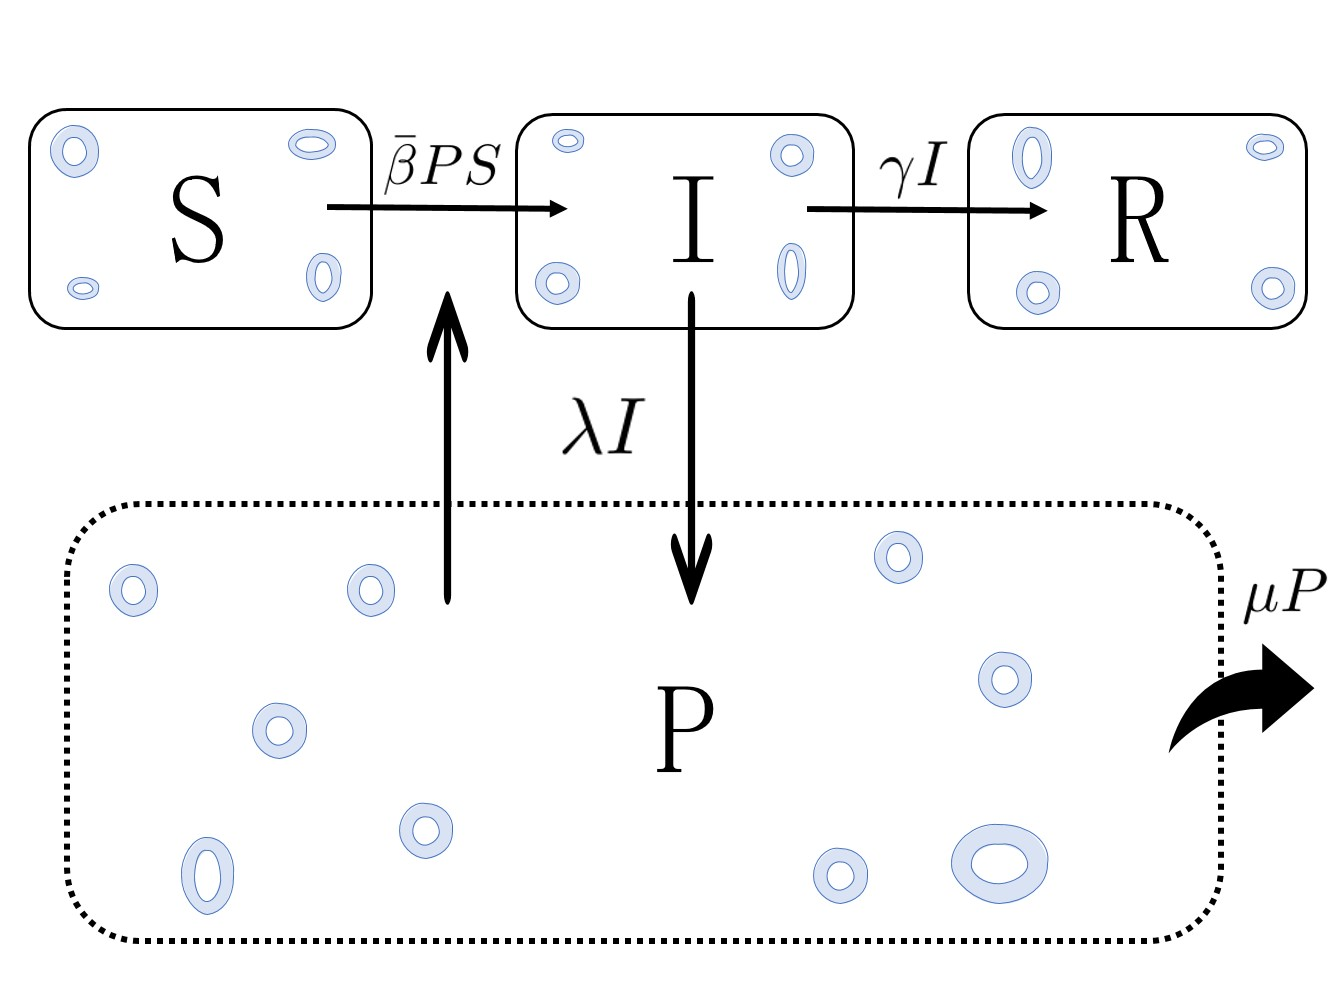
\includegraphics[width=1\textwidth]{Figures/SIRP_scheme_mod.jpg}
    \caption{SIRP model flow diagram. The model variables are represented
        by capital letters: susceptible hosts ($S$), infected hosts ($I$), dead
        hosts
        ($R$) and the population of parasite ($P$). Arrows represent the
        processes in
        the model with their rates indicated next to them and blue rings
        represent
        parasites. The flow follows the scheme in \cref{eq:scheme_reinfection},
        that
        leads to the system of differential equations in \cref{eq:SIRP}.}
    \label{fig: SIRP_scheme}
\end{figure}

\begin{table}[H]
    \centering
    \caption{Model parameters description}
    \begin{tabular}{cl:cl}
        \hline \hline
        Variable & Definition             & Parameter & Definition
        \\ \hline
        $S$      & Susceptible host       & $\beta$   & Disease transmission
        rate                                                                 \\
        $I$      & Infected host          & $\gamma$  & Host mortality rate
        \\
        $R$      & Removed host           & $\lambda$ & Production rate of
        parasites by
        infected hosts
        \\
        $P$      & Parasite in the medium & $\mu$     & Parasite
        deactivation/dilution rate
        \\ \hline \hline
    \end{tabular}
    \label{tab:parameters}
\end{table}

Following this argumentation, the scheme in \cref{eq:scheme_reinfection}
and \cref{fig: SIRP_scheme}, one can write the evolution equations of the SIRP
model,
\begin{equation}\label{eq:SIRP}
    \begin{aligned}
        \dot{S} & =-\bar{\beta} P S                    \\
        \dot{I} & =\bar{\beta} P S-\gamma I            \\
        \dot{R} & =\gamma I                            \\
        \dot{P} & =\lambda I-\bar{\beta} P S-\mu P \ .
    \end{aligned}
\end{equation}
Model (\cref{eq:SIRP})	\textit{lives} in the $4$-dimensional (S,I,R,P)
phase space, representing the variables
the populations of individuals in the susceptible, infected and removed
host compartments and of parasites, respectively. These variables could be
redefined so that S, I and R represent proportions of hosts in each compartment
and P the population of parasites per host.

The fixed points of \cref{eq:SIRP} are determined by the
conditions\footnote{We do not consider the trivial fixed point $S=I=R=P=0$ that
    would imply $N=0$ and $P=0$ at all time.}
$I=P=0$, to be fulfilled simultaneously.
We will study the stability of the fixed point defined by $S(0)$,
$I(0)=P(0)=0$ and $R(0)=N-S(0)$.
A linear stability analysis of this fixed point reveals that it has two
null eigenvalues, that stem from the condition $N=S+I+R$ and the conserved
quantity of \ref{app:P_exact}.
The first condition, $S+I+R=N$, implies that it is enough to consider two
of the host populations, e.g. $S$ and $I$, as the third one can be obtained
from the other two. The implications of the conserved quantity reported in
\ref{app:P_exact} are more subtle, as it implies that fixed points are not
isolated, as it happens in ordinary dissipative dynamical systems, and there is
an infinite number (a line of) fixed points for the final state of the
epidemic, depending on the initial conditions. This also implies that the phase
space is foliated by the conserved quantity, $C$ of
\cref{eq:conservedquantity}, and every initial condition, $S_0$, with a
different value of $C$ leads to a different asymptotic condition, $S_{\infty}$,
just as shown in \cite{Murray_book} for the SIR model (cf. Fig. 10.1 in
\textit{op. cit.}).
The third eigenvalue, that is the largest of the two non-zero eigenvalues,
can be positive if $\beta S_0 \lambda>\gamma(\beta S_0+\mu)$ and negative if
the inequality is reversed, defining the conditional stability of the fixed
point. The fourth eigenvalue is always negative and all the eigenvalues are
always real (cf. \ref{app:linstabfp}).
The instability of the fixed point along the third eigenvalue drives the
beginning of the epidemic.

An extremely important result in epidemiology is the so-called
\textit{basic reproduction number}, $R_0$, a dimensionless number which
represents the number of secondary infections produced by a primary infection
in a fully susceptible population. $R_0=1$ defines the threshold for epidemic
propagation: an epidemic will occur when $R_0>1$, and the number of infected
individuals will grow, at an exponential rate in the early phases of the
epidemic \cite{Castro2020}, while if $R_0<1$ the infection will wane
naturally.
This quantity can be formally obtained making use of the Next Generation
Matrix (NGM) method \cite{Theory_next_gen_matrix, Diekmann2010}. Applying this
formal method to our system of ordinary differential equations (ODE's) one
obtains the following relation for the basic reproduction number (cf.
\ref{app:NGM}),
\begin{equation}\label{eq:R_0_SIRP}
    R_0=\frac{\lambda}{\gamma\parentesi{1+\displaystyle\frac{\mu}{\bar{\beta}
                S(0)}}} \ .
\end{equation}

The threshold condition provided by $R_0$ (\cref{eq:R_0_SIRP}) is
equivalent
to the linear stability condition for the third eigenvalue of the initial,
pre-epidemic, fixed point, as $\bar{\beta} S(0) \lambda>\gamma(\beta S(0)+\mu)$
implies that this eigenvalue is positive and the disease-free equilibrium
state unstable being this
equivalent to $R_0>1$ (cf. \ref{app:linstabfp}).
Thus, if $R_0>1$ the fixed point is unstable, and an epidemic will ensure
if infected hosts, $I$, or parasites, $P$ appear in the system. An epidemic
will propagate until the system reaches an stable fixed point, that signals the
end of the epidemic (cf. \ref{app:linstabfp}).

\subsection{Model reduction} \label{sec:reduction}

The SIRP model lives in a $4$-dimensional phase space and depends on $4$
parameters, what makes difficult to confront it with experimental data. Thus,
we will discuss here
three alternative ways of reducing the model. The first involves an exact
reduction of the model, based on the conserved quantity derived in
\ref{app:P_exact}. The second reduction consists of an approximation to the
previous exact reduction, that turns out to be equivalent to an exact reduction
of a slightly simplified model (without the $-\bar{\beta}SP$ term in the
equation of $\dot{P}$). The third one is based on an approximation valid if the
system parameters fulfil certain conditions.

\subsubsection{Exact reduction of the SIRP model} \label{sec:exactred}

From the conserved quantity derived in	\ref{app:P_exact}, it is possible
to write the parasite population in the SIRP model as a function of the host
states as follows,
\begin{equation}\label{eq:P_exact}
    P(S,I)=-\frac{\lambda}{\gamma}\parentesi{S+I} +
    \frac{\mu}{\bar{\beta}}\ln(S) + S + C(0) \ ,
\end{equation}
where $C(0)=P(0)+\displaystyle\frac{\lambda}{\gamma}\parentesi{S(0)+I(0)} -
    \frac{\mu}{\bar{\beta}}\ln(S(0)) - S(0)$.\\

Substituting \cref{eq:P_exact} into the general SIRP model of
\cref{eq:SIRP} we obtain the following nonstandard SIR model,
\begin{equation}\label{eq:SIR_exact}
    \begin{aligned}
        \dot{S} & = \frac{\lambda\bar{\beta}}{\gamma}S\parentesi{S+I} - \mu
        S\ln(S) - \bar{\beta} S^2 - S\bar{\beta} C(0)                        \\
        \dot{I} & = -\frac{\lambda\bar{\beta}}{\gamma}S\parentesi{S+I} + \mu
        S\ln(S) + \bar{\beta} S^2 + S\bar{\beta} C(0) -\gamma I              \\
        \dot{R} & =\gamma I \ .
    \end{aligned}
\end{equation}

Although using the conserved quantity yields an exact reduction from a 4D
dynamical system to a 3D one, the number of independent parameters and initial
conditions remain unchanged, i.e. they still depend on $4$ parameters and $4$
initial conditions. Thus, although useful, (\ref{eq:SIR_exact}) is not ideal
when trying to fit experimental data, and this is the reason for trying a
further approximation to \cref{eq:SIR_exact} to be discussed next.

\subsubsection{Further approximation to the exact reduction}
\label{sec:exactredapp}

A further approximation to \cref{sec:exactred}, that is less restrictive
and expected to be valid in a broader parameter range than \cref{sec:fastslow}
is possible. This approximation reduces the number of free parameters by one,
what is useful in fitting available data.
The approximation consists of neglecting the
$S$ term in \cref{eq:P_exact}, what is possible if $\lambda/\gamma\gg 1$
and also $\mu\ln N/(\bar{\beta} N)\gg 1$, as $S(t)$ decreases monotonically
with time and is, at most, $N$ at the initial time. Interestingly, this
approximation is equivalent to the simplification of the equation for $\dot{P}$
in (\ref{eq:SIRP}) so that the $-\bar{\beta}SP$ is skipped, what yields exactly
the SIP model of Ref. \cite{article_SIP}. This reduced model has an exact
conserved quantity, $\mathcal{C}$, that differs from that of the SIRP model in
the linear $S$ term (cf. \ref{app:P_exact}).
Using this approximation one can write,
\begin{equation}\label{eq:SIR_exact_reduced}
    \begin{aligned}
        \dot{S} & =\frac{\lambda'}{\gamma}S(S+I)-\mu
        S\ln(S)-S\bar{\mathcal{C}}(0)                 \\
        \dot{I} & =-\frac{\lambda'}{\gamma}S(S+I)+\mu
        S\ln(S)+S\bar{\mathcal{C}}(0)-\gamma I        \\
        \dot{R} & =\gamma I \ ,
    \end{aligned}
\end{equation}
where $\lambda'=\lambda\bar{\beta}$ and $\bar{\mathcal{C}}(0)=\bar{\beta}
    (P(0)+\lambda/\gamma(S(0)+I(0)-\mu/\bar{\beta}\ln S(0)))=\bar{\beta}
    \mathcal{C}(0)$ is a redefinition of the conserved quantity of the SIP
model
\cref{eq:conservedquantitySIP}, $\mathcal{C}(0)$, a constant, such that it
absorbs $\bar{\beta}$ and all initial conditions of the model. The result is
that \cref{eq:SIR_exact_reduced} depends on $3$ parameters and $1$ constant,
compared to \cref{eq:SIR_exact} that depends on $4$ parameters,
facilitating, thus, the use of the model to fit experimental data.

\subsubsection{Model reduction through fast-slow separation}
\label{sec:fastslow}

The third
reduction of the $4$-D dynamical model \cref{eq:SIRP} makes the assumption
that
the time scale in which the parasite population changes are faster than the
one corresponding to the host. This means that pathogen deactivation in the
medium must be faster than host mortality. In terms of the rates associated to
each of these processes, this means $\mu>\gamma$. Taking $\mu$ as common factor
in $\dot{P}$ one can write,
\begin{equation}
    \epsilon \dot{P} =\lambda I/\mu-\bar{\beta}SP/\mu-P
\end{equation}
where $\epsilon=1/\mu$ is small, as $\mu$ is large. If furthermore
$\mu\gg\bar{\beta}N$ and  $\lambda\gg \beta P$ one arrives to,
\begin{equation}\label{eq:P_approx}
    P\approx \frac{\lambda}{\mu} I \ .
\end{equation}

Under this approximation the slow subsystem can be written,
\begin{equation}\label{eq:SIRslow}
    \begin{aligned}
        \dot{S} & =-\beta' I S         \\
        \dot{I} & =(\beta' S-\gamma) I \\
        \dot{R} & =\gamma I\ ,
    \end{aligned}
\end{equation}
that is equivalent to the classical SIR model with $\beta'=\bar{\beta}
    \lambda/\mu$ instead of the infection rate $\bar{\beta}$. The reduced $3$-D
model \cref{eq:SIRslow} from the original $4$-D SIRP model \cref{eq:SIRP}
depends on $2$ parameters instead of $4$ as the original model had and $1$
initial condition, e.g. $I(0)=N-S(0)$ if $R(0)=0$, and is much more amenable to
be applied to the analysis of experimental data, as shown in
\cref{sec:validation}.
Furthermore, $\gamma$ could be eliminated through a time rescaling,
$t\rightarrow=t'=\gamma t$ with a redefinition of
$\beta'\rightarrow\beta''=\beta'/\gamma=\beta\lambda/(\mu\gamma)$, leaving the
model as a function of a single effective parameter. However, we will keep both
$\beta'$ and $\gamma$ for convenience when fitting the model to experimental
data in \cref{sec:validation}, as we would need to know anyhow $\gamma$ in
order to analyse the experimental data. The validity of this approximation is
checked numerically in \cref{sec:numericalanalysis}.

\section{Numerical analysis of the model} \label{sec:numericalanalysis}

Due to the impossibility of solving the SIRP model analytically,
in the present section we perform a numerical characterisation of the
model\footnote{All numerical simulations of the dynamical system
    \cref{eq:SIRP} have been carried out using a Runge-Kutta $4$th order
    method,
    with a temporal step $\Delta t=0.001$. Numerically stable results are
    obtain
    with $\Delta t\le 0.01$.}.
Moreover, we show the validity range of the performed approximations to
reduce the SIRP model to an effective SIR model. We start our numerical
analysis by investigating the relative influence of the model parameters on
some epidemiological quantities of interest: the basic reproduction number
($R_0$), related to the existence of an epidemic outbreak, continuing with the
final state of the epidemic, given by the final number of dead individuals
($R(\infty)$) and the maximum of infected individuals ($I_{\textrm{max}}$)
together with the time at which it occurs ($t_{\textrm{max}}$).

In order to identify the most influential parameters of our model
Sensitivity Analysis (SA) will be performed. SA can be divided into two
classes: Local Sensitivity Analysis (LSA) and Global Sensitivity Analysis
(GSA). LSA represents the assessment of the local impact of input factors
variation on model response by concentrating on the sensitivity in the vicinity
of a set of factor values. Such sensitivity is often evaluated through
gradients or partial derivatives of the output functions at these factor
values, such that other input factors are kept constant.
Since epidemic models exhibit a threshold behaviour, controlled by the
dimensionless quantity
$R_0$, it is relevant to study its robustness with respect to small
perturbations by means of the LSA explained above, as its analytical expression
is known.

On the other hand, GSA will be applied to study the influence of the
parameters in the final state of the epidemic and the epidemic peak by
exploring a large domain of the parameter space. In turn, GSA is the process of
apportioning the uncertainty in outputs to the uncertainty in each input factor
over their entire range of interest. A sensitivity analysis is considered to be
global when all the input factors are varied simultaneously and the sensitivity
is evaluated over the entire range of each input factor, in clear contrast to
LSA. Within GSA, first order indices are a measure of the contribution to the
output variance given by the variation of the parameter alone averaged over
variations in other input parameters while second order indices take into
account first order interactions between parameters. While LSA is carried out
analytically (if exact expressions are available), GSA is a purely numerical
approach. Further mathematical details on Sensitivity Analysis can be found in
\ref{app:sensanal}.

For all the sensitivity analysis performed in the following sections, and
in order to avoid ambiguities associated to the definition of $\bar{\beta}$ as
a function of $N$, we assume $N=1$, so that both possible incidences yield
$\bar{\beta}=\beta$ and the numerical results are equivalent.

\subsection{The basic reproduction number $R_0$}

To study the relevance of parameters involved in an epidemic outbreak a LSA
was performed. We analyse the local sensitivity of $R_0$ through the normalised
sensitivity index, so that the function $F(\vec{p})$ of
\cref{eq:sensitivity_analysis} is substituted by the analytical expression of
$R_0$, \cref{eq:R_0_SIRP}.

\cref{fig:Local_Sensitivity_Analysis_R0}(a) shows the sensitivity index for
$R_0$ for specific baseline parameters, where $\lambda$, $\bar{\beta}$ and
$S_0$ contribute to increase the basic reproduction number while $\alpha$,
$\gamma$ and $\mu$ contribute to decrease it, as expected. Moreover, we can see
that $\lambda$ and $\gamma$ are the most influential parameters while $\mu$,
$\bar{\beta}$ and $S_0$ depend on each other. These dependencies cause varying
influences on $R_0$, which are fully depicted in panels
\cref{fig:Local_Sensitivity_Analysis_R0}(b-d). It can be seen that the
influence of $\bar{\beta}$ increases with the increase of $\mu$ and the
decrease of $S_0$. Similarly, the importance of $S_0$ increases with $\mu$ and
decreases with $\bar{\beta}$. On the other hand, the impact of $\mu$ increases
with the decrease of both $S_0$ or $\bar{\beta}$.

\begin{figure}[H]
    \centering
    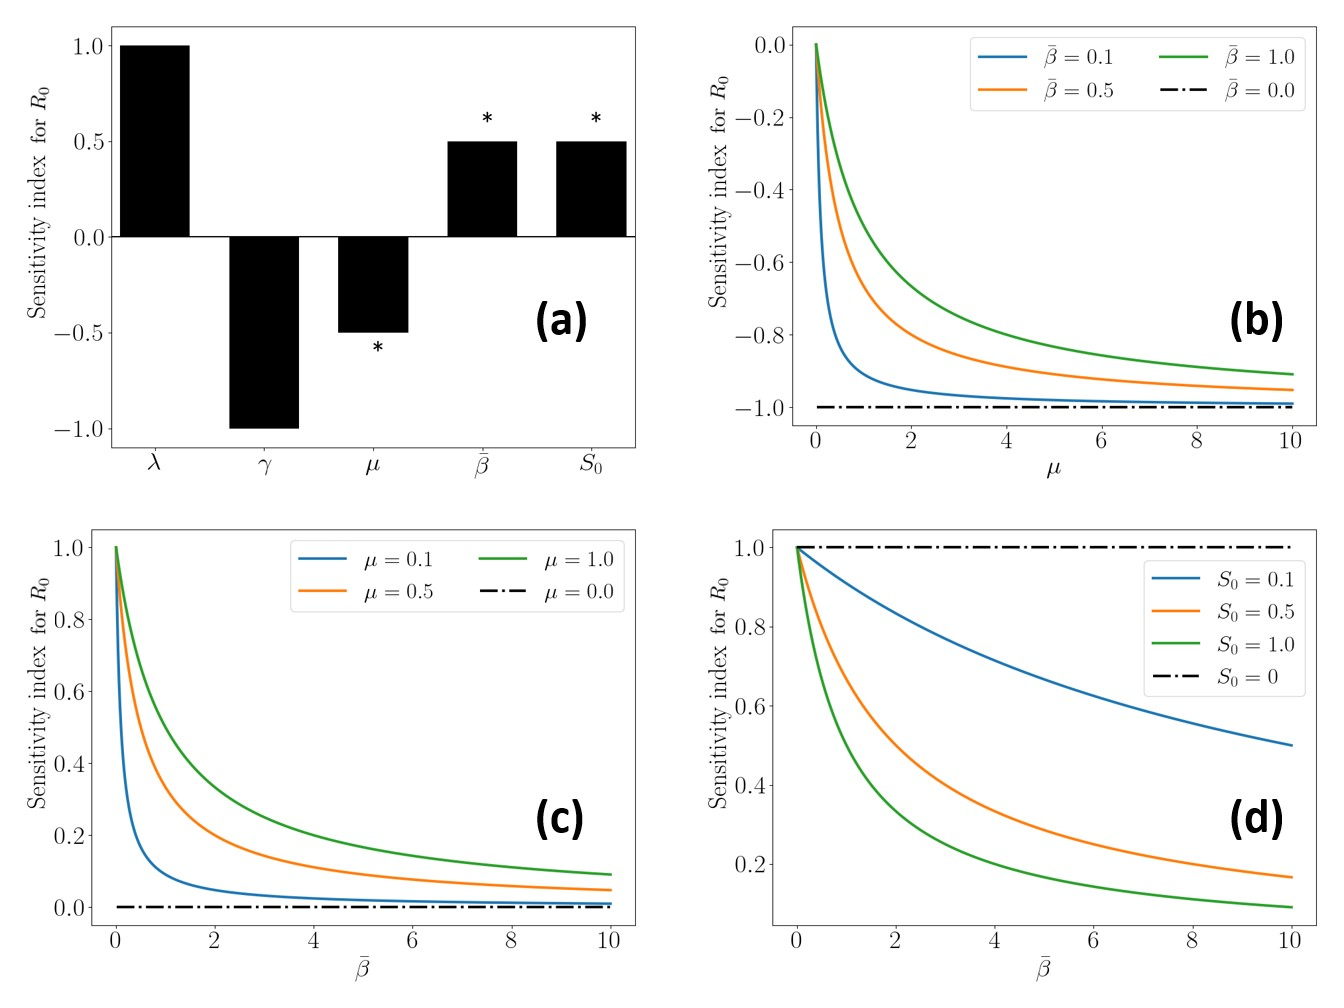
\includegraphics[width=1\textwidth]{Figures/R_0_sensitivity.jpg}
    \caption{Panel (a): Local sensitivity analysis of $R_0$ for the
        baseline parameters $\lambda=1$, $\gamma=1$ and
        $\mu=\bar{\beta}=S_0=1$. The
        asterisks mark parameters for which the sensitivity index is not
        constant,
        depending on, at least, another parameter. Panels (b-d): Local
        sensitivity
        analysis of $R_0$ with respect to parameters with an asterisk, showing
        the
        different dependence with a second parameter and the effect on the
        varying
        sensitivity index.}
    \label{fig:Local_Sensitivity_Analysis_R0}
\end{figure}

\subsection{Final state of the epidemic}

Another important quantity in epidemiology is the final state of the
epidemic, which can be characterised by the final number of dead individuals,
$R_\infty$. Within our general SIRP model it is not possible to find an
analytical expression of $R(t)$ so that we need to tackle the problem
numerically. To this end, we perform GSA for the final number of dead
individuals in order to determine the most influential parameters for this
quantity. In particular, we apply the Sobol method, discussed in
\ref{app:sensanal}.
The Confidence Interval, CI, obtained in our
study is less than 1\% of the index value, indicating a very high accuracy,
therefore it is not shown in the figures. The results of the explained
procedure are shown in \cref{fig: GSA_R_inf}, where the total order (black),
first order (white) and second order (gray) sensitivity indices for each of the
model parameters are detailed. It can be observed that $\mu$ has a slightly
greater influence than the other parameters with respect to the final number of
dead individuals. Note that the second order indices are larger than the first
order ones for all the parameters, which indicates a high influence of the
nonlinearities in our model, at least for the particular quantity under study.

\begin{figure}[H]
    \centering
    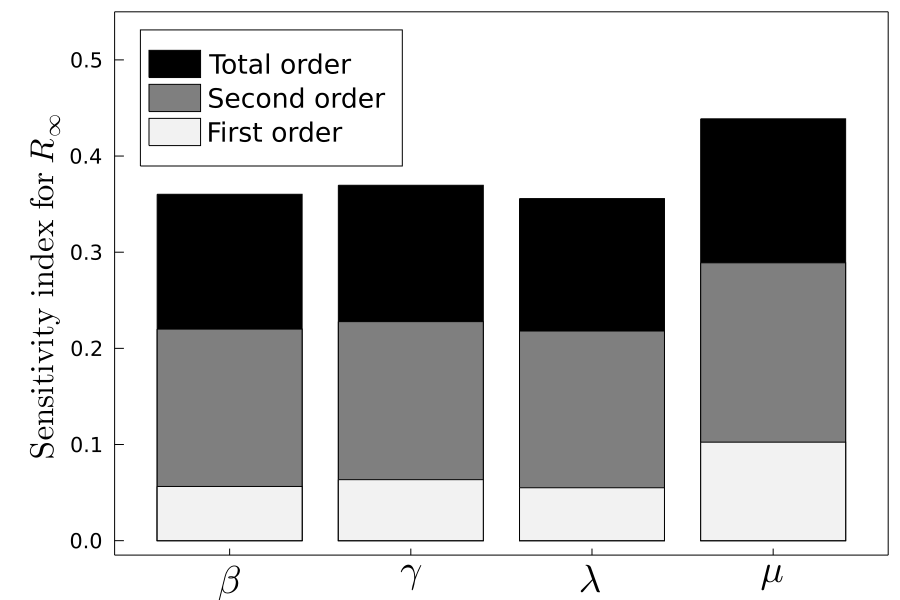
\includegraphics[width=0.7\textwidth]{Figures/GSA_R_inf.png}
    \caption{Sensitivity indices (LSA) for the final number of dead
        individuals ($R_\infty$) for each one of the indicated parameters. The
        black
        bars represent the total order indices of sensitivity while white
        (grey) colour
        represents the contribution of the first (second) order indices.}
    \label{fig: GSA_R_inf}
\end{figure}

\begin{figure}[H]
    \centering
    \subfigure[Epidemic
        peak]{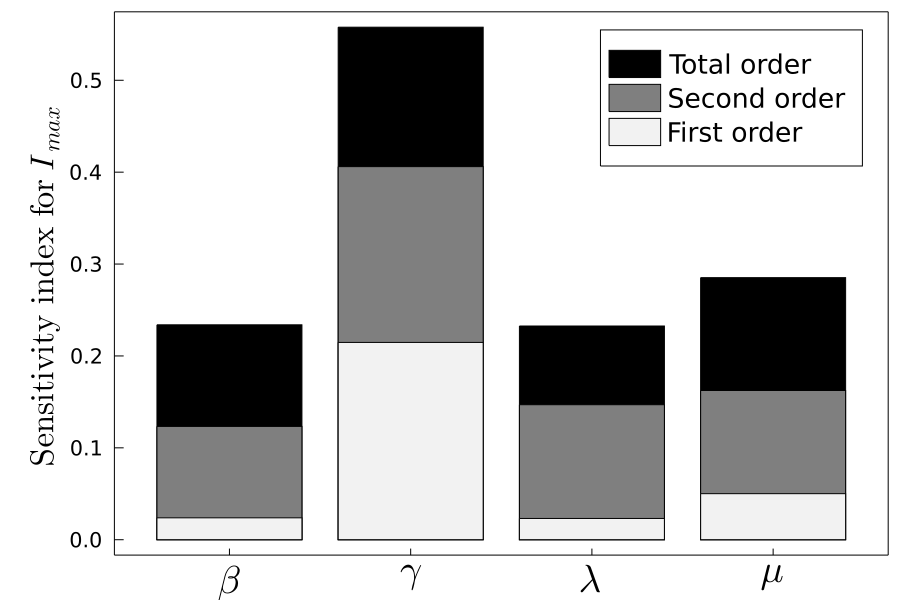
\includegraphics[width=0.49\textwidth]{Figures/GS_peak.png}}
    \subfigure[Time of epidemic
        peak]{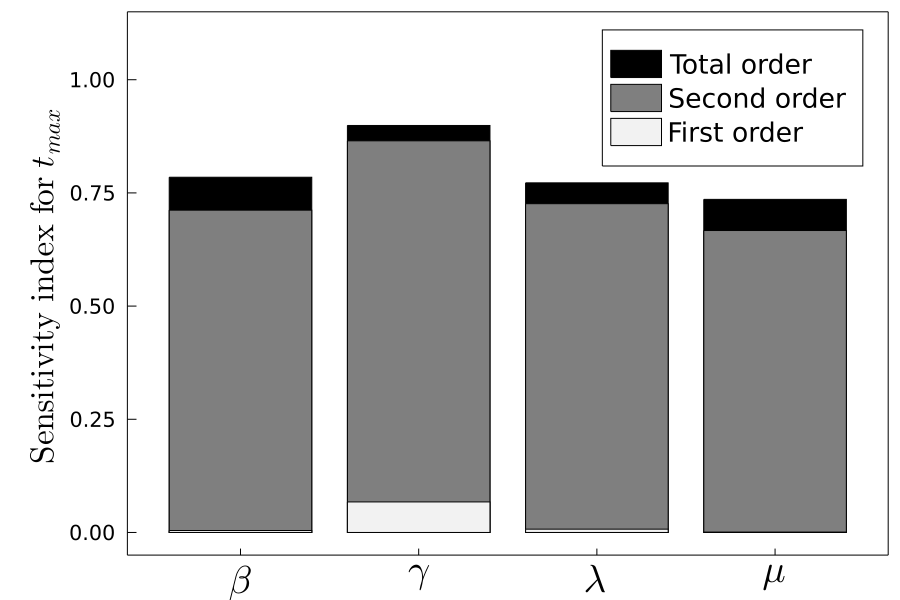
\includegraphics[width=0.49\textwidth]{Figures/GS_peak_time.png}}
    \caption{Global sensitivity analysis for the maximum of infected
        individuals $I_{\textrm{max}}$ (a) and its time occurrence
        $t_{\textrm{max}}$
        (b). The black bars represent sensitivity at all orders,
        while white (grey) colour represents the contribution of the first
        (second) order indices.}
    \label{fig: GS_analysis}
\end{figure}

\subsection{Maximum of infected individuals}

A GSA of the maximum number of infected individuals, $I_{\textrm{max}}$ and
the time it occurs, $t_{\textrm{max}}$ is performed to study the influence of
the model parameters regarding these quantities. In this case, \cref{fig:
    GS_analysis}, $\gamma$ has greater influence in the epidemic peak than any
of
the other parameters, while for the time at which the peak takes place, all the
parameters have basically the same influence. Again, the second order indices
(the first order interactions between parameters) account for most of parameter
sensitivity, in particular in the time of the epidemic peak, indicating the
high degree of nonlinearity of this effect.

\begin{figure}[H]
    \centering
    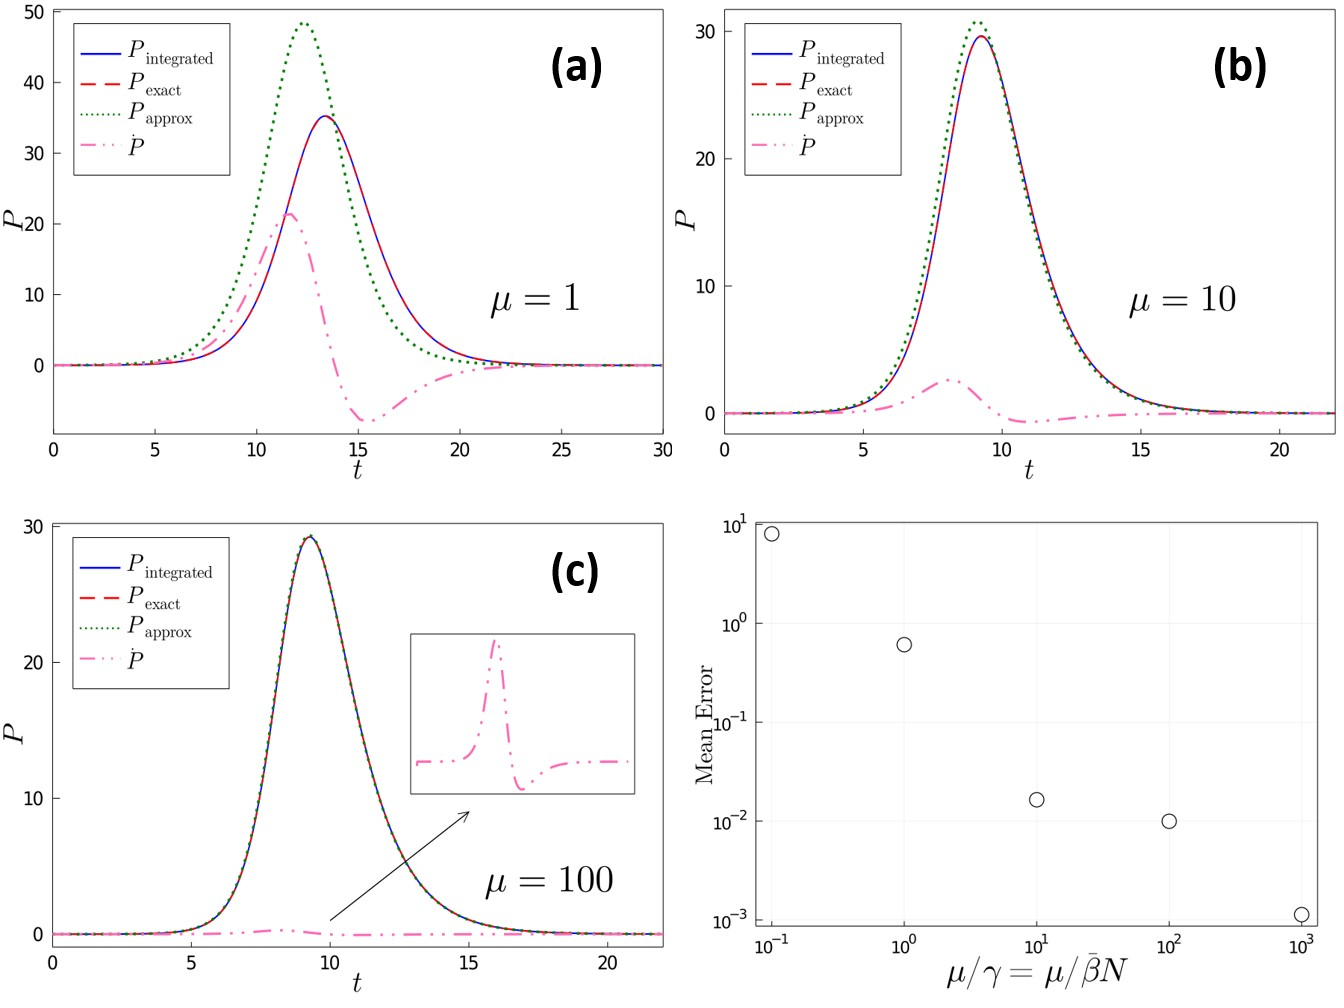
\includegraphics[width=1\textwidth]{Figures/P_comparison.jpg}
    \caption{Numerical check of the approximate expression for the pathogen
        concentration, (\cref{eq:P_approx}), $\bar{\beta}=1/50$ and $\gamma=1$:
        (a)
        $\mu=1$; (b) $\mu=10$; (c) $\mu=100$, while $\lambda$ is varied to keep
        $R_0=2.5$, defined in (\cref{eq:R_0_SIRP}) (with $S_0=N=50$), i.e.,
        $\lambda=5,
            27.5, 252.5$ respectively for (a)-(b)-(c), respectively.
        The blue solid line represents the numerically integrated quantity, the
        red dashed line (superimposed to the blue solid one as they are
        identical) is
        the exact solution for this quantity, (\cref{eq:P_exact}) and the green
        dotted
        line accounts for the approximate expression from the timescale
        separation
        (\cref{eq:P_approx}). The dash-dotted pink line represents the
        derivative of
        $P$, $\dot{P}$, in the scaled time frame. Panel (d): Mean error between
        the
        approximate and exact solutions for increasing
        $\mu/\gamma=\mu/\bar{\beta}$.}
    \label{fig:P_comparison}
\end{figure}

\subsection{Numerical verification of the fast-slow approximation}

The parasite concentration approximation, based on a timescale separation
discussed in \cref{sec:fastslow}, is now verified by computational means. The
verification was performed using both mass action and standard incidence, but
for the sake of simplicity we show only the results for the standard incidence
case. Worth is to say that, mathematically, changing from standard incidence to
mass action involves only a rescaling of the $\beta$ parameter, so that the
numerical results are exactly the same. \cref{fig:P_comparison} contains a
comparison for $3$ different values of the parasite deactivation rate, $\mu$.
It can be seen that the approximation is poor when $\mu\sim
    \gamma,\bar{\beta}N$ \cref{fig:P_comparison}(a), as it could be expected.
On
the other hand, the approximation is quite good when $\mu$ is one order of
magnitude larger than $\gamma$ and $\bar{\beta}N$ \cref{fig:P_comparison}(b),
while it is extremely accurate when $\mu$ is two orders of magnitude larger
than $\gamma,\bar{\beta}N$, \cref{fig:P_comparison}(c). The figure also shows
the numerical value of $\dot{P}$ (pink dashdot), and it can be checked how it
becomes smaller as $\mu$ increases compared to $\gamma,\bar{\beta}N$,
justifying the timescale separation of \cref{sec:fastslow}. Finally,
\cref{fig:P_comparison}(a-c) also shows (dashed red line) the analytical value
for $P(S,I)$ derived in \cref{eq:PSI_exact}, that matches perfectly the result
of the numerical integration of \cref{eq:SIRP}, as should be the case.

\begin{figure}[H]
    \centering
    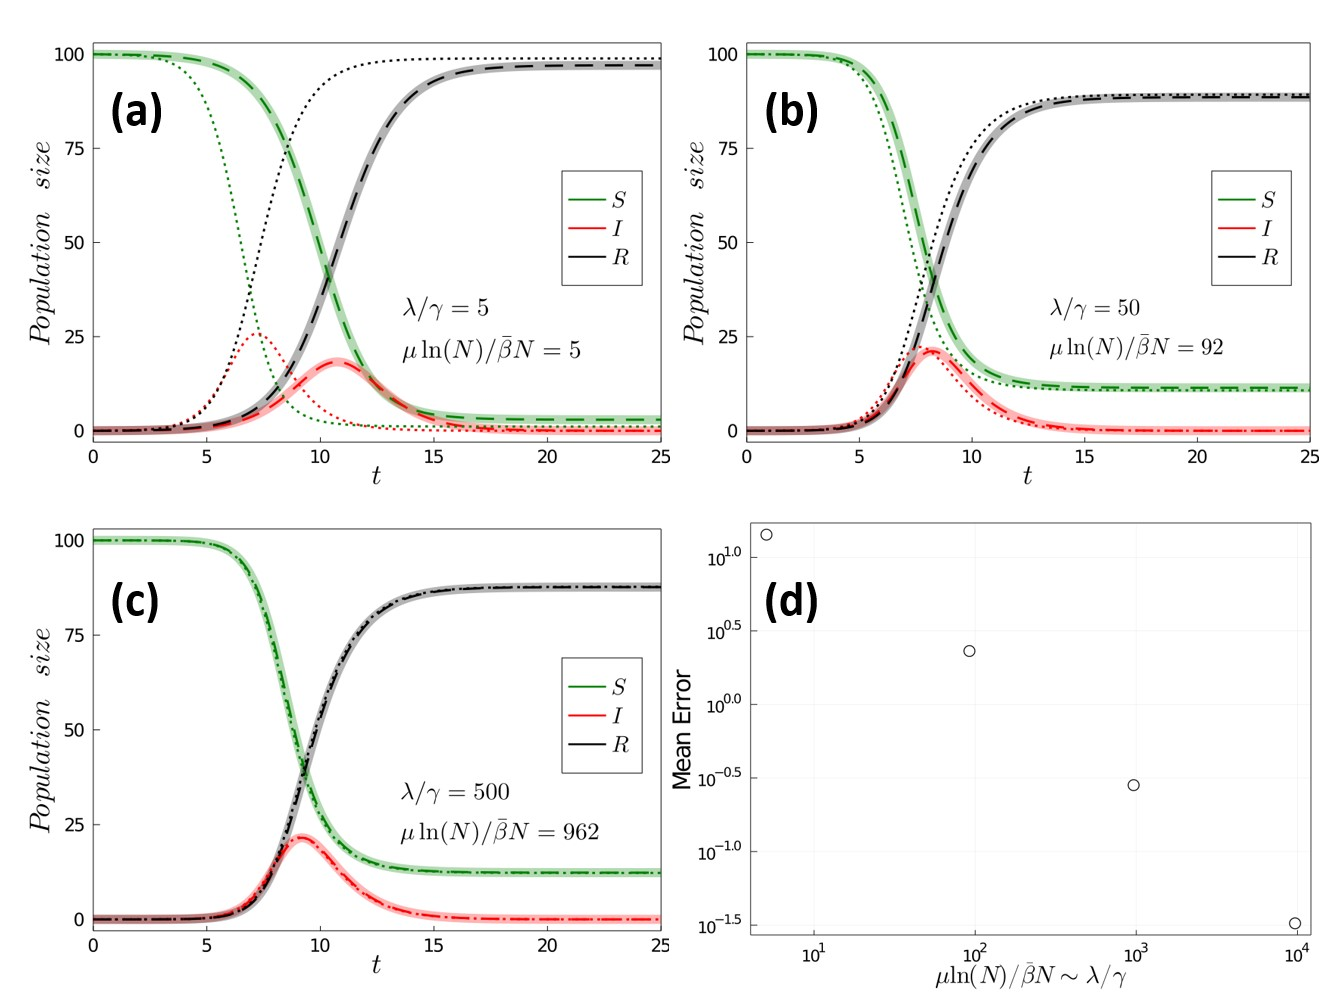
\includegraphics[width=1\textwidth]{Figures/exact_reduction_approx.jpg}
    \caption{Numerical check of the exact model reduction along with the
        subsequent approximation shown in \cref{sec:exactred} with $N=100$,
        $\bar{\beta}=1/100$, $\gamma=1$, (a) $\lambda=5$, $\mu=1.1$; (b)
        $\lambda=50$,
        $\mu=20$; (c) $\lambda=500$, $\mu=209$. $R_0=2.38$ for all the panels.
        The
        solid semitransparent lines represent the original 4D model, the dashed
        lines
        the exact reduction and the dotted lines the approximate model from the
        exact
        reduction. Panel (d): Mean error between the approximate and exact
        solutions
        for increasing $\mu\ln(N)/\bar{\beta}N$ and $\lambda/\gamma$ while
        $R_0=2.38$
        is kept constant.}
    \label{fig:verification_exact_reduction}
\end{figure}

\subsection{Numerical verification of the model approximation from the
    exact reduction} \label{sec:apprexred}

The numerical verification was performed for both mass action and standard
incidence, but for the sake of simplicity in
\cref{fig:verification_exact_reduction} we show only the results for the
standard incidence case. First, and as it should be because it is an exact
result, the exact reduction of the SIRP model discussed in \cref{sec:exactred}
matches perfectly the numerical results obtained from the full model for all
possible parameter values,
\cref{fig:verification_exact_reduction}(a-c).
Regarding the approximation to the exact reduction, one can see
how the approximation converges to the exact solution as the parameters
fulfil the conditions indicated in \cref{sec:exactredapp}, namely that both
$\gamma/\lambda\gg 1$ and $\mu\log(N)/\bar{\beta N}\gg 1$, becoming very
accurate if these ratios are larger than $1$ by two orders of magnitude or more
(cf.  \cref{fig:verification_exact_reduction}(c)). We recall that in this case
the SIRP model converges to the SIP model of \cite{article_SIP}. Conversely,
the approximation is poor when any of these two ratios is of order $1$ ((cf.
\cref{fig:verification_exact_reduction}(a))), while
\cref{fig:verification_exact_reduction}(b) presents the result in an
intermediate case, in which the approximation is fair.

\section{Model validation with data of the \textit{Pinna nobilis} Mass
  Mortality Event}
\label{sec:validation}

In this section, the general SIRP model is validated against collected data
from the \textit{Pinna nobilis} Mass Mortality Event. As explained in
\cref{sec:Introduction_Nacras_I}, the disease is caused by the parasite
\textit{Haplosporidium pinnae} and the hosts, \textit{P. nobilis}, are sessile
bivalves endemic of the Mediterranean Sea. Thus, this epidemic is a perfect
candidate to be described by the SIRP model. In the model, parasite production
occurs only inside infected hosts, and parasites are released to the medium,
either through their respiratory or digestive system. The simultaneous
occurrence of the different possible stages of the parasite (uni- and
bi-nucleate cells, multinucleate plasmodia, sporocysts and uninucleate spores)
in the same host individual is not common among haplosporidans and makes
\textit{H. pinnae}  different from previously known haplosporidan species
\cite{CATANESE20189}. The occurrence of uni- and binucleate stages suggest
possible direct transmission from infected to healthy fan mussels, as observed
in \textit{B. ostreae} and \textit{B. exitiosa} \cite{hine1996ecology,
    Culloty2007, Audemard2014}. Additionally, the presence of spores (a
dormant,
resistant stage) could allow long persistence in the environment and the
hypothetical involvement of an intermediate host as suggested for \textit{H.
    nelsoni} and \textit{H. costale} \cite{Andrews1984,
    haskin1988uncertainties,
    powell1999modeling}. While uninucleate cells are always detected in
infected
fan mussels, sporulation has been only detected sporadically
\cite{CATANESE20189}. Thus, we assume that infection occurs mostly through
uninucleate (or binucleate) cells by direct transmission (as the experimental
observations in captivity point out, see \cite{March}).
We do not consider disease transmission through other stages. We do not
consider spores, given the infrequent observation of spores and the current
lack of experimental information about spore transmission (that could involve
another intermediate host species). Regarding plasmodia and sporocyst stages,
these stages are too large to be released through the epithelium. The
distinction between uninucleate and binucleate cells seems unnecessary at this
level of representation, as these phases only participate in parasite
proliferation inside infected hosts, a process that we consider in an effective
way. Finally, the evidence of the time course of the disease compared to the
long life cycle of {\it P. nobilis\/} suggests host vital dynamics (i.e.
recruitment (reproduction) and natural death) can be neglected.

After an epidemic outbreak that took place in Portlligat, in the north east
of Catalonia, $215$ \textit{Pinna nobilis} individuals were extracted from
their natural medium in order to be preserved as a genetic reserve in several
controlled water tanks of different institutions in Spain \cite{March}. The
institutions that participated in this preservation effort were IFAPA, IEO,
IRTA, IMEDMAR-UCV and Oceanogr\`afic of Valencia. The original idea was to
rescue the individuals before infection, however, the subsequent evolution of
the rescued \textit{Pinna nobilis} populations indicates that some individuals
were already infected at the time of extraction (and/or in contact with some
amount of the parasite transferred from sea water).
This allowed the opportunity to use the data of the time evolution of the
epidemic in the controlled water tanks, reported in \cite{March}, to evaluate
the described SIRP model\footnote{Data use in this work with the purpose of
    validating and fitting parameters for the SIRP model have been taken from
    the
    Supplementary Information of \cite{March}}. The empirical data consists of
the
proportion of survivors as a function of time in the controlled water tanks
with a temporal resolution of one month. Despite the fact that the temperature
of the water in the tanks was controlled, it was sharply lowered in most of the
tanks when mortality started to appear within the population, as a last effort
to keep the rest of the population safe and alive, since keeping the
temperature below  approximately $13.5\, {}^o$C is a known strategy to preserve
\textit{Pinna nobilis} individuals as disease expression is minimal
\cite{Cabanellas2019}. Fortunately, two of the tanks kept its temperature
approximately constant during the full recorded time. This is the case of the
tanks in IFAPA in Huelva and the Oceanogr\`afic of Valencia (OCE), both Spanish
institutes. These water tanks have been selected to validate our model,
maintaining constant temperatures of $14\, {}^o$C and $17\, {}^o$C,
respectively.

First we will fit the exact reduction of the SIRP model, assuming
$\mu\log(N)\gg\bar{\beta}N$ and $\lambda/\gamma\gg 1$ as discussed in
\cref{sec:exactredapp}, namely \cref{eq:SIR_exact_reduced}.
This reduced model depends on three parameters ($\lambda'$, $\mu$,
$\gamma$) and one constant, $\bar{\mathcal{C}}(0)$, cf. \cref{sec:exactredapp},
that is related to the initial conditions of the model. The order of magnitude
of the mortality rate can be deduced from data, with an estimate value of
$\gamma\approx\SI{1}{month^{-1}}$. We fix this parameter in order to give some
biological information to our model prior to the computational fit. We focus on
the $R$ compartment, as it can be retrieved directly from data in
\cite{March}\footnote{The number of dead individuals can be obtained as
    $R=N-S$, where $S$ is the population of survivors and $N$ is the total
    number
    of individuals in the tanks,
    $50$ (IFAPA) and $5$ (Oceanogr\`afic), respectively}.
We use a box-constrained variant\footnote{We constrain the optimisation
    because the unconstrained optimisation to the full range of the parameters,
    i.e, from $0$ to $\infty$ is not practical.} of the well known BFGS
optimisation algorithm \cite{BFGS} with a common $\textrm{L}2$ loss function,
also known as Residual Sum of Squares (RSS)\footnote{The algorithm is
    implemented within the Julia high-level programming language \cite{julia}
    using the DifferentialEquations.jl package
    \cite{DifferentialEquations.jl}.}.
By running this algorithm one observes that the optimal parameters tend to be
the ones in the boundary of the box-constrained parameter space.
Furthermore, if the box size is increased (or decreased) the optimal
parameters continue to be in the boundary of the box-constrained parameter
space.
This indicates that there exist several parameter combinations that
optimally fit the data, and the combination parameters found by the
optimisation algorithm are only marginally optimal with respect to other
parameter values. The locus (actually a valley) of marginal optimal parameters
can be seen in the right hand side panels of \cref{fig: exact_SIR_fit}, where
the cost function value of the optimisation algorithm is plotted as heat map.

\begin{figure}[H]
    \centering
    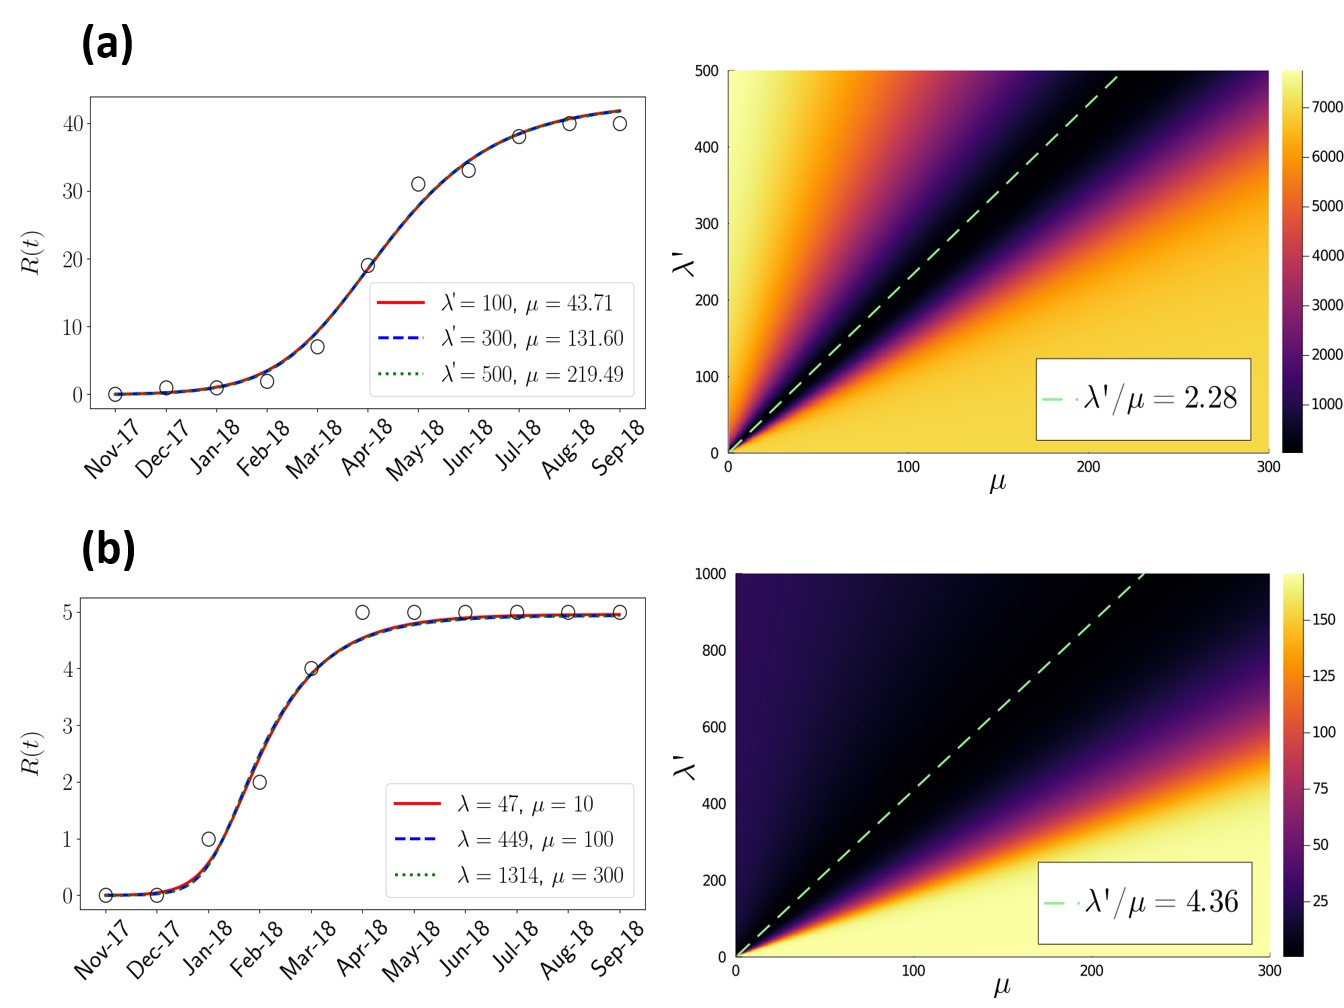
\includegraphics[width=1\textwidth]{Figures/exact_SIR_fitting.jpg}
    \caption{Parameter estimation for the approximation from the exact
        reduction of the SIRP model (\cref{eq:SIR_exact_reduced}) using data
        from IFAPA
        (panel (a)) and OCE (panel (b)) water tanks, at $\SI{14}{\degree C}$
        and
        $\SI{17}{\degree C}$ respectively. Left figures represent several fits
        of the
        model to empirical data of the number of dead hosts ($R(t)$) using
        different
        optimal combinations of the parameters. Right figures are the RSS
        errors as a
        function of the input parameters, where the green dashed line
        represents the
        set of optimal combinations of the parameters with $RSS=60, 0.8$ for
        IFAPA and
        OCE, respectively.}
    \label{fig: exact_SIR_fit}
\end{figure}

Now we reach the point regarding the dilemma between mass action and
standard incidence discussed in \cref{subsec:modtruct}. If one does not correct
the $\bar{\beta}$ parameter with the size of the host population, $N$, that is
equivalent to assuming the mass action incidence $\bar{\beta}=\beta$, the
values that one would obtain for $\beta'=\beta\lambda/\mu=\lambda'/\mu$ for
both populations take disparate values in both tanks: $\beta'=0.046$ for the
IFAPA data set and $\beta'=0.87$ for the Oceanogràfic (OCE) data set, a factor
of $19$ between them while their temperatures differ only by $3\,{}^o$C.
These numbers indicate that the standard incidence is more reasonable, what
amounts to choosing $\bar{\beta}=\beta/N$, where the final values of the
reported parameter $\beta'$ should be multiplied by $N=50$ for the IFAPA tank
and $N=5$ for the OCE tank. The final result is then $\beta'=2.28$ and
$\beta'=4.36$ for IFAPA and OCE tanks, that are the values reported in
\cref{fig: exact_SIR_fit}, implying that an almost twofold increase of the
$\beta'$ parameter corresponds to an increase of $3\,{}^o$C. This relation is
in good agreement with the typical changes in rates of a wide range of
organisms with a $\SI{3}{\degree C}$ change in temperature, while a 19-fold
change in the rate would imply at least a $\SI{30}{\degree C}$ change in
temperature (cf. \ref{app:rate_change}).

The fact that there is an infinite number of combinations of the parameters
that optimally fit the real data suggests that, as two parameters are slaved
one to each other, that the model
admits a further reduction. This reduction corresponds exactly to the
approximate $SIR$ model derived in \cref{eq:SIRslow}, with the relationship
$\beta'=\lambda'/\mu$, as anticipated. So, this gives further corroboration to
the use of the $SIR$ model \cref{eq:SIRslow} to fit $\beta'$ as the free
parameter (fixing the value of $\gamma$ and with $I_0$ as the initial condition
determined by the fit). For consistency with the previous fitting we expect to
obtain $\beta'=2.28$ and $4.36$ as the optimal parameters for the IFAPA and OCE
water tanks, respectively, and this is the case.

Interestingly, as reduced model \cref{eq:SIRslow} has fewer parameters to
fit we can relax our initial assumption of $\gamma=\SI{1}{month^{-1}}$ and
check how the fit improves or worsens when varying $\gamma$.
In \cref{fig:approx_SIR_fit} a fit of the reduced SIR model
\cref{eq:SIRslow} is shown for the IFAPA (top) and Oceanogràfic (bottom)
controlled water tanks\footnote{The $N$ correction corresponding to standard
    incidence has already been applied to these values.}.
\cref{fig:approx_SIR_fit}(c-d) shows the $RSS$ error as $\gamma$ is varied.
It can be seen that for the IFAPA water tanks $\gamma=\SI{1.5}{month^{-1}}$
yields more accurate results, while for the Oceanogràfic water tanks
$\gamma=\SI{1}{month^{-1}}$ remains optimum. This shows a decrease in the mean
removal time $1/\gamma$ for lower water temperatures, with the finite size
errors inherent to the OCE tank (as $N=5$).
In the left panels the simulated curve of dead individuals, $R$
compartment, as a function of time for the optimal fitted parameters is
confronted to the experimental data, showing a remarkable agreement. With the
optimum values of $\gamma$, in the IFAPA tank (now with
$\gamma=\SI{1.5}{month^{-1}}$) a new value of $\beta'=3.05$ is obtained,
implying a probably more reasonable ratio of $1.43$ for $\beta'$ in both tanks
(it was $1.91$ in the original fit).
From the optimal parameters we obtain the basic reproduction number, since
$R_0=\beta'/\gamma$ we have that $R_0^{\textrm{IFAPA}}\simeq2$ and
$R_0^{\textrm{OCE}}\simeq4$, clearly above the epidemic threshold.

\begin{figure}[H]
    \centering
    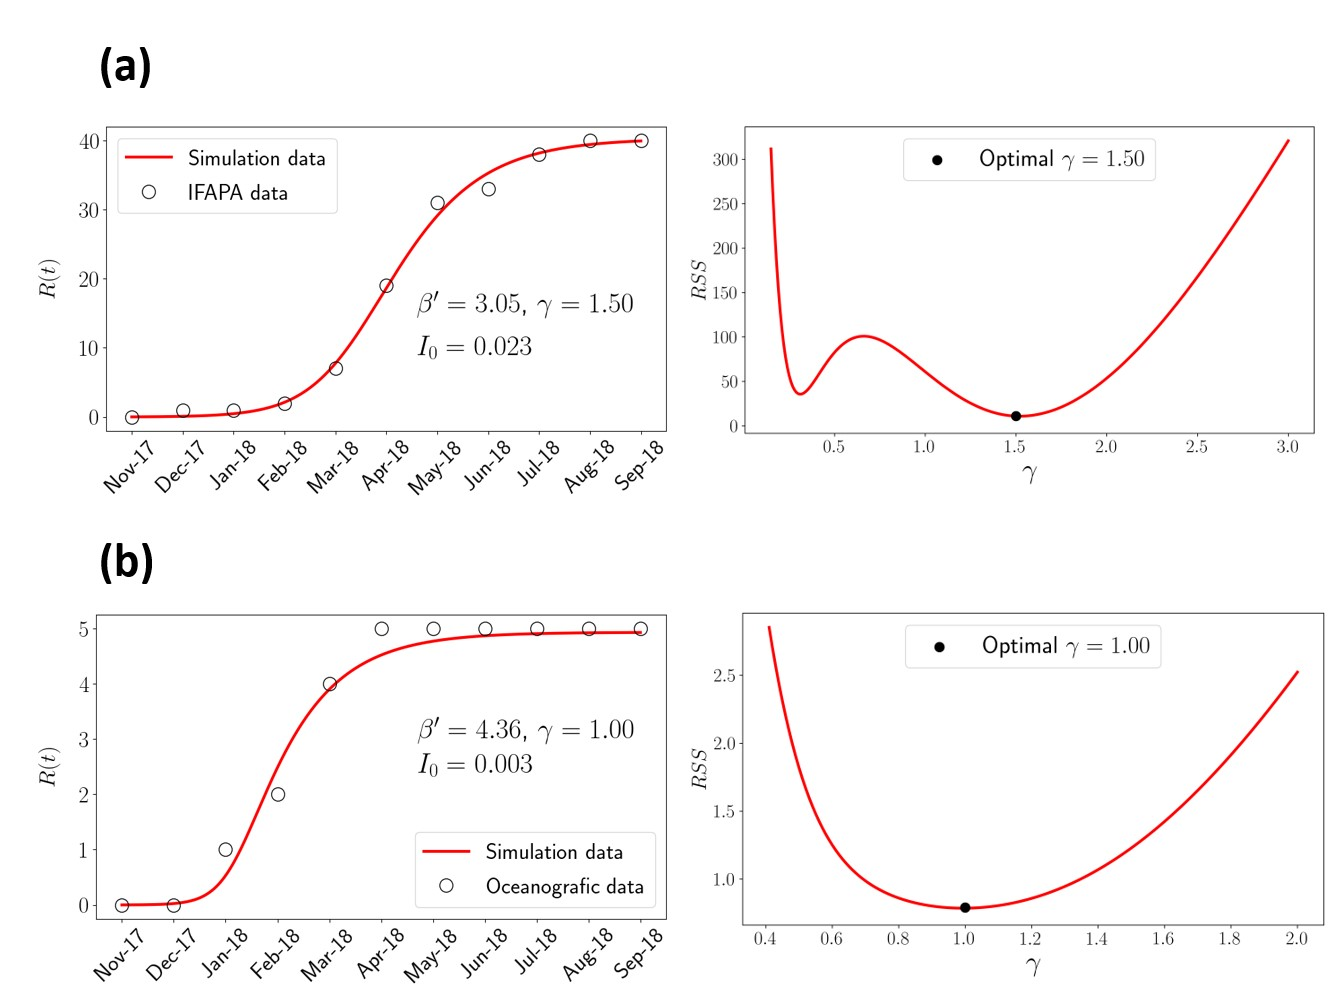
\includegraphics[width=1\textwidth]{Figures/approx_SIR_fitting.jpg}
    \caption{Parameter fitting for the R compartment to model
        (\cref{eq:SIRslow}) using data from IFAPA (panel (a)) and Oceanogràfic
        (panel
        (b)). The left part of both panels of the figure shows the optimal fit
        of the
        model to empirical data with $RSS=10.9, 0.8$ for IFAPA and OCE,
        respectively.
        The right panels show the variation of the $RSS$ error for some values
        of
        $\gamma$.  The $\beta'$ values have been obtained assuming a standard
        incidence, as explained in the main text.}
    \label{fig:approx_SIR_fit}
\end{figure}

Summarising, the SIRP model is able to fit two sets of experimental data,
agreeing with a standard incidence, according to which the infection rate
depends on the amount of parasites per pen shell individual. \textit{Pinna
    nobilis} individuals in
the IFAPA experiment were actually distributed in $4$ tanks, and the
standard incidence is compatible with this experimental aspect. The temperature
dependence of the fitted parameters in this range ($14-17 {}^o C$, appears to
be compatible (although experiments at different temperatures would be needed)
with an Arrhenius dependence of the infection parameters, also known as
Boltzmann-Arrhenius
\cite{Brown2004,Molnar2017}, that can be extended to account for the
expect unimodal dependence on temperature, with a maximum infectivity at a
characteristic temperature for the parasite \cite{Molnar2017}. Therefore, we
can assume that global change (or temperature shifts) is expected to have
complex effects on infectious diseases, causing some to increase, others to
decrease, and many to shift their distributions \cite{Rohr2020}.
In the particular case of pen shell mortality, our model results suggest the
proposed mechanism of lower disease expression at lower temperatures. This
might have direct consequences for the development of the mortality event and
offers a bleak perspective for the future and specifically in the eastern
Mediterranean basin, where the mortality was observed later due to current
patterns but average temperatures tend to be higher than in the western part of
the Mediterranean.

\section{Conclusions} \label{sec:conclusions}

In this work we have analysed a compartmental model to study marine epizootics
for sessile hosts assuming infection by direct transmission through waterborne
parasites. Moreover, we have used data from the recent mass mortality event of
\textit{Pinna Nobilis} in the Mediterranean Sea as a case study to validate our
model. Compartmental models are routinely used in the study of disease
infection and propagation in terrestrial ecosystems, including the study of the
current Covid-19 pandemic (see, e.g., \cite{Castro2020}). However, these
models are starting to be used only recently in the study of marine epizootics
\cite{article_SIP}, while proliferation models have been the most popular in
the field \cite{Powell2015}. A reason for
the low popularity of compartment models in the study of marine epizootics is
that there are some aspects in its modelling that differ from the now standard
application to terrestrial ecosystems \cite{MCCALLUM_intro}. An important
difference is that, in principle, (micro)parasites need to be modelled
explicitly in marine ecosystems, while often they are not included in the
description in terrestrial ecosystems  \cite{May1979}.

The SIRP model has $4$ compartments and depends on $4$ parameters, so that it
is not quite amenable to theoretical analysis. At the same time, due to the
large number of parameters of the model, using it to analyse experimental
observations can be cumbersome in practice if the parameter values are unknown.
Nevertheless, we have shown three reductions of the model, one exact and two
approximate ones, that can be useful to overcome these limitations that are
typically present at the first stages of emergent epidemics. Indeed, the
timescale approximation is able to fit the collected data of our case study for
some optimal parameters, as shown in \cref{sec:validation}. This approximation
is particularly useful as it only depends on $2$ parameters, the death rate of
infected hosts, $\gamma$ and an effective infection rate, $\beta'$. Although
this approximation simplifies the fitting procedure, there is a price to be
paid in this analysis. The infection parameter, $\beta$, and the parameters
regulating proliferation, $\lambda$, and deactivation/dilution of the parasite,
$\mu$, become entrained into a single effective parameter, $\beta'$. Thus, the
full understanding of the different effects at play in the system requires
further work. Furthermore, we have shown that an epidemic model for immobile
hosts can be reduced to the standard SIR model, which assumes direct contact
among the hosts, i.e. that the hosts are mobile. This reduction is only valid
when the time scale of the parasites is much faster than that of the hosts,
i.e. $\mu\gg\beta N,\gamma$. Thus, our work provides a ground to apply the SIR
model in marine epidemics of sessile hosts that fulfil the required conditions.

In a world with many possible new epizootics, we believe that our reduced model
can be specifically useful to understand key features of those emerging
diseases characterised by the spreading of waterborne parasites in a relatively
fast way, provided that the temporal evolution of the disease can be determined
for, at least, some set of individuals. Thus, some of the key parameters can be
fitted to the available experimental data as shown in \cref{{sec:validation}}.
Still, the fitted relevant parameters may need to be supplemented with further
information or targeted experiments. We hope that this approach can be useful
in understanding emerging diseases in shellfish species of economic not only
ecological value, and also, with suitable modifications, in aquaculture. It is
noteworthy that our case study is a haplosporidan waterborne parasite.	In
fact, waterborne haplosporidans have been responsible for some of the most
significant and consequential marine disease epizootics on record and are
considered the major pathogens of concern for aquatic animal health shellfish
industries around the world \cite{Arzul2015}. The SIRP model is the simplest
model that one could think of having in mind its practical application, but
could be extended to incorporate further effects that are so far described in
an effective way.

\section{Appendix}

\subsection{Finding a conserved quantity for the SIRP model}
\label{app:P_exact}

Starting with the SIRP model,
\begin{equation}\label{eq:SIRP2}
    \begin{aligned}
        \dot{S} & =-\bar{\beta} P S                    \\
        \dot{I} & =\bar{\beta} P S-\gamma I            \\
        \dot{R} & =\gamma I                            \\
        \dot{P} & =\lambda I-\bar{\beta}P S -\mu P \ ,
    \end{aligned}
\end{equation}
from the $\dot{S}$ equation, $P$ can be written as follows,
\begin{equation}\label{eq:P_rel}
    P=-\frac{1}{\bar{\beta}}\frac{\dot{S}}{S} \ ,
\end{equation}
and summing up the equations for $\dot{S}$ and $\dot{I}$ the following
relation for $I$ is obtained
\begin{equation}\label{eq:I_rel}
    I=-(\dot{S}+\dot{I})/\gamma \ .
\end{equation}
Replacing \cref{eq:P_rel}, \cref{eq:I_rel} and the differential equation
for $\dot{S}$ in the $4$th differential equation in \cref{eq:SIRP2} one
obtains,
\begin{equation}
    \dot{P}=-{{\lambda}\over{\gamma}} (\dot{S}+\dot{I})+\dot{S}+
    {{\mu}\over{\bar{\beta}}}\ . {{\dot{S}}\over{S}}
\end{equation}
As $\dot{S}/S=d(\ln S)/dt$, all terms in the previous equation are exact
differentials with respect to time, and the equation can be integrated
yielding,

\begin{equation}
    P + \frac{\lambda}{\gamma}\parentesi{S+I}-S-\frac{\mu}{\bar{\beta}}\ln S=C
    \label{eq:conservedquantity}
\end{equation}
with the integration constant $C$,
that is a conserved quantity, i.e., it takes the same value at one time of
the dynamical evolution of the system.
$C$ is related to the initial conditions by,
\begin{equation}
    C = P(0)+\frac{\lambda}{\gamma}\parentesi{S(0)+I(0)} -
    \frac{\mu}{\bar{\beta}}\ln{S(0)} -
    S(0)=P(0)+\frac{\lambda}{\gamma}\parentesi{N-R(0)} -
    \frac{\mu}{\bar{\beta}}\ln{S(0)} - S(0)
    \label{eq:C_constant}
\end{equation}

It is possible to use \cref{eq:conservedquantity}-\cref{eq:C_constant} to
express one of variables as a function of the others, for example
the parasite concentration $P$ as,
\begin{equation} \label{eq:PSI_exact}
    P(S, I)=P(0)-\frac{\lambda}{\gamma}\left(S+I-N+R(0)\right)+
    \frac{\mu}{\bar{\beta}}\ln{\frac{S}{S(0)}} + S - S(0)\ ,
\end{equation}
or equivalently as,
\begin{equation}\label{eq:psrexact}
    P(S,R)=P(0) + \frac{\lambda}{\gamma}\claudator{R-R(0)+
        \frac{\mu\gamma}{\bar{\beta}\lambda}\ln{\frac{S}{S(0)}}} + S - S(0)
\end{equation}

From \cref{eq:conservedquantity}, it is easy to show that the SIP model
of Ref. \cite{article_SIP}, that differs from the SIRP model in that the
fourth equation is simplified to $\dot{P}=\lambda I-\mu P$, has as
exact conserved quantity,
\begin{equation}
    P + \frac{\lambda}{\gamma}\parentesi{S+I}-\frac{\mu}{\bar{\beta}}\ln
    S={\mathcal C}
    \label{eq:conservedquantitySIP}
\end{equation}
as the extra term in the SIRP model $-\bar{\beta}SP$ is equal to $\dot{S}$
from the first equation \cref{eq:SIRP2}.

The SIR model has a conserved quantity \cite{Murray_book}, that in the case
of
\cref{eq:SIRslow} takes the form,
\begin{equation}
    I+S-{{\gamma}\over{\beta'}} \ln S =C\ .
    \label{eq:SIRconservedquantity}
\end{equation}
Rewriting \cref{eq:conservedquantity} in the alternative form,
\begin{equation}
    {{\gamma}\over{\lambda}} P +\left(1-{{\gamma}\over{\lambda}}\right) S + I
    -{{\mu\gamma}\over{\lambda\bar{\beta}}} \ln S=C'
    \label{eq:conservedquantity2}
\end{equation}
it can be seen that if $\lambda>>\gamma$ \cref{eq:conservedquantity2} reduces
to
\cref{eq:SIRconservedquantity}, remembering that in \cref{eq:SIRslow}
$\beta'=\lambda\bar{\beta}/\mu$. The assumptions used to arrive to
\cref{eq:SIRconservedquantity} in \cref{sec:fastslow} where
$\mu>>(\gamma,\bar{\beta})$, and taking into account the expression for $R_0$
\cref{eq:R_0_SIRP}, that $\lambda\gtrsim\mu$ is most plausible to keep $R_0$
above the epidemic threshold ($R_0>1)$.

\subsection{Stability analysis of the fixed points of the SIRP model}
\label{app:linstabfp}

Here we will assume the initial fixed point of our SIRP model, with
$I(0)=P(0)=0$ right before the introduction of the infection, either through
$I$ or $P$.
We will assume that $R(0)=0$, so that $S(0)=N$.
To study the linear stability of the model we need to write the Jacobian, that
takes the form,
\begin{equation}
    J=
    \begin{pmatrix}
        -\bar{\beta} P & 0       & 0 & \bar{\beta} S       \\
        \bar{\beta} P  & -\gamma & 0 & \bar{\beta} S       \\
        0              & \gamma  & 0 & 0                   \\
        -\bar{\beta} P & \lambda & 0 & (\bar{\beta} S-\mu)
    \end{pmatrix}
\end{equation}
and obtain the eigenvalues for both fixed points, where we have already used
the standard incidence, $\bar{\beta}=\beta/N$, from the evidence of the
validation with experiments.
For the pre-epidemic fixed point, the Jacobian becomes,
\begin{equation}
    \begin{pmatrix}
        0 & 0       & 0 & \bar{\beta} S(0)       \\
        0 & -\gamma & 0 & \bar{\beta} S(0)       \\
        0 & \gamma  & 0 & 0                      \\
        0 & \lambda & 0 & (\bar{\beta} S(0)-\mu)
    \end{pmatrix}
    \label{eq:Jacobian}
\end{equation}
Matrix \cref{eq:Jacobian} has two null $(0$) eigenvalues and a pair of
eigenvalues given by,
\begin{equation}
    \Lambda_{1,2}=-{1\over 2}\left(\gamma+\mu+{{\bar{\beta}
                S(0)}}\pm\sqrt{\gamma^2+\mu^2+\left({{\bar{\beta}
                    S(0)}}\right)^2
        +{{2\mu\bar{\beta} S(0)}}-2\gamma\mu
        -{{2\gamma\bar{\beta} S(0)}}+{{4\lambda\bar{\beta} S(0)}}}
    \right)
\end{equation}
from which one can determine that the fixed point is unstable whenever
\begin{equation}
    \lambda\bar{\beta} S(0)>\gamma(\mu+\bar{\beta} S(0))
    \label{eq:eigenvineq}
\end{equation}
and stable if the inequality is reversed.
It can be easily shown that \cref{eq:eigenvineq} is equivalent to $R_0>1$, with
$R_0$ given by \cref{eq:R_0_SIRP}.

The final point of the epidemic,  $S(\infty)$, can be found by solving the
transcendental equation,
\begin{equation}
    \left({{\lambda}\over{\gamma}}-1\right)S(\infty)
    -\frac{\mu}{\bar{\beta}}\ln (S(\infty))=C
    \label{eq:sinftytreqn}
\end{equation}
where $C$ is determined from the initial conditions (\cref{eq:C_constant})
and $I(\infty)=P(\infty)=0$.
(\cref{eq:sinftytreqn}) has two roots, where $S({\infty})$ represents the
smallest one.

\subsection{Calculation of $R_0$ using the Next Generation Matrix
    method}\label{app:NGM}

The so called Next Generation Method (NGM) is a method to obtain $R_0$, the
basic epidemiological quantity that measures the number of secondary cases
produced by a typical infected individual during its entire period of
infectiousness in a completely susceptible population. It was discussed in
\ref{app:linstabfp} that $R_0$ is related to the largest non-zero eigenvalue,
say $\Lambda$, of the fixed point corresponding to the infection-free
equilibrium. An outbreak occurs when $\Lambda>0$ (or equivalently when $R_0>1$)
and the NGM is an ingenious method to obtain directly $R_0$ in a reduced linear
system.
In more concrete terms, within the NGM method $R_0$ is the dominant eigenvalue
of a suitably defined linear operator (a linear matrix in a suitable basis).
This operator is obtained from a decomposition of the Jacobian, $J$ of
the infected/infecting compartments (i.e. excluding susceptible and removed
compartments) in the form $J=T+\Sigma$, where $T$ is
the
\textit{transmission part}, that describes the production of new infections,
and $\Sigma$  the \textit{transition part}, that describes changes of
state (including death). Then, it can be proved \cite{Diekmann2010} that the
\textit{basic reproduction number} $R_0$ is given by the spectral radius (i.e.
the largest eigenvalue) of the (next generation) matrix $K=- T
    \Sigma^{-1}$.

In the case of the SIRP model the decomposition is applied to the $2\times 2$
Jacobian corresponding to the dynamical evolution of the $(I,P)$
\textit{infectious} compartments, being the decomposition,
\begin{equation*}
    J=\parentesi{\begin{array}{cc}
            -\gamma & \bar{\beta} S_0        \\
            \lambda & -(\bar{\beta} S_0+\mu)\end{array}}\qquad
    T=\parentesi{\begin{array}{cc}
            0 & \bar{\beta} S_0 \\
            0 & 0
        \end{array}} \qquad \Sigma=\parentesi{\begin{array}{cc}
            -\gamma & 0                        \\
            \lambda & -(\bar{\beta} S_0 + \mu)
        \end{array}}
\end{equation*}
where the $\bar{\beta} PS$ term in $\dot{I}$ is the only one that contributes
to the transmission matrix, as it is the only process involving infection,
while all the other terms in the dynamical equations of $\dot{I}$ and $\dot{P}$
imply transitions (to another compartment, like $I\rightarrow R$ or birth and
death of $P$).

Then, the next generation matrix is given by,
\begin{equation*}
    K=- T\Sigma^{-1}=\parentesi{\begin{array}{cc}
            \displaystyle \frac{\lambda\beta S_0}{\gamma(\beta S_0 + \mu)} &
            \displaystyle \frac{\beta S_0}{\beta S_0 + \mu}
            \\
            0                                                              & 0
        \end{array}} \Longrightarrow R_0=\frac{\lambda \beta
        S_0}{\gamma\parentesi{\beta S_0+\mu}} \ ,
\end{equation*}
This result coincides with the expectation that $R_0$ should correspond to the
number of  hosts infected in a single generation by the appearance of an
infected host in a completely susceptible population. This can be obtained from
the number of parasites produced by an infected host, $\lambda$, times the time
in which the infected host is alive producing parasites, $1/\gamma$, multiplied
by the number of infected hosts produced per parasite, $\beta S_0$, times the
time the parasite is alive available to infect, $1/(\mu+\beta S_0)$, taking
into account that parasites are inactivated at a rate $\mu$ and also die when
infecting at a rate $\beta S_0$, where this result assumes that the susceptible
population does not change from its initial value $S_0$.

\subsection{Sensitivity Analysis} \label{app:sensanal}

One particular way to analyse the local sensitivity (LSA) of a given model
function, $F(\vec{p})$, for each of the parameters that conform it, $p_i$, is
through the normalised sensitivity indexes \cite{sensitivity_analysis},
\begin{equation}\label{eq:sensitivity_analysis}
    \Omega_{p_i}^{F}=\dpart{F}{p_i}\frac{p_i}{F}\Big|\limitss{p_i=p^0}{} \
    .
\end{equation}
where the partial derivatives in \cref{eq:sensitivity_analysis} are
determined analytically in our case.

GSA works by studying the influence of a large domain of parameter space in
the final state of the epidemic and in the epidemic peak.
In our case this will be achieved by means of a variance based analysis,
known as Sobol method \cite{SOBOL2001271}. This particular method provides
information no only on how a particular parameter alone influences the model
outputs (as happens with LSA), but also on the influence of its interactions
with other parameters. This information is organised in what are known as Sobol
indices, that have been
implemented within the Julia high-level programming language \cite{julia}
using the DifferentialEquations.jl package \cite{DifferentialEquations.jl},
and in particular through its subpackage DiffEqSensitivity.jl. This
implementation allows the user to sample the parameter space using
QuasiMonteCarlo methods and thus obtain confidence intervals (CI) for the
sensitivity indices, which are directly related to the committed statistical
error.

The total order indices are a measure of the total variance of the output
quantity caused by variations of the input parameter and its interactions.
First order (or ``main effect'') indices are a measure of the contribution to
the output variance given by the variation of the parameter alone, but averaged
over variations in other input parameters. Second order indices take into
account first order interactions between parameters. Further indices can be
obtained, describing the influence of higher-order interactions between
parameters, but these are not going to be considered.
More detailed information about sensitivity analysis can be found in
\cite{Sensitivity_analysis_book}.

\subsection{General rate change with temperature} \label{app:rate_change}

In \cite{Gillooly2248} the metabolic rate of a wide variety of organisms
was studied, showing that the change in the metabolic rate with temperature was
similar among them. In particular, the natural logarithm of the metabolic rate
linearly depends on the inverse of absolute temperature,
\begin{equation}
    \log(R(T))=a\cdot\parentesi{\frac{100}{T}}+b
\end{equation}
and for all the analysed organisms they found that $a$ lies between $-5$
and $-10$ and $b$ between $14$ and $30$. From their analysis, we can compute
the change in the rate for a given increase of temperature,
\begin{equation}\label{eq:rate_change}
    \frac{R(T+\Delta T)}{R(T)}=\exp(a\cdot\parentesi{\frac{100}{T + \Delta
            T}}+b) / \exp(a\cdot\parentesi{\frac{100}{T}}+b) = \exp(a \cdot
    \frac{-1000}{T+\Delta T}\cdot \frac{\Delta T}{T}) \ .
\end{equation}
Substituting $T=287 K$ and $\Delta T=3 K$, that correspond to our available
data (cf. \cref{sec:validation}) in \cref{eq:rate_change}, using both the upper
and lower limit of $a$, we obtain that the expected increase in the effective
transmission rate is between $1.2$ to $1.4$. This is far from the $19$-fold
increase that we obtained with the mass action hypothesis in
\cref{sec:validation}
while it is in good agreement with either the $1.92$ ratio we obtained	for
$\bar{\beta}$ with the reduction of \cref{sec:exactredapp} or the $1.43$ ratio
obtained with the fast-slow approximation of \cref{sec:fastslow}, both obtained
using the standard incidence choice.

\cref{fig:rate_changes}(a) shows the change in the rate with an increase of
$\SI{3}{\degree C}$ for different base temperatures and for all the organisms
analysed in \cite{Gillooly2248}, and using their fit. Note that for all
temperatures between $\SI{0}{\degree C}$  and $\SI{30}{\degree C}$ the rate
change lies between $1.2$ and $1.45$. \cref{fig:rate_changes}(b) shows the
change in the rate for different temperature increases, with a base temperature
of $T=\SI{287}{K}$. Note that in order to obtain a $19$-fold increase the
temperature change should be at least of $\SI{30}{\degree C}$\footnote{A
    temperature change of $\SI{30}{\degree C}$ could fall outside the range in
    which the study of \cite{Gillooly2248} is valid. We just stress that a
    $19$-fold rate change is unlikely for the case of a $\SI{3}{\degree C}$
    that
    correspond to the $2$ data sets that we compare in this section.}.
The temperature dependence of metabolic rates has been reported in the
context of epidemic parameters \cite{COELHO2006,Shapiro2017}

The behavior of the metabolic rates re-analysed here has been also found
experimentally in epidemic contexts such as \cite{COELHO2006, Shapiro2017},
i.e. the increase of the rates with temperature fulfill the ranges shown here.

\begin{figure}[H]
    \centering
    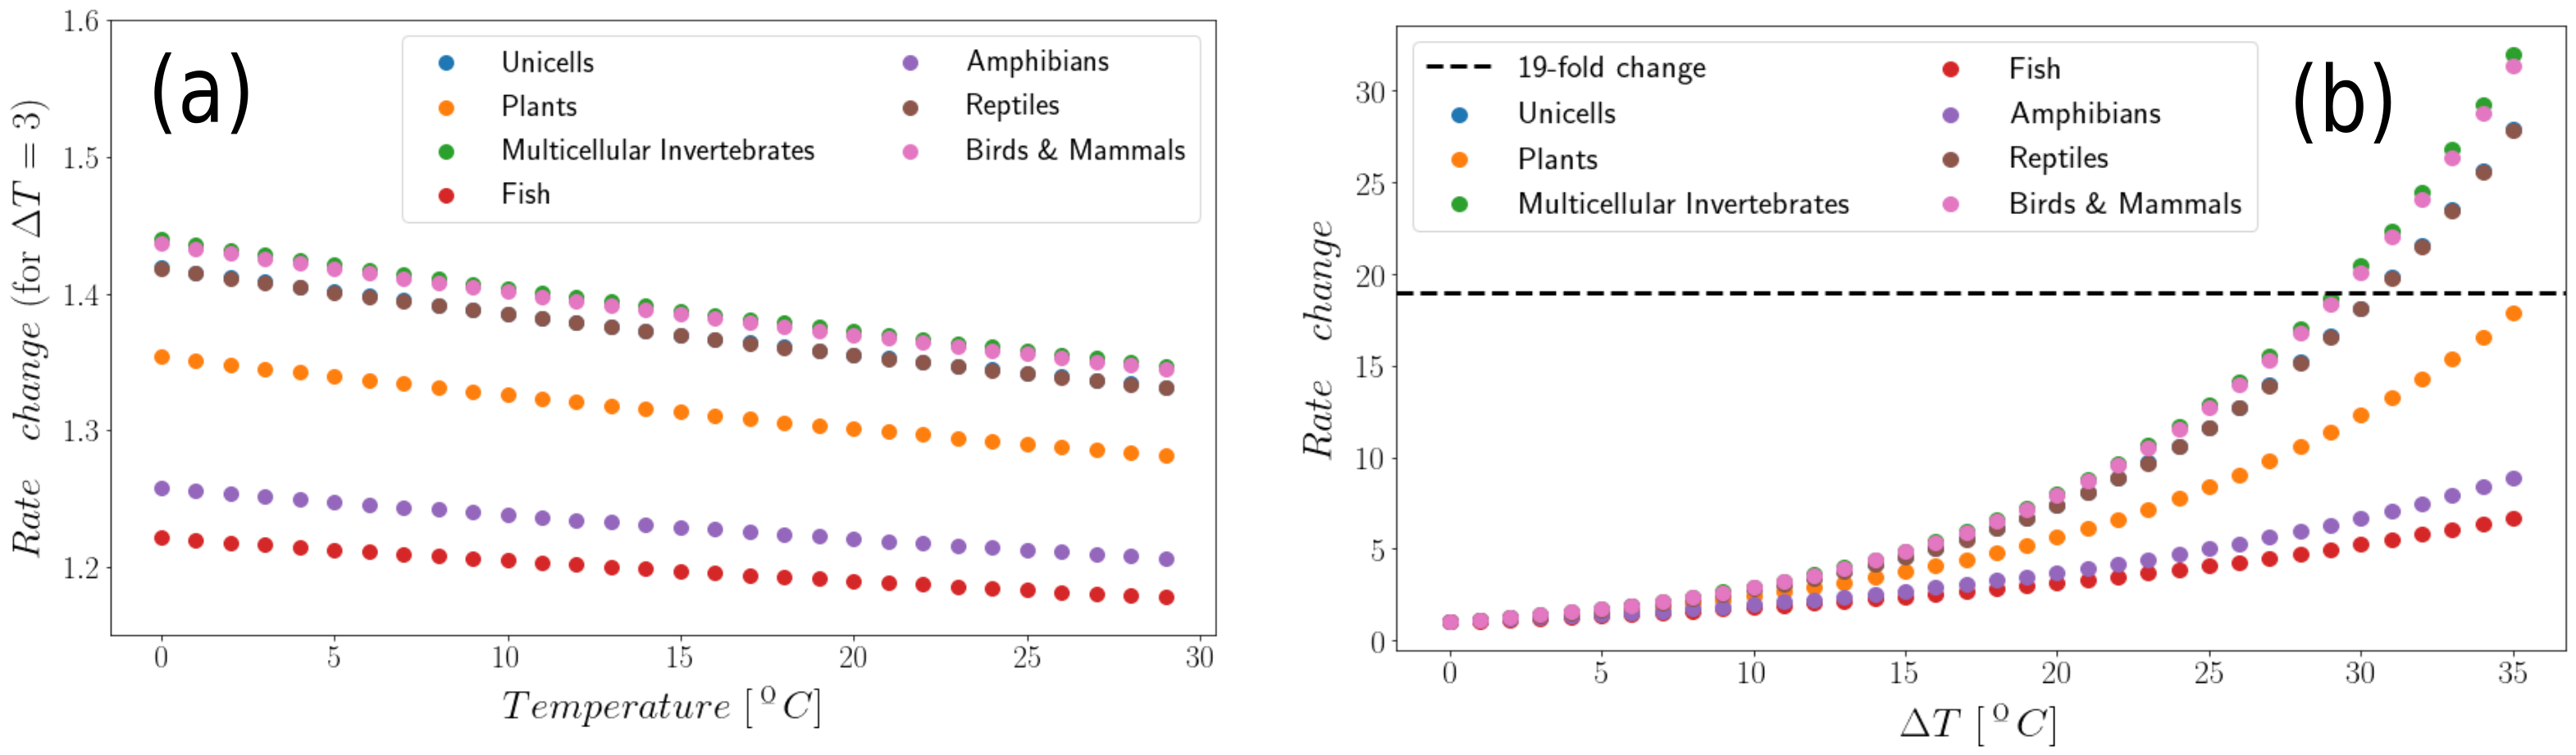
\includegraphics[width=1\textwidth]{Figures/arrhenius.png}
    \caption{Graphical representation of change in the rate (in ordinates)
        for different reference temperatures (in abscissae) for: (a) a
        temperature
        increase of $\SI{3}{\degree C}$; (b)  a temperature increase of
        $\SI{14}{\degree C}$. The black dotted line in (b) corresponds to a
        $19$-fold
        increase in the rate.
    }
    \label{fig:rate_changes}
\end{figure}

%----------------------------------------------------------------------------------------
%	Spatial effects in parasite-induced marine diseases of immobile hosts
%----------------------------------------------------------------------------------------
\chapterimage{nacra2.png}
\chapterspaceabove{6.75cm}
\chapterspacebelow{7.25cm}

\chapter{Spatial effects in parasite-induced marine diseases of immobile hosts}
\vspace{3cm}

% \begin{center}
%     \textbf{Àlex Giménez-Romero$^{1}$, Federico Vázquez$^{2,1}$, Cristóbal
%         López$^{1}$, Manuel A. Matías$^{1}$}
% \end{center}

% \vspace{1cm}

% \begin{enumerate}
%     \small
%     \item Instituto de Física Interdisciplinar y Sistemas Complejos, IFISC
%           (CSIC-UIB), Palma de Mallorca 07122, Spain
%     \item Instituto de Cálculo, FCEyN, Universidad de Buenos Aires and CONICET,
%           Buenos Aires, Argentina

% \end{enumerate}

% \vspace{1cm}

\textbf{Published as}

\vspace{0.5cm}

\fullcite{GimenezRomero_2022_RSos_e}

\newpage
\section{Introduction}

Wildlife emergent infectious diseases represent a substantial threat to
ecosystems and the conservation of their biodiversity \cite{Daszak443}. Their
effects can be devastating at the ecological level, causing local extinctions
\cite{Daszak443} and in some cases pushing endemic species to the verge of
extinction, as is the case of \textit{Pinna nobilis}
\cite{Cabanellas2019}; at the economic level, producing losses in agriculture,
livestock and aquaculture \cite{Vurro2010, Tomley2009, Pernet2016}, and impact
human health, as is the case of the COVID-19 pandemic \cite{Salata2020}. For
the past decades, parasites have been continuously emerging \cite{Morens2004,
    Daszak2017}, while globalisation and climate change have contributed to
their
evolution. This has allowed these parasites to enter in new ecological niches
and spread further the diseases they produce \cite{Aguirre2008}. In particular,
marine infectious diseases are recently increasing due to these and other
anthropogenic pressures, like pollution and overfishing \cite{Lafferty2004},
inducing widespread mass mortalities in several species \cite{Eisenlord2016,
    JONES201648, VAZQUEZ2017}.

An important subset of marine organisms affected by infectious diseases are
sessile (i.e. they cannot move), like bivalves, sponges or corals. An
increasing number of outbreaks affecting marine mollusks have been reported,
some of them causing mass mortalities in commercially important bivalves
\cite{Guo2016}. Mainly due to the economic importance of some species (e.g.
oysters), infectious diseases in bivalve populations have been deeply studied
\cite{Petton2021, Pernet2018, McLaughlin2005, powell1999modeling}. Recently,
deterministic compartmental models have been used to describe parasite
transmitted diseases in marine sessile bivalves \cite{BIDEGAIN_2016_2,
    BIDEGAIN_perkinsus, GimenezRomero2021}, showing to be able to accurately
predict disease transmission in some circumstances. The main limitation of
these compartmental models is the assumption of a non-spatial description of
the system under study. This underlying hypothesis assumes that any pair
parasite-host of the system can interact at any time, which is unrealistic in
general. A non-spatial description assumes well mixed populations, which
implies that the mean distance among hosts is smaller than the the typical
distance explored by parasites in their lifetime. This assumption can be quite
realistic in some situations, as it is in \cite{GimenezRomero2021} where the
hosts were kept in tanks with water renovation. However, a non-spatial model is
not expected to yield a good description of spatially extended hosts in a
natural setting.

The key quantity in mathematical epidemiology is the basic reproductive number,
$R_0$, that represents the number of infected individuals generated in one
generation by the appearance of a single infected individual in a fully
susceptible population. Thus, $R_0>1$ ensures the onset of an epidemic, as the
number of infected individuals will grow exponentially	producing a widespread
disease \cite{Anderson1991}. If we first disregard spatial effects and assume a
non-spatial description, $R_0$ can be obtained from standard methods, like the
Next Generation Matrix method \cite{Diekmann2010}, and will only depend on
\textit{intrinsic} characteristics of the pathosystem (host-pathogen system)
under study. However, this basic reproduction number is unable to characterise
the threshold behaviour in many situations, including spatially extended
systems \cite{Cross2007, Li2011, RILEY201568}. In these systems, the
propagation of an epidemic to the entire system needs that a certain spatial
threshold is exceeded \cite{Gilligan2008}. Otherwise the disease will only take
place in suitable localised parts of the system, not being able to propagate to
the total system. Thus, disease spread will be strongly affected by the host
spatial distribution and pathogen mobility, which are not accounted for in
non-spatial models.

In this work we will try to unravel the transmission mechanisms of a
parasite-induced disease affecting immobile hosts in a spatially extended
system. We will approach the problem both theoretically and through numerical
simulation. The numerical study is based on Individual-Based Modelling (IBM), a
method widely used to study ecological systems \cite{Grimm2005}, so that
individuals are treated as discrete entities, space is introduced explicitly
and the dynamics are stochastic. Representative average behaviours can be
obtained by averaging over a sufficient number of realisations, and the
accuracy of the approach can be calibrated by deriving the corresponding
non-spatial limit, that can be confronted with the suitable compartmental model
on which a particular IBM is based. The IBM approach to our problem will allow
to study in depth the relation between pathogen mobility and immobile host
infection. As parasites move randomly over the space, tracking the position of
each parasite at different times turns to be of fundamental importance to
properly capture the stochastic dynamics of infections from parasites to hosts.
Modelling parasites and hosts as individual entities allows to take into
account the spatial and temporal heterogeneity of interactions between them.
This heterogeneity and the level of control in microscopic interactions cannot
be captured by other mathematical approaches such as partial differential
equations. On the other hand, IBMs are mathematically involved, and analytical
treatments are normally cumbersome, while their numerical implementation is
computationally expensive \cite{Breckling1900}.

Here we introduce a spatially-explicit individual-based model to study
parasite-induced marine diseases of immobile hosts. The model is applied  to
the case of diffusing parasites and uniformly distributed hosts. The system
under study is an extension of the compartmental model presented in
\cite{GimenezRomero2021}. As a main result, we find that the occurrence of an
outbreak will depend on the balance between the intrinsic characteristics of
the pathosystem, well represented by the above described non-spatial basic
reproductive number, $R_0$, and features that characterise parasite mobility.
We generalise the basic reproductive number, that we will refer to as
$\tilde{R}_0$, such that it accounts for the number of hosts that get infected
by the appearance of a single infected individual in a fully susceptible
population in a spatially extended system. $\tilde{R}_0$ characterises the
global epidemic and can be written as a product between $R_0$ and a factor
describing parasite mobility. The latter factor is smaller and at most equal to
$1$, which implies that, as it could be expected, it is more difficult to
induce a global outbreak in a spatially extended system (a two dimensional
lattice in our case) that in a well mixed (non-spatial) population.

% The paper is organised as follows: in \cref{sec:model}, we introduce some
% biological considerations for bivalve epidemics, discussed in more detailed in
% Ref. \cite{GimenezRomero2021}, and build the spatially-explicit model. In
% \cref{sec:results}, we present analytical results that are discussed and
% supported by numerical simulations. Specifically, the high mobility limit is
% discussed and connected to the the compartmental model. An approximation for
% the parasite population is discussed. Then, the effect of parasite mobility to
% the epidemic threshold is characterised, deriving an analytical expression for
% the basic reproduction number. Furthermore, the spreading speed of the disease
% and the time-scale to extinction is investigated. Finally, \cref{sec:
%     conclusions} contains some concluding remarks.

\section{The SIRP spatial model} \label{sec:model}

The most important biological features of the system under study are as
follows. First, hosts are immobile, while the disease is transmitted by
parasites produced by infected hosts. There are two mechanisms by which
parasites are cleared from the medium: i) they have a finite life time after
which they die or get inactivated; ii) they get absorbed after they infect a
host and thus are no
longer in the medium and cannot infect other hosts. Recruiting (birth) of hosts
occur at a very slow rate compared to other timescales in the system, and
accordingly it will be considered negligible in the model. Moreover, hosts do
not show long-term immunity, as is typical of invertebrates, like mollusks
\cite{Powell2015}. We also assume that recovery (healing) of infected hosts, if
it occurs, can be neglected. Furthermore, we consider that dead hosts are not a
source of parasites in the medium. See \cref{ch:nacras_I}
\cite{GimenezRomero2021} for a detailed
presentation of the non-spatial SIRP model, including these biological
modelling considerations.

Under these considerations, we introduce an individual-based model with
explicit space characterisation to study the effect of parasite mobility in
disease transmission. We consider a square grid of length $L$ with periodic
boundary conditions and place a single host per site, so that there are $N=L^2$
hosts. The hosts can be in three discrete states: susceptible, $S$; infected,
$I$ and dead (or removed), $R$. Then, we introduce the parasite population as a
new individual with a single state, $P$. Hosts are sessile (i.e. immobile),
while parasites are allowed to move between the lattice sites. As initial
condition we assume that the entire host population is susceptible,
$S(0)=N=L^2$, and that a small initial number of parasites, $P(0)$ is
introduced in the system.

Infection occurs when susceptible hosts filter parasites in their close
proximity. Accordingly, the infection process is implemented between parasites
and susceptible hosts sharing the same lattice site. In particular, susceptible
hosts in contact with a parasite become infected at rate $\beta$. As the
infection event implies the filtering of a parasite by a susceptible host, when
a new infection occurs a parasite of that particular site is removed. Infected
individuals die at rate $\gamma$ and produce parasites at rate $\lambda$, while
parasites die at rate $\mu$. Parasites move randomly between the four
neighbouring lattice sites at rate $\kappa$, which corresponds to a diffusive
motion. \cref{tab:IBM_params} contains the definitions of the variables and
parameters of the model and \cref{fig:IBM} shows a schematic representation of
the dynamics.

\begin{figure}[H]
    \centering
    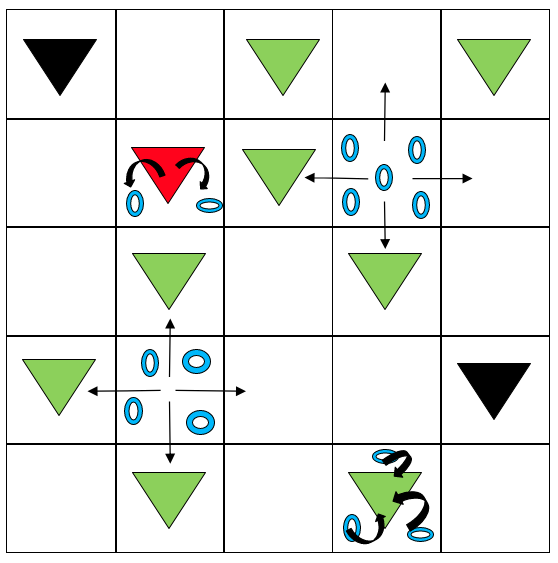
\includegraphics[width=0.6\textwidth]{Figures/IBM.png}
    \caption[Scheme of the individual based SIRP model]{Scheme of the
        individual based model. Green, red and black
        triangles represent susceptible, infected and dead hosts, respectively.
        Blue
        rings represent parasites, which move randomly between cells.
        Susceptible hosts
        get infected by filtering parasites while infected hosts produce them.
        Dead
        hosts do not participate in the dynamics of the system.}
    \label{fig:IBM}
\end{figure}

\begin{table}[H]
    \centering
    \caption[Variables and parameters of the individual based SIRP
        model]{Variables and parameters of the individual based SIRP model.}
    \resizebox{0.8\columnwidth}{!}{
        \begin{tabular}{cl}
            \hline \hline
            \textbf{Variable/Parameter} & \textbf{Definition}
            \\ \hline
            S                           & Susceptible host
            \\
            I                           & Infected host
            \\
            R                           & Dead host
            \\
            P                           & Parasite
            \\
            $\beta$                     & Parasite-host transmission rate
            \\
            $\gamma$                    & Host mortality rate
            \\
            $\lambda$                   & Production rate of parasites by
            infected hosts
            \\
            $\mu$                       & Parasite natural death rate
            \\
            $\kappa$                    & Parasite dispersal rate (mobility)
            \\
            $R_0$                       & Non-spatial basic reproductive number
            \\
            $\tilde{R}_0$               & Spatial basic reproductive number
            \\ \hline \hline
        \end{tabular}
    }
    \label{tab:IBM_params}
\end{table}

Formally, the model is mathematically described by a system of $N$ master
equations for the probabilities of the states in each lattice site $i$.
\cref{eq:scheme} summarises the reactive events. This is
very difficult to manage analytically, so the time evolution of the model is
numerically solved using Gillespie's algorithm \cite{Gillespie1977} (the code
can be found in \cite{CODE_nacras}).
\begin{equation}\label{eq:scheme}
    S+P \stackrel{\beta}{\rightarrow} I + \varnothing \quad I
    \stackrel{\gamma}{\rightarrow} R \quad I \stackrel{\lambda}{\rightarrow}
    I+P
    \quad P \stackrel{\mu}{\rightarrow} \varnothing
\end{equation}

\section{Results}\label{sec:results}
In this section several features of the model are studied, both numerically
(from IBM simulations) and analytically. All numerical results were obtained
for a square lattice of length $L=100$, with $N=S(0)=10^4$ hosts and using a
small initial condition of $P(0)=50$ parasites in the centre site.

\subsection{Non-spatial limit} \label{sec:MFlimit}
An important test of the IBM implementation is to show that, under suitable
circumstances, it converges to the non-spatial model on which the IBM is based.
This occurs in the limit when the parasites move many times before dying or
infecting a susceptible host. In this situation, each parasite typically visits
all the hosts of the system and may infect any of them. This is equivalent to
infecting a random host of the system, which happens with probability $\beta
    S/N$, being $S$ the total number of susceptible hosts in the system.
This corresponds to standard incidence, which represents the most accurate
description of the infection process
(\cref{ch:nacras_I},\cite{GimenezRomero2021}).
An equivalent picture is that parasites will end up uniformly distributed in
the lattice, so that there will be $P/N$ parasites in each lattice site at any
time. One expects to reach these conditions when $\kappa\gg\mu,\beta$, and,
thus the system as a whole can be described by the following system of ordinary
differential equations (ODE's),
\begin{equation}\label{eq:SIRP_MF}
    \begin{aligned}
        \dot{S} & =-\beta P S/N \, ,               \\
        \dot{I} & =\beta P S/N-\gamma I \, ,       \\
        \dot{R} & =\gamma I \, ,                   \\
        \dot{P} & =\lambda I-\beta P S/N-\mu P \ ,
    \end{aligned}
\end{equation}
that is precisely the SIRP non-spatial model \cite{GimenezRomero2021}, where
$S$, $I$, $R$ are the total number of susceptible, infected and recovered hosts
in the system, $P$ the total number of parasites and $N$ is the number of
hosts.

The basic reproduction number, $R_0$, of this non-spatial model is the
dimensionless quantity that yields the number of secondary infections generated
by the appearance of a single infected individual in a completely susceptible
population, also indicating whether the system will exhibit an epidemic
outbreak, $R_0>1$, or not, $R_0<1$.
In our case it can be directly computed as the mean number of parasites
produced by an infected host during its mean lifetime, $\lambda/\gamma$, times
the mean number of susceptible hosts that get infected by parasites during
their mean lifetime, $\beta/(\mu+\beta)$,
\begin{equation}\label{eq:R0_MF}
    R_0=\frac{\lambda}{\gamma}\frac{\beta}{\mu+\beta} \ .
\end{equation}
This result can be corroborated with standard methods such as the Next
Generation Matrix method \cite{Diekmann2010} (see \cite{GimenezRomero2021}),
where $S(0)=N$ has been considered.

Moreover, the model has a conserved quantity $\mathcal{C}$
\cite{GimenezRomero2021} that allows to find an analytical expression for the
final number of dead individuals (\cref{app:Rinf}),
\begin{equation}\label{eq:R_inf}
    R(\infty)=N+\frac{S(0)}{\xi}W_0\parentesi{-\xi\exp(-\frac{\beta}{\mu}C)} \
    ,
\end{equation}
with $\displaystyle\xi=S(0)\frac{\beta\parentesi{\lambda-\gamma}}{\mu\gamma}$
and $\displaystyle C=P_0+\frac{\lambda}{\gamma}\parentesi{S(0)+I(0)}-S(0)$.

The non-spatial limit of the model has been evaluated by comparing realisations
of the stochastic model (in the limit $\kappa\gg\mu,\beta$) with numerical
solutions of the non-spatial ODE system of \cref{eq:SIRP_MF}. Furthermore, the
analytical expression for $R(\infty)$ using the non-spatial model,
\cref{eq:R_inf}, is also compared to the numerical results of the individual
based model. As shown in \cref{fig:MF_limit} (a)-(c), as $\kappa$ is increased
compared to $\mu$ the individual based model approaches the non-spatial one.
\cref{fig:MF_limit}(d) shows how the numerical results for $R(\infty)$ for
different $R_0$ values approach the analytical solution in the non-spatial
limit.

\begin{figure}[H]
    \centering
    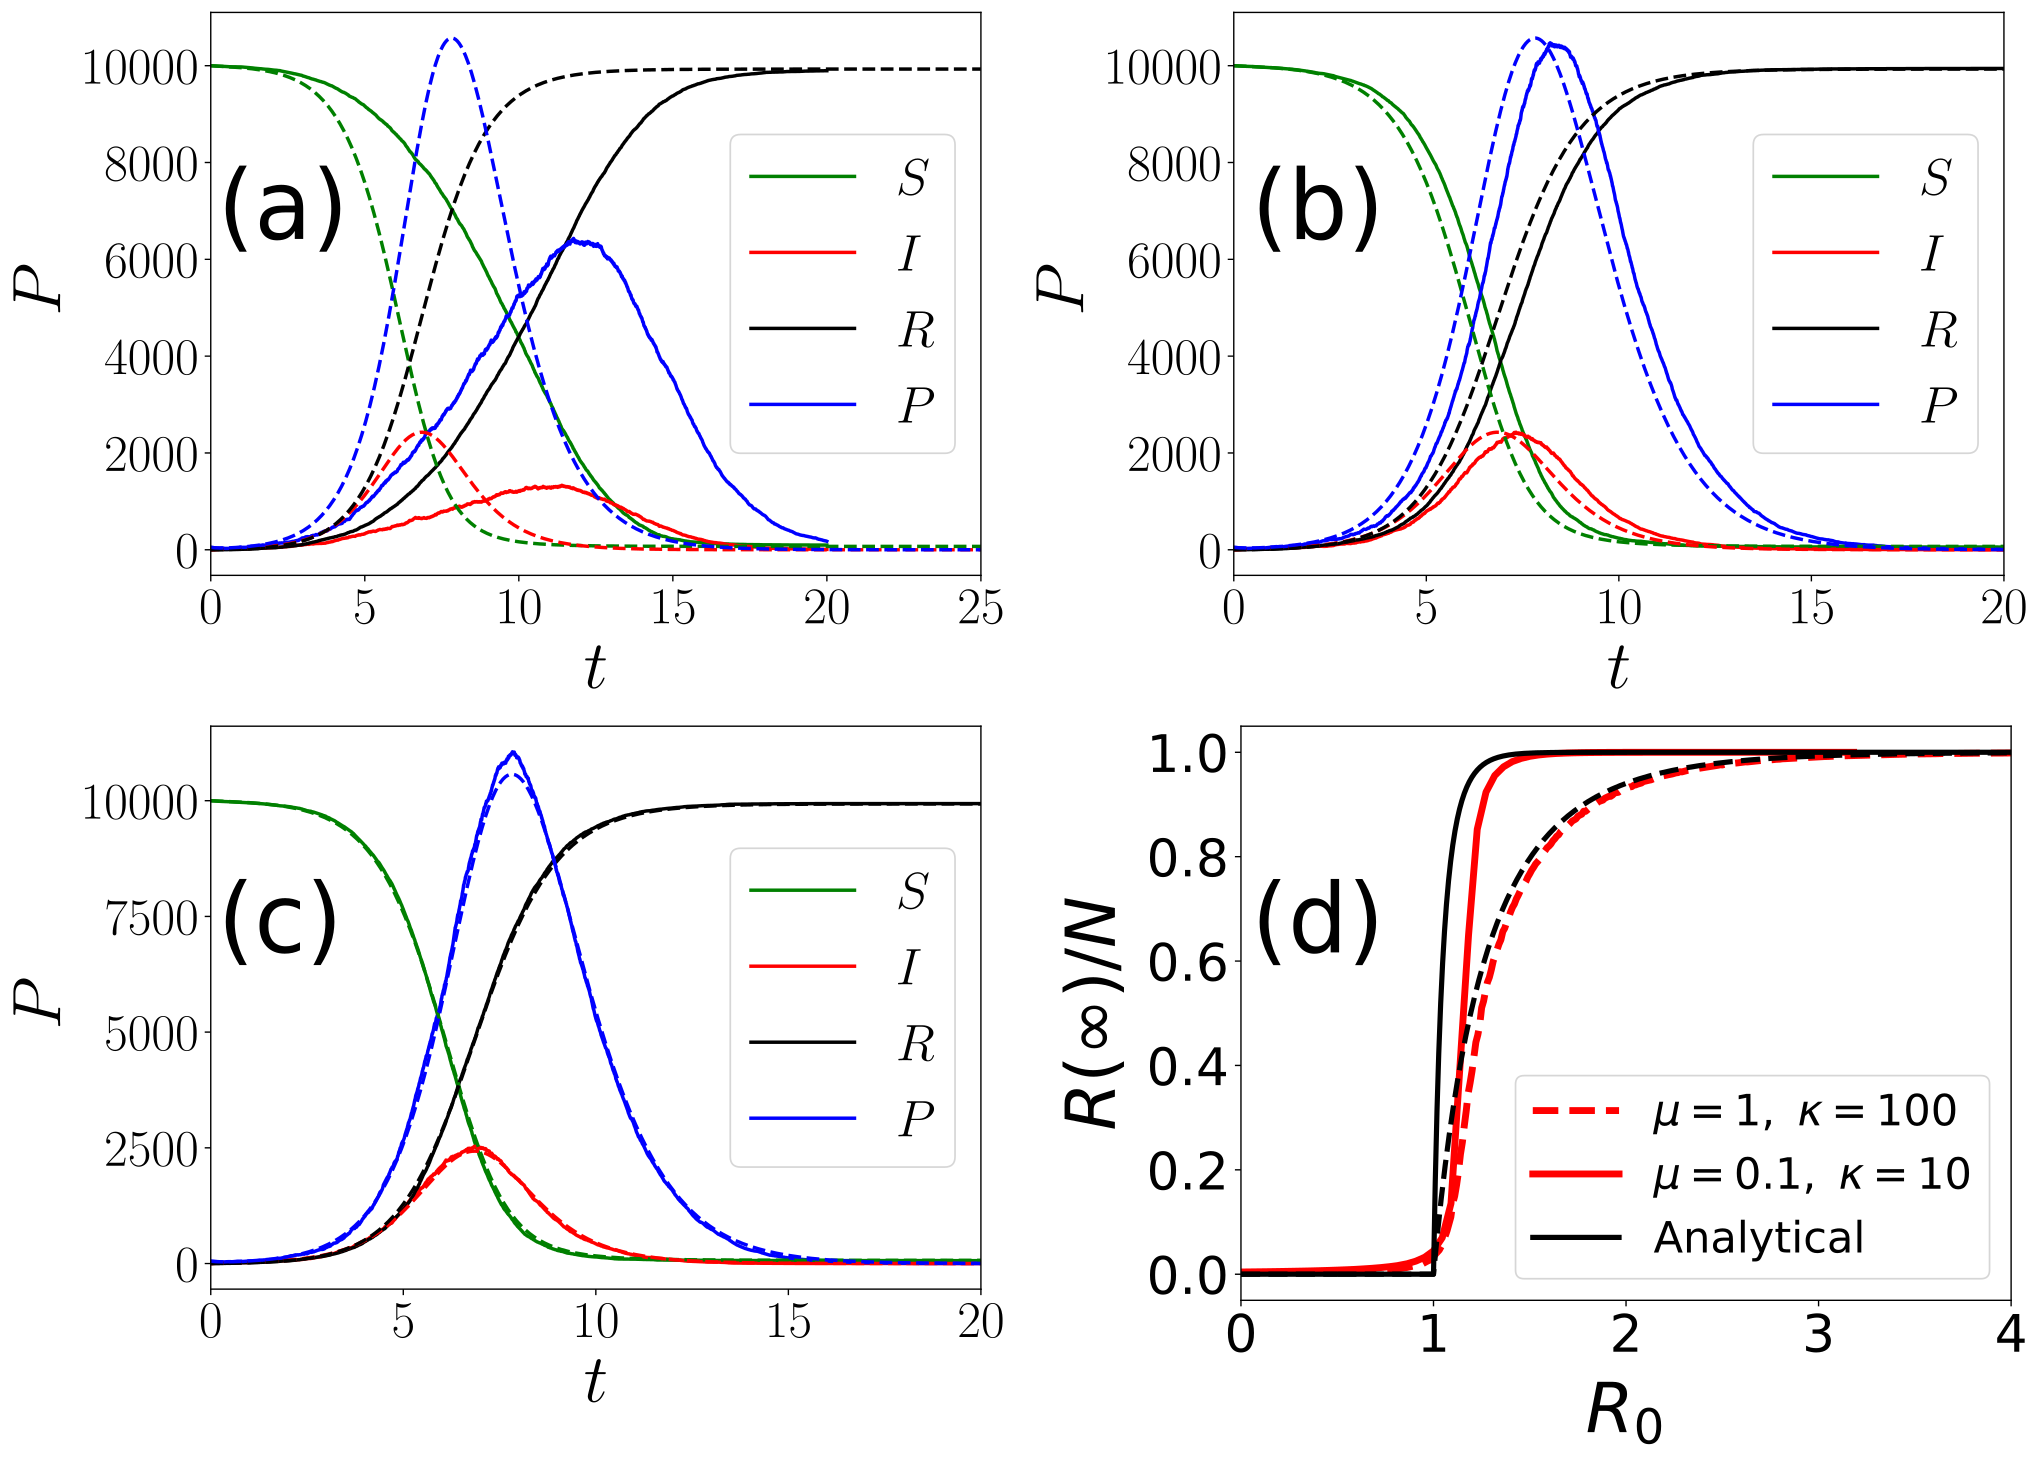
\includegraphics[width=\columnwidth]{Figures/MF_comparison.png}
    \caption[
        Comparison between the non-spatial model and the individual based model
        in the high mobility limit
    ]{Numerical solution of the non-spatial model (\cref{eq:SIRP_MF},
        dashed lines) compared with numerical solutions of the individual based
        model
        (solid lines) approaching the non-spatial limit with fixed
        $\gamma=\mu=\beta=1$
        and $\lambda=6$. (a) $\kappa=10^2$, (b) $\kappa=10^3$, (c)
        $\kappa=10^4$. Panel
        (d) shows the final fraction of dead hosts, $R(\infty)/N$, as function
        of $R_0$
        for $\kappa/(\mu+\kappa)=0.999$ with $\mu=1,0.1$ compared to the
        analytical
        result.}
    \label{fig:MF_limit}
\end{figure}

\subsection{Approximate relation between parasites and infected hosts}

In the limit $\kappa\gg\beta,\mu$ a time-scale approximation can be
performed so that the parasite population dynamics directly relates to that of
the infected hosts. In the non-spatial limit it was already shown in
\cite{GimenezRomero2021} that, if  $\mu\gg\beta,\gamma$ and $\lambda\gg\beta
    P/N$, the total parasite population of the system can be well described
using
the approximation (see \cite{GimenezRomero2021} for a detailed discussion),
\begin{equation}\label{eq:P_approx_II}
    P(t)\approx \frac{\lambda}{\mu} I(t) \ .
\end{equation}

Here we extend the validity of this approximation to spatial systems far
from the non-spatial limit. Consider the local dynamics of the parasite
population on a lattice site $i$. Note that when the host in the site is
susceptible, parasites in this site can either infect the host, die, or move to
another site. All these processes imply that a parasite will disappear from the
current site. Once the host at site $i$ gets infected, infection can no longer
occur whereas parasite production is now possible. If $\kappa$ is small enough
compared to $\lambda$ and $\mu$,  the only competing processes in sites with
infected individuals will be the production of parasites and their natural
death, which can be fairly described by the following rate equation,
\begin{equation}
    \der{P}{t}=\lambda-\mu P \ ,
\end{equation}
which solution is
\begin{equation}\label{eq:P_evol}
    P(t)=\frac{\lambda}{\mu}+\claudator{P(0)-\frac{\lambda}{\mu}}e^{-\mu t}
    \ .
\end{equation}

From \cref{eq:P_evol} one may notice that the stationary value of $P$,
$\lambda/\mu$, is reached in a time proportional to $t_{\textrm{eq}}\propto
    1/\mu$. This derivation allows to find a condition for which
\cref{eq:P_approx_II}
is valid beyond the non-spatial limit. Basically, if the mean dispersal time,
$1/\kappa$, is greater than the equilibrium time, $t_{\textrm{eq}}\propto
    1/\mu$, parasites in sites with infected hosts will reach its stationary
level
before parasites enter or leave the sites. Thus, sites with infected hosts can
be considered as a closed system and the approximation holds. In other words,
if the dispersal rate of parasites is small compared to the parasite
deactivation rate, $\kappa \ll \mu$, the local parasite population of the site
will reach its stationary level $P_i=\lambda/\mu$. It is possible to extend the
result to the entire system: if there are $I(t)$ infected sites in the system
at time $t$ and $\kappa\ll\mu$ is fulfilled, there will be a total parasite
population of $P(t)=(\lambda/\mu) I(t)$, which is equivalent to
\cref{eq:P_approx_II}.

\begin{figure}[H]
    \centering
    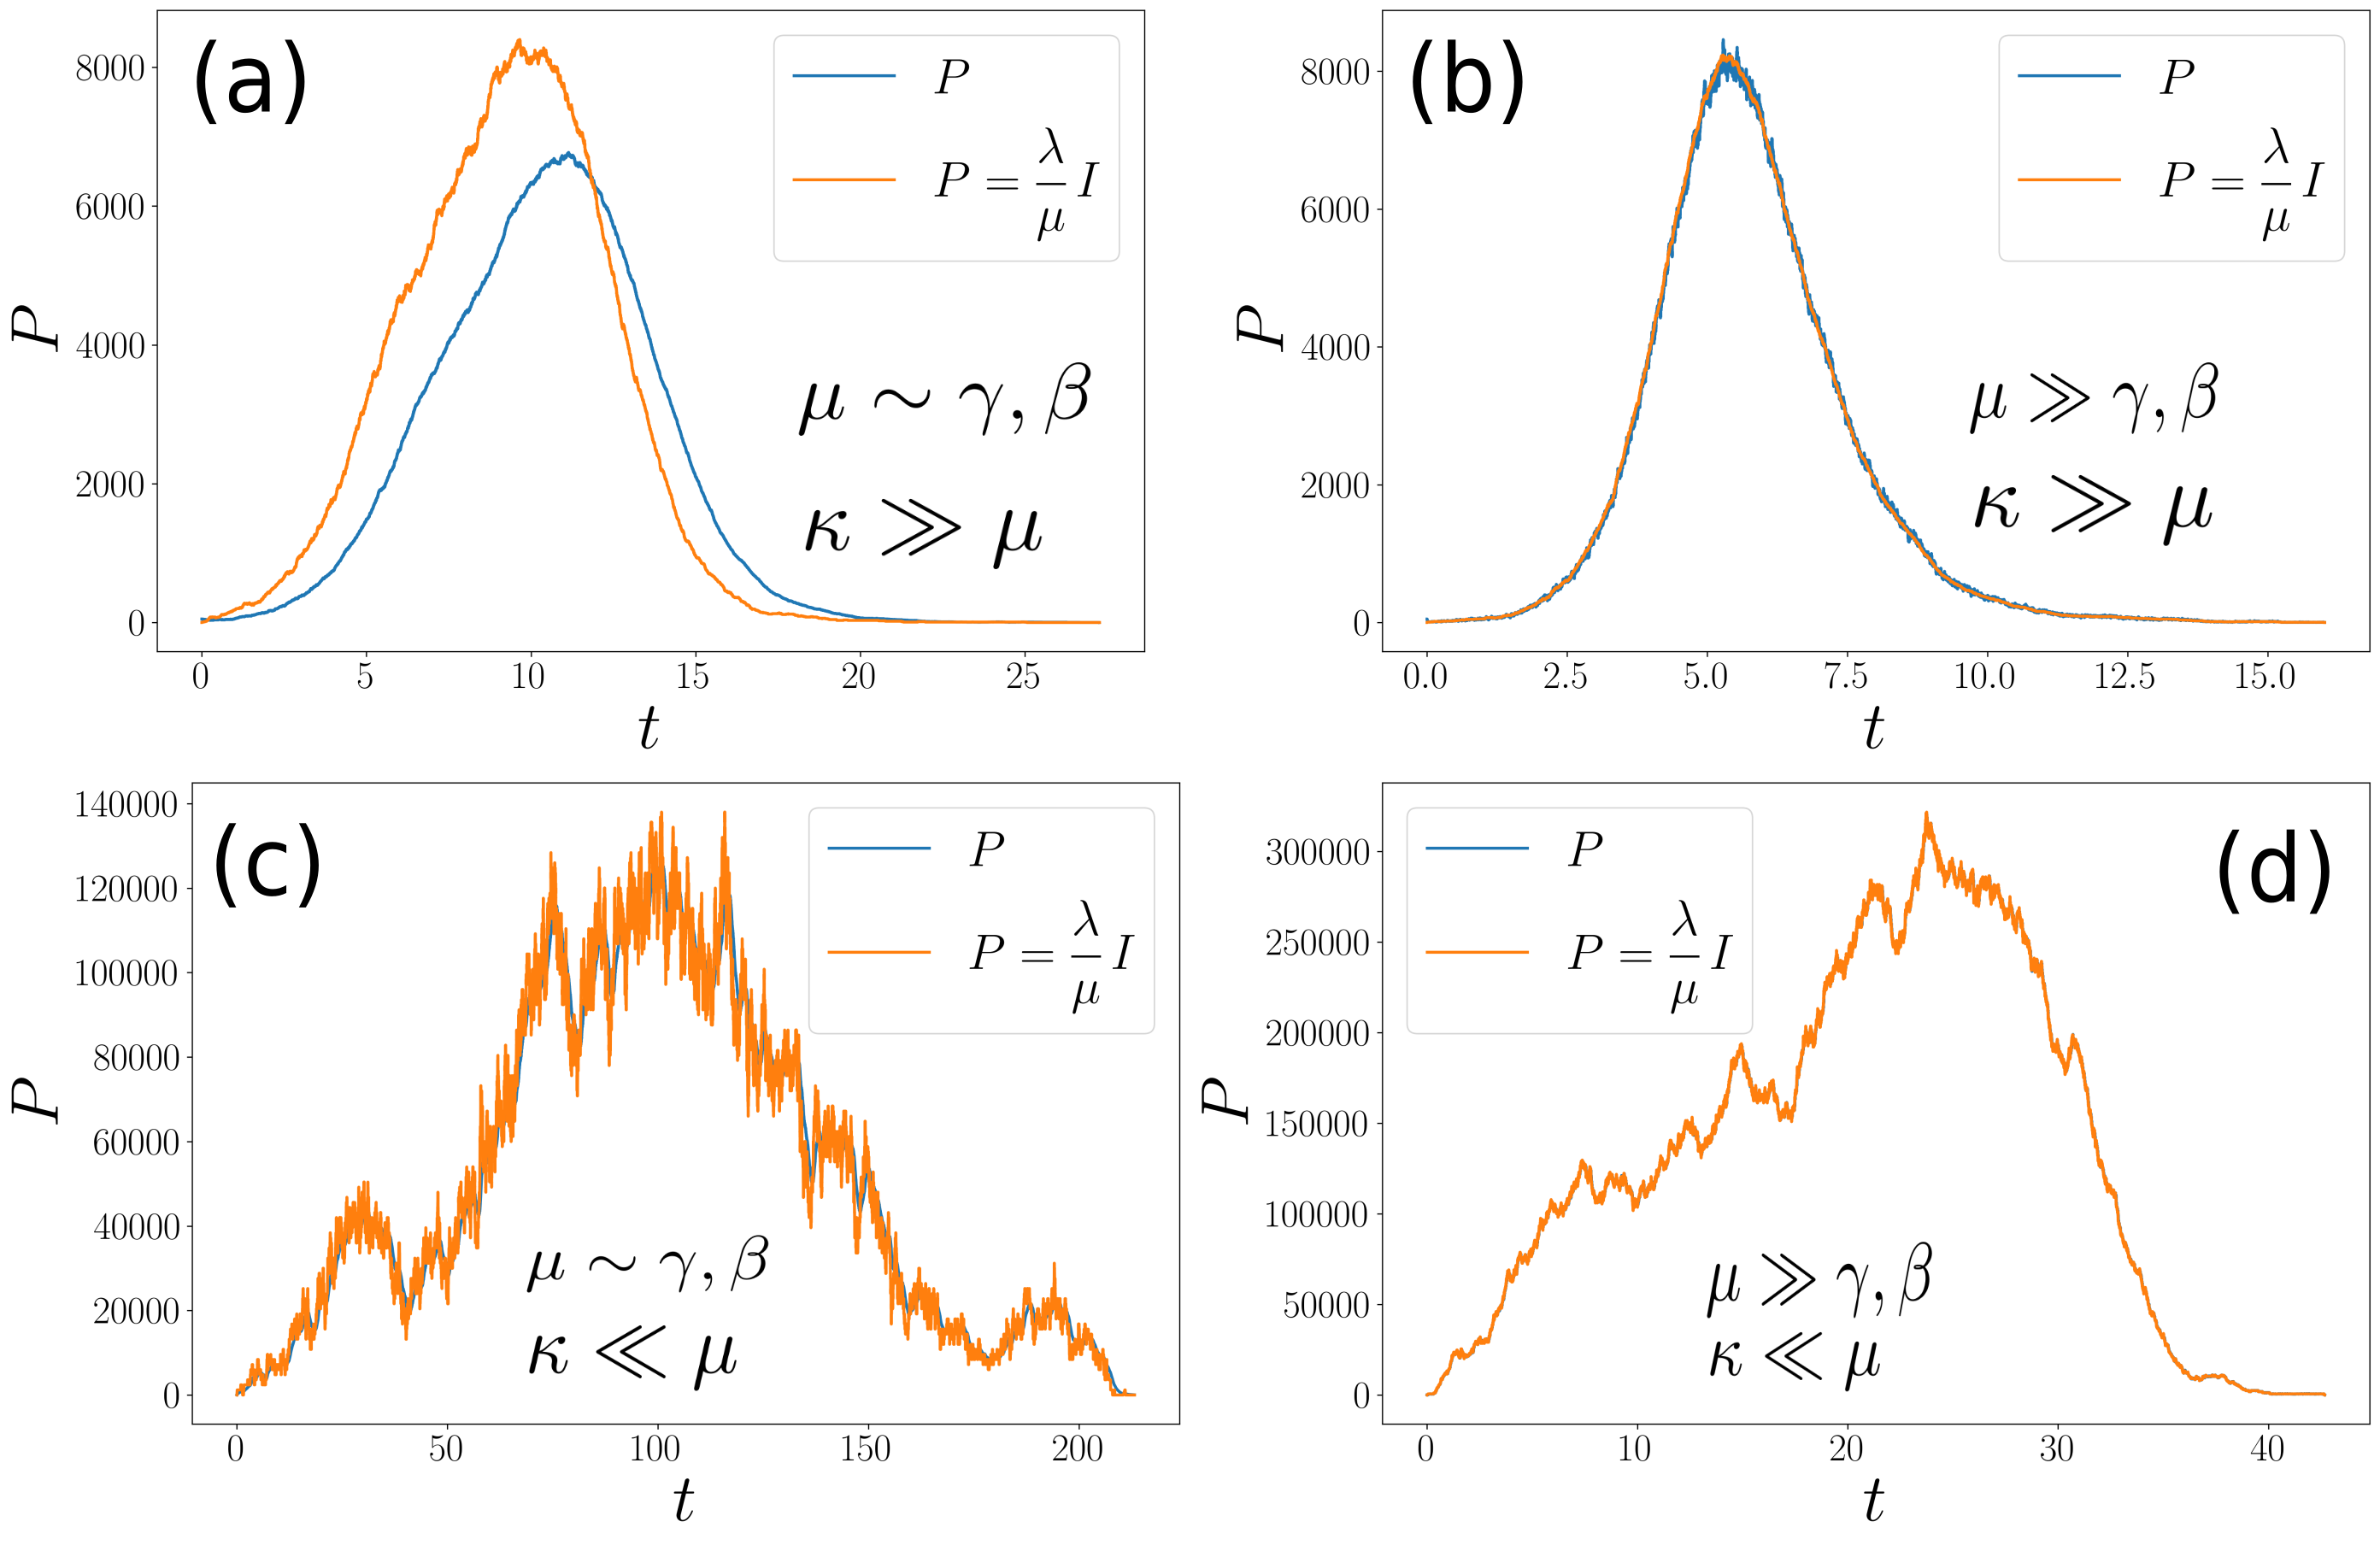
\includegraphics[width=\columnwidth]{Figures/P_approx.png}
    \caption[Validation of the approximate expression for the parasite
        population dynamics]{Numerical verification of the approximate
        expression for the parasite population dynamics, \cref{eq:P_approx_II},
        for different mobility conditions. The simulations were performed
        fixing $\beta=\gamma=1$ for all panels. (a) $\mu=1$ $\kappa=10^2$,
        $\lambda=6.06$, $\kappa/(\mu+\kappa)=0.99$;
        (b) $\mu=100$, $\kappa=10^4$, $\lambda=306$,
        $\kappa/(\mu+\kappa)=0.99$; (c)
        $\mu=1$, $\kappa=0.01$, $\lambda=1200$, $\kappa/(\mu+\kappa)=0.01$; (d)
        $\mu=100$, $\kappa=1$, $\lambda=60600$,  $\kappa/(\mu+\kappa)=0.01$}
    \label{fig:P_approx}
\end{figure}

Thus, for the non-spatial limit ($\kappa\gg\mu$) we have that if
$\mu\gg\beta,\gamma$ \cref{eq:P_approx_II} is valid, while for $\kappa\ll\mu$
the
approximation is also valid regardless of the value of $\beta,\gamma$, as the
nature of the approximation is different. Thus, in general, as $\kappa$
decreases over $\mu$ (the lower the parasite mobility becomes) we expect the
approximation to work better.

The parasite approximation to infected hosts dynamics, \cref{eq:P_approx_II},
is numerically verified for different mobility conditions.
\cref{fig:P_approx}(a)-(b) shows how the approximation improves as $\mu$ grows
over $\beta,\gamma$ (mean errors are $0.18$ and $0.0081$, respectively) in the
non-spatial limit, i.e. $\kappa\gg\mu$, as expected. This result is in perfect
agreement with that found in \cite{GimenezRomero2021}. Then,
\cref{fig:P_approx}(c)-(d) show that the approximation is valid in general when
$\kappa\ll\mu$ but improves anyway when $\mu\gg\beta,\gamma$ (mean errors are
0.04 and 0.0026, respectively). Summarising, we see that the lower the value of
$\kappa$ is with respect to $\mu$ the more valid \cref{eq:P_approx_II} is,
regardless of the value of $\beta,\gamma$, while in the non-spatial limit,
$\kappa\gg\mu$, the condition $\mu\gg\beta,\gamma$ is needed.

\subsection{Spatial threshold}

One of the main questions in epidemiology is to define the conditions under
which an epidemic outbreak occurs, which usually is translated into the
existence of a threshold. In a well mixed (non-spatial) system the basic
reproduction number ($R_0$), that characterises this threshold $R_0=1$, can be
defined exclusively from \textit{intrinsic} parameters of the pathosystem, as
the host-pathogen interaction does not depend on the host spatial structure or
pathogen mobility (see \cref{eq:R0_MF}). In stochastic spatial models this
formulation of $R_0$ breaks down. First of all, in stochastic models, even
above the threshold there is a non-zero probability that the disease is unable
to propagate initially, given by
$P_{\textrm{outbreak}}=1-\parentesi{1/R_0}^{I(0)}$ \cite{Brauer2008}.
Furthermore, the discrete nature of the populations also modifies the estimates
of $R_0$ \cite{KEELING200051}. On the other hand, the introduction of space
changes completely the nature of epidemic outbreaks, modifying the
host-pathogen interactions by means of specific host spatial distributions and
pathogen mobility patterns. Even if the basic reproduction number of the
non-spatial model is above the threshold ($R_0>1$), if parasite mobility is not
large enough, the epidemic will stay locally confined. Thus, one expects that
the threshold at which an epidemic outbreak can propagate to the rest of the
system will depend on the balance between the intrinsic pathosystem parameters
in $R_0$ and parasite mobility, defining a spatial basic reproduction number,
$\tilde{R}_0$.

Having in mind the study in \cref{sec:MFlimit}, we expect that in the high
mobility limit the basic reproduction number is defined by the non-spatial
formula, \cref{eq:R0_MF}. On the other hand, the lower the parasite mobility
is, the more difficult will be for a local outbreak to propagate through the
system. Thus, it is natural to think of an spatial basic reproduction number of
the form $\tilde{R}_0=R_0 f(\kappa)$, where $f(\kappa)$ is an increasing
function of the parasite dispersal rate accounting for parasite mobility
fulfilling $\lim_{\kappa\to\infty}f(\kappa)=1$.

Indeed, some authors recently showed that the spatial basic reproduction
number can be defined as the product between the non-spatial value, $R_0$, and
a factor accounting for spatially-dependent interactions, $f(r)$, in the form
$\tilde{R}_0=R_0f(r)$ \cite{Filipe2003,Filipe2004,Gilligan2021}. However, these
expressions are not analytical \cite{Filipe2003,Filipe2004} or are not directly
related to pathogen mobility \cite{Gilligan2021}. Here we propose a simple
expression for the spatial basic reproduction number regulating the spatial
propagation of the epidemic,
\begin{equation}\label{eq:R_0ibm}
    \tilde{R}_0=\frac{\lambda}{\gamma}\frac{\beta}{\mu+\beta}
    \frac{\kappa}{\mu+\kappa}=R_0\frac{\kappa}{\mu+\kappa}
    \ .
\end{equation}

The derivation of \cref{eq:R_0ibm} accounts for the number of secondary
parasites that are able to produce new infections, or equivalently, the number
of secondary infections produced by an initial infected host. If we consider an
initial infected individual, on average it will produce $\lambda/\gamma$
parasites. Then, these parasites can only move to neighbouring sites or die, so
that the dispersal probability is given by $\kappa/(\mu+\kappa)$. Finally,
considering that parasites do not affect each other trying to infect the same
host, the infection probability is given by $\beta/(\mu+\beta)$. Joining all
terms, we finally obtain \cref{eq:R_0ibm}. This expression is valid when
parasites move only to sites with susceptible individuals and do not try to
infect the same host. Thus, the derived $\tilde{R}_0$ is only an approximation
to the spatial basic reproduction number for the case of an initial
introduction of a small quantity of parasites in a fully susceptible
population.

Note that, as expected, the spatial basic reproduction number is nothing
other than the basic reproduction number of the non-spatial model multiplied by
an increasing function of the parasite mobility, $\kappa/(\mu+\kappa).$ Taking
the limit $\kappa\gg\mu$ in \cref{eq:R_0ibm} (non-spatial limit) the basic
reproduction number of the non-spatial model is recovered. Conversely, in the
limit of very low mobility, the $\kappa/(\mu+\kappa)$ factor is small, and this
has to be compensated with a large value of the non-spatial basic reproduction
number, $R_0$, in order that there is an outbreak, i.e., $\tilde{R}_0>1$.

The spatial threshold, $\tilde{R_0}=1$, given by \cref{eq:R_0ibm}, has been
numerically checked by computing the phase diagram between the absorbing phase
$R(\infty)\approx 0$ (no infection, i.e. disease-free state)  and the active
phase $R(\infty)> 0$ (in which some level of infection has occurred, i.e.
propagation phase) for several values of the parasite mobility and the basic
reproduction number of the non-spatial model, $R_0$ \cref{eq:R0_MF}. The
transition is expected to occur at $\tilde{R}_0=1$, implying from
\cref{eq:R_0ibm} that the dependence of the critical value of $R_0$, say
$R_0^c$, is expected to take the form,
\begin{equation}\label{eq: R_0_crit dependence}
    R_0^c\sim\parentesi{\frac{\kappa}{\mu+\kappa}}^{-1} \ .
\end{equation}
As discussed above, we expect that $\tilde{R}_0=1$ with $\tilde{R}_0$ given
by \cref{eq:R_0ibm} does not represent exactly the spatial threshold, and for
this reason we suggest the more general functional form,
\begin{equation}\label{eq: threshold_corrections}
    R_0^c\sim A\parentesi{\frac{\kappa}{\mu+\kappa}}^{-B} - C\ ,
\end{equation}
to be be fitted to numerical data, where $A=1$, $B=1$ and $C=0$ would imply
a perfect agreement of numerical simulations of the IBM model with
\cref{eq:R_0ibm}.

In order to obtain the phase diagram, we compute the absorbing state of the
model as an average over $1000$ realisations for each value of the mobility and
$R_0$ considered. Then, the critical value $R_0^c$ is computed for each
mobility value as the $R_0$ value for which the fluctuations of the ``order
parameter'' $\displaystyle \chi=\avg{{R(\infty})^2}-\avg{R(\infty)}^2$ are
maximal, as this would be an indication of a transition between the
disease-free and the propagation phases.

\begin{figure}[H]
    \centering
    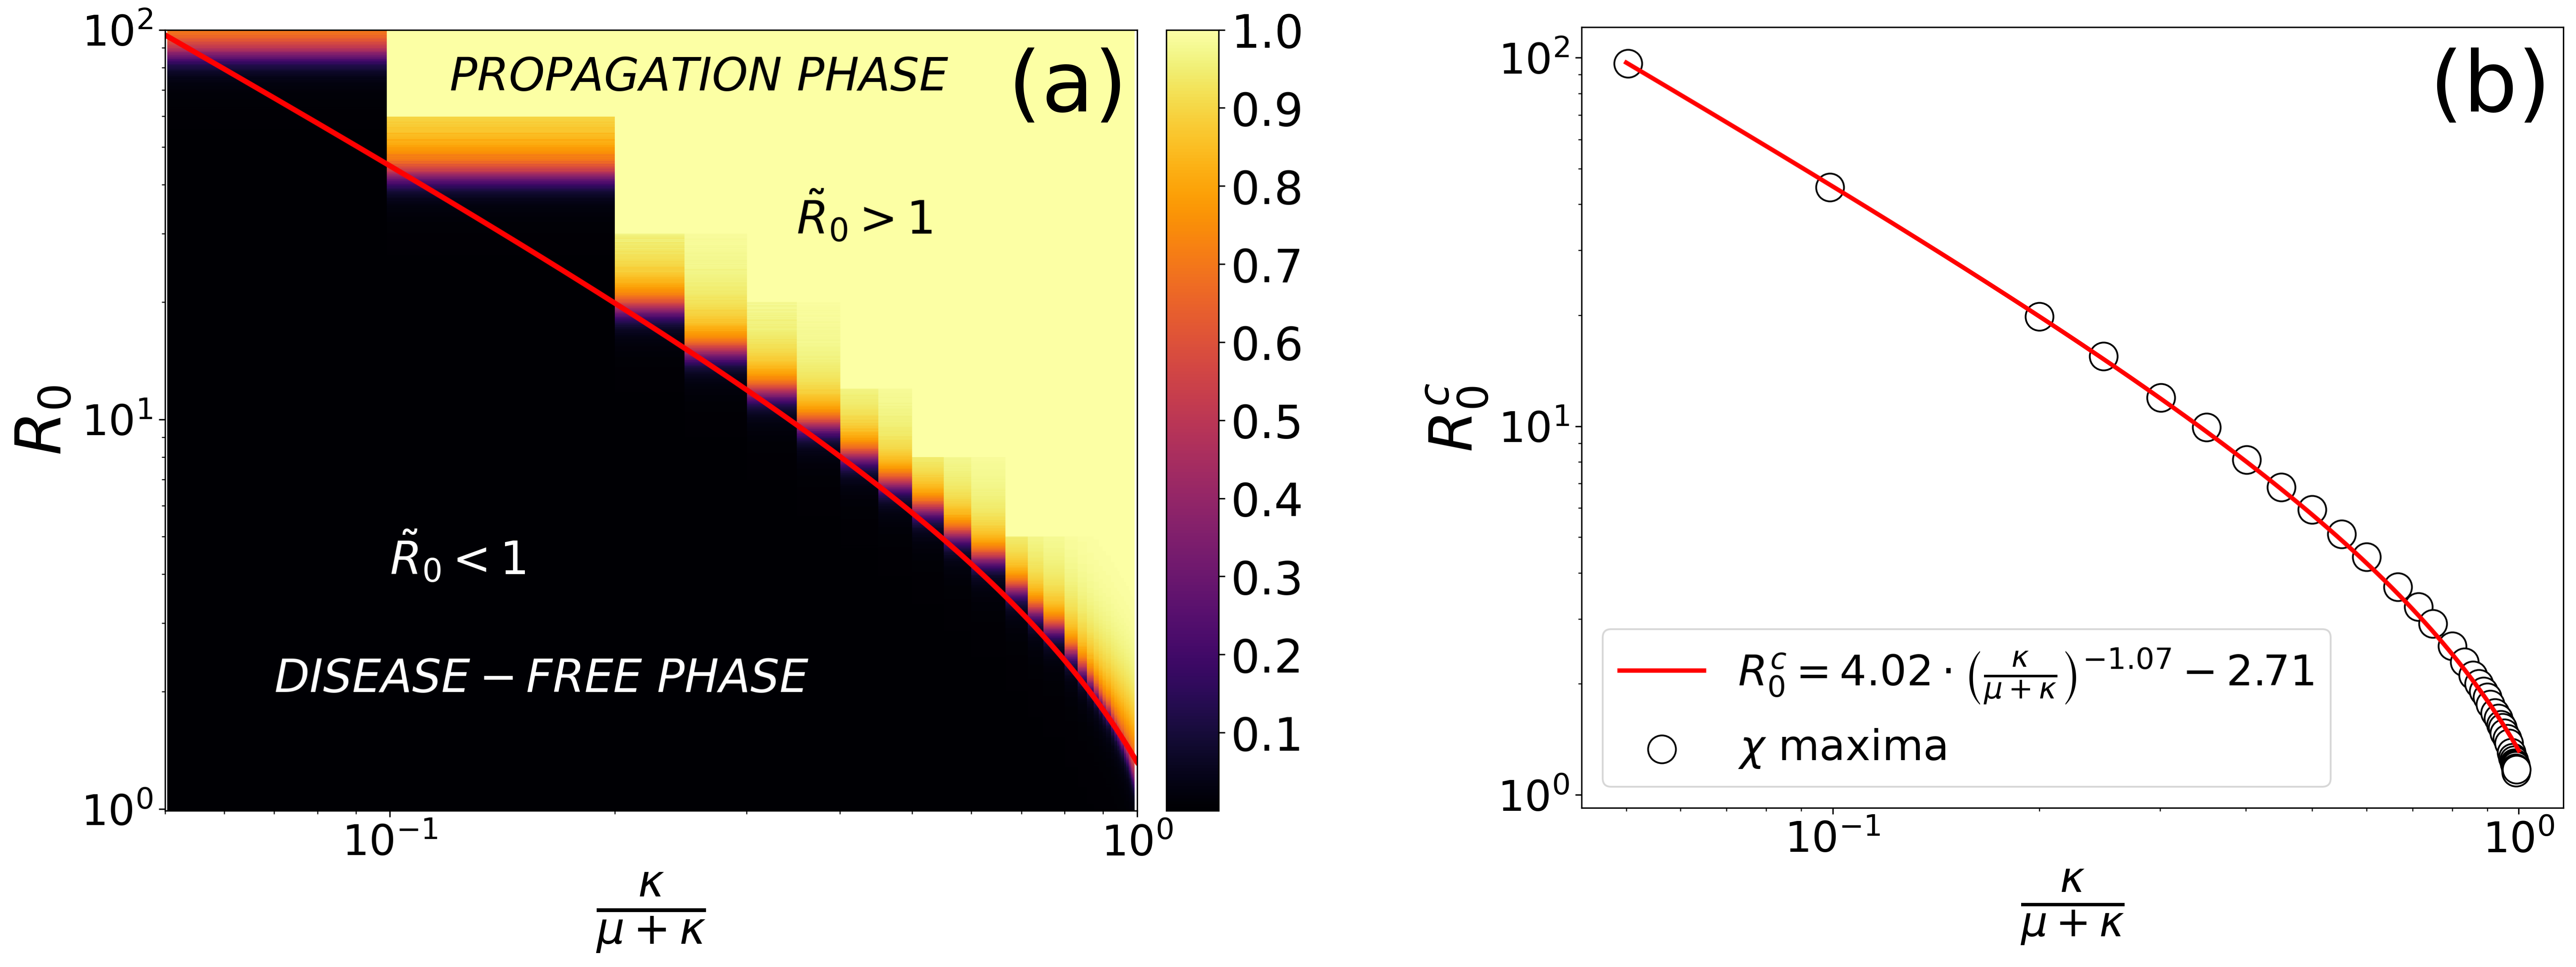
\includegraphics[width=1\textwidth]{Figures/PhaseDiagram.png}
    \caption[
        Phase diagram and fit for the transition between the disease-free and
        propagation phases]{(a) Phase diagram showing the transition between
        the the
        disease-free phase and the propagation phase for several values of the
        parasite
        mobility and $R_0$. The colour code represents the fraction of dead
        individuals
        (i.e. $R/N$) in the final state of the epidemic computed by the average
        over
        1000 realisations. (b) Fit for the transition line following \cref{eq:
            threshold_corrections}, where dots are the maximums of the ``order
        parameter''
        fluctuations, $\chi=\avg{{R(\infty})^2}-\avg{R(\infty)}^2$}
    \label{fig:Phase_diagram}
\end{figure}

\cref{fig:Phase_diagram}(a) shows the numerical results of the computed
transition between the disease-free and propagation phases. The heatmap coding
represents the average value of absorbing state $\avg{R(\infty)}$ for several
values of the mobility factor and $R_0$. As expected, the lower the mobility
factor is, the higher the value of $R_0$ is needed for the disease to invade
the population. \cref{fig:Phase_diagram}(b) shows the fit of \cref{eq:
    threshold_corrections} with less than a $1\%$ of relative error.
Interestingly,
we obtain $B=1.07\approx1$ which validates our expression for the spatial
threshold as a first approximation. However, the values for $A=4.02$ and
$C=2.7$ show a significant deviation from \cref{eq: R_0_crit dependence} and
indicate that the expression \cref{eq:R_0ibm} is  an approximation to the
spatial basic reproduction number, which however seems to contain the right
dependence on $\kappa/(\mu+\kappa)$, and where $A$ could be a geometric factor
for a lattice.

\subsection{Spreading speed of the infected population and time to extinction}

Another relevant epidemiological question is how does an infected
population spread after the onset of an epidemic. In order to obtain this
spreading speed we computed the mean time needed for an infected individual to
reach the boundary of the system. More specifically, for each particular choice
of the model parameters, 1000 simulations were run for several system sizes
ranging from $L=10$ to $L=60$. The computed mean time was found to depend
linearly with the system size, thus allowing to compute the speed from the
slope of this relation. With this procedure, the spreading speed was computed
for several values of the parasite mobility and $R_0$, large enough to ensure
an epidemic outbreak that reached the boundary of the system. In this
situation, the spreading speed is expected to depend linearly with the square
root of the parasite mobility,
\begin{equation}\label{eq:front_vel}
    v\sim\sqrt{\kappa} \ .
\end{equation}

\cref{fig:front_velocity}(a) shows this square root dependence for
different values of the fixed $R_0$. Similarly, the speed was also computed for
several values of the basic reproduction number and a fixed mobility. In this
case, it varies with the square root of the distance to the critical value of
$R_0$, $R_0^c$, as shown by \cref{fig:front_velocity}(b). This is in good
agreement with other mathematically similar models \cite{Bertuzzo2010}.

\begin{figure}[H]
    \centering
    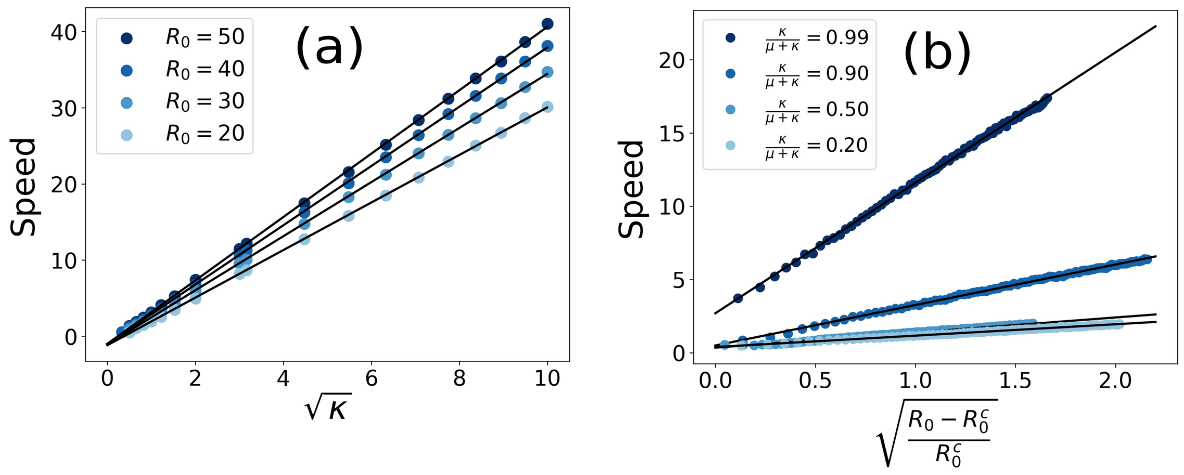
\includegraphics[width=1\textwidth]{Figures/Front_velocity.png}
    \caption[
        Analysis of the spreading speed of the infected population
    ]{(a) Disease spreading speed as function of the square root of
        the parasite mobility for several values of $R_0$. The plot shows a
        remarkable
        agreement with \cref{eq:front_vel}. (b) Disease spreading speed as
        function of
        the square root of the distance to the critical value of $R_0$ for
        several
        values of the parasite mobility.}
    \label{fig:front_velocity}
\end{figure}

The extinction time is defined as the time elapsed from the beginning of
the epidemic until the system reaches its absorbing state, that is, when no
parasites or infected individuals are left. From \cref{eq:front_vel}, we expect
the time to extinction to increase when the parasite mobility is decreased.
Moreover, we expect the extinction time to decrease with the distance to the
epidemic threshold, as we expect to reach faster the absorbing state for larger
values of the spatial basic reproduction number.

In the limiting case where all (or almost all) hosts die, it is clear that
the disease must have spread to the entire system. Thus, in this limit, the
extinction time should be proportional to the inverse of the disease spreading
speed, $t_{\textrm{ext}}\sim 1/v$. Then, in this limit, we can relate the
extinction time with the parasite mobility as follows,
\begin{equation}\label{eq:t_ext}
    t_{\textrm{ext}}\sim\frac{1}{\sqrt{\kappa}} \quad \textrm{for} \quad
    \tilde{R}_0\gg1 \ .
\end{equation}
However, the absorbing state is not always reached after all hosts becoming
infected and \cref{eq:t_ext} is only expected to work far from the epidemic
threshold, when the disease is expected to spread to the entire system.

In \cref{fig:extinction_time}(a) the extinction time is plotted against the
basic reproduction number for some values of the parasite mobility. As
expected, the extinction time increases for lower values of the parasite
mobility. The increasing behaviour before the peak can be understood as the
increasing time needed for the initial perturbations to decay to the
disease-free phase. After the peak, the greater the basic reproduction number
the faster the epidemic will reach its absorbing state with a non-negligible
number of dead individuals. So, with this interpretation, the peaks of the
extinction time should coincide with the epidemic threshold for each value of
the parasite mobility.

\begin{figure}[H]
    \centering
    \includegraphics[width=\textwidth]{Figures/Extinction_time.png}
    \caption[
        Analysis of the extinction time of the epidemic]{(a) Extinction time
        for some values of the parasite mobility.
        (b) Comparison of the critical $R_0$ value computed with
        \cref{eq:R_0ibm}
        compared to the values obtained numerically by computing the maximum of
        the
        extinction time. (c) Scaling of the extinction time with several values
        of the
        parasite mobility. (d) Representation of the square of the extinction
        time as
        function of the inverse of the parasite mobility. The inset shows the
        zone
        where this relation has been computed, showing a good agreement with
        \cref{eq:t_ext}.}
    \label{fig:extinction_time}
\end{figure}

In \cref{fig:extinction_time}(b) we compare the numerical value of $R_0$ at
which the extinction time peaks with the theoretical value of $R_0^c$, computed
with \cref{eq: threshold_corrections}, showing good agreement. Thus, the
dependence of the extinction time with $R_0$ should vanish if plotted against
the distance to $R_0^c$. Furthermore, if the extinction time is normalised
(dividing each line by its maximum), all the lines should collapse near the
transition point. In \cref{fig:extinction_time}(c) the normalised extinction
time is plotted against the distance to the critical value of $R_0$. The
scaling is shown to be valid only near the transition point, as expected.

In the limiting case where the epidemic dies by infecting a large part of
the host population, i.e. for a large enough $R_0$ value, the extinction time
should follow \cref{eq:t_ext}, as previously discussed. In
\cref{fig:extinction_time}(d) we show how the extinction time relates to the
parasite mobility in this limit, following the predicted behaviour.

\section{Conclusions} \label{sec: conclusions}

In this work we have developed a spatially-explicit individual-based model
for parasite-produced marine epidemics of immobile hosts. This study has
allowed us to tackle important questions in marine epidemiology, as how spatial
constraints affect epidemic spreading in filter-feeder populations or how will
the infected population of hosts change in space and time. While addressing the
aforementioned questions, we have shown that there exists a regime of high
parasite mobility where the time progression of both host and parasite
populations can be well described by the non-spatial version of the model (i.e.
the system of ODE's presented in \cite{GimenezRomero2021}). We have also shown
that a fast-slow approximation for the time progression of the parasite
population, already presented in \cite{GimenezRomero2021}, can be extended for
spatial systems. Interestingly, the conditions under which this approximation
is valid  are less restrictive than in the non-spatial case, and regimes in
which this approximation is valid for low mobility and comparable time scales
are reported in this contribution.

We have derived an approximate analytical expression of the
\textit{spatial} basic reproduction number, that allows to predict the onset of
a global epidemic in a spatial model. The obtained expression explicitly shows
a trade-off between the intrinsic pathosystem dynamics (i.e. $R_0$) and a
factor accounting for parasite mobility. Moreover, the spatial threshold
defined by $\tilde{R}_0=1$ separates the final state of the system in two
different phases, namely a disease-free phase and a propagation phase. In the
propagation phase, any initial condition of infected individuals or parasites
will propagate throughout the system, causing a proper outbreak. On the other
hand, in the disease-free phase the conditions are not sufficient for a local
introduction of parasites or infected individuals to spread through the system.
The effect of the parasite mobility in the spatial basic reproduction number is
clear, the more parasites move the more infections they cause.

The spatiotemporal behaviour of the system has been investigated in the
propagation phase. First, we showed that the infected population spreads
through the space with a speed directly proportional to the square root of the
diffusion coefficient of parasites, showing good agreement between the derived
analytical expression and numerical simulations. The time to extinction has
been also studied by means of numerical simulations, showing that, if the
system is far above enough of the spatial threshold, the time to extinction can
be analytically computed, in good agreement with simulations. We obtained that
larger values of the parasite mobility yield more severe epidemics in which
there are more infections and the extinction is faster.

To summarise, in the present work we have introduced and analysed and
Individual-Based approach to epidemic transmission in spatially extended
systems of immobile hosts. The infection mechanism is due to mobile parasites,
that are in turn produced by infected hosts. The study allows to answer some
biologically relevant questions, like predicting the occurrence of a global
epidemic outbreak or its velocity of expansion through the system. Thus, the
analytical and computational results of the model shed light on the underlying
mechanisms underpinning the emergence of a global epidemic outbreak and its
spatial progression. This work provides a first step into the spatial-explicit
individual-based modelling of marine epidemics of immobile hosts.

Although this work has considered the case of a spatially homogeneous
distribution of hosts, we plan to extend the study to more general cases,
discussing the effect of inhomogeneous spatial host distributions. Furthermore,
other biological relevant effects could be added to the model to enhance the
description of different epidemics, e.g. infected individuals could still
filter parasites or parasite-load dependent infection process. The model could
also describe epidemics on other immobile species such as filter feeders like
sponges or other bivalves, corals, intertidal communities or starfishes
provided that the necessary modifications in the model are properly included.
Stochastic spatially-explicit descriptions like the one presented here could be
also extended to the study of epidemics of other immobile hosts, like
vector-borne diseases of plants. However, this would imply a quite different
model to describe the different epidemic compartments of the vectors and also
their ecological features. We hope these studies can be useful in conservation
plans or ecosystem management and could serve as a basis for more sophisticated
models.

%----------------------------------------------------------------------------------------
%	PART III: Towards more realistic models for Xylella fastidiosa spread
%----------------------------------------------------------------------------------------

\part{Realistic models for vector-borne plant diseases}

%----------------------------------------------------------------------------------------
%	Vector-borne diseases with non-stationary vector populations: the case
%   of growing and decaying populations
%----------------------------------------------------------------------------------------
\chapterimage{olivar_tramuntana.jpg}
\chapterspaceabove{6.75cm}
\chapterspacebelow{7.25cm}

\chapter{Vector-borne diseases with non-stationary vector populations: the case
  of growing and decaying populations}
\vspace{1cm}

\textbf{Àlex Giménez-Romero$^{1}$, Rosa Flaquer-Galmés$^{1,2}$, Manuel A.
    Matías$^{1}$}

\vspace{1cm}

\begin{enumerate}
    \small
    \item Instituto de Física Interdisciplinar y Sistemas Complejos, IFISC
          (CSIC-UIB), Palma de Mallorca 07122, Spain
    \item Grup de Física Estadística, Departament de Física. Facultat de
          Ciències, Universitat Autònoma de Barcelona, 08193 Bellaterra
          (Barcelona),
          Spain

\end{enumerate}

\vspace{1cm}

\textbf{Published as}

\vspace{0.5cm}

\fullcite{GimenezRomero2022_PRE}

\newpage
\section{Introduction}\label{sec:intro}

Vector-borne diseases are caused by infectious agents transmitted by living
organisms, called vectors,  frequently insects. These diseases represent a
significant threat to global human health \cite{Athni_2020}, causing diseases
such as malaria, dengue, yellow fever, Zika, trypanosomiasis and leishmaniasis
\cite{SCHUMACHER2018352}. Vector-borne human diseases are responsible of more
than 17\% of all human infectious diseases, causing millions of cases and more
than $700\,000$ deaths annually \cite{WHO}. Moreover, crop production and farm
profitability are also affected by bacterial \cite{HUANG20201379} and virus
\cite{Bragard2013} vector-borne diseases. Some examples are the Pierce's
Disease of grapevines, that has resulted in an annual cost of approximately
\$100 million in California alone \cite{tumber2014pierce}, the olive quick
decline syndrome, which could cause about 5 and 17 billion US\$ of losses in
Italy and Spain over the next 50 years in the absence of disease control
measures \cite{Schneider2020} and the multiple diseases caused by viruses
\cite{Rybicki2015}, with diseases like the tobacco mosaic, tomato spotted
wilt, etc., transmitted by aphids and other vectors.

Compartmental deterministic models, e.g. the well known SIR model
\cite{McKendrick}, have been widely used in the modeling of vector-borne
diseases after the seminal work of Ross and Macdonald \cite{Macdonald1957},
that opened the way to controlling malaria outbreaks by acting on the vectors
of the disease (the \textit{Anopheles} mosquito). These models consider that
both host and vector populations can be divided into different compartments
describing different states of the individuals, such as susceptible, infected
or removed (recovered or dead) \cite{Brauer2008}, and the time-evolution of
these compartments is expressed as a system of ordinary differential equations,
defining a dynamical system. Compartmental models provide a mean-field
description, that imply well-mixed (in practice spatially homogeneous)
populations. The well mixed approximation will be valid whenever the mean
distance among hosts is smaller than the mixing length of vectors before they
die. In the case of vector-borne diseases it is also equivalent to every vector
effectively interacting with all the hosts and every host with all the vectors.
A mean-field description is not always valid in spatially extended systems, but
still it is often the first step before writing a spatially explicit
description.

The most relevant piece of information about a disease is whether an
epidemic outbreak will take place or not. The \textit{basic reproduction
    number}, $R_0$, measures the number of secondary infections caused by an
initial infected individual in a fully susceptible population, defining the
epidemic threshold \cite{Anderson1991, VandenDriessche2017}, that determines
the emergence (or not) of an outbreak. If $R_0>1$ an epidemic outbreak will
occur, while there will be no outbreak otherwise. The standard way of computing
$R_0$ in deterministic compartmental models is based on the existence of an
initial disease-free (pre-pandemic) equilibrium, represented by the absence of
infected hosts and vectors \cite{Lauko2006, Kamgang2008}. Some standard
methods based on the linear stability condition of this equilibrium have been
developed to allow the direct computation of $R_0$, such as the Next-Generation
Matrix (NGM) method \cite{Diekmann2010}.

In the case of vector-borne diseases, some models assume that populations
(both hosts and vectors) do not change with time (see e.g.
\cite{Macdonald1957, Brauer2016, VandenBosch2017}), thus assuming equal birth
and death rates. This guarantees the existence of a disease-free equilibrium
and the proper use of standard methods to determine $R_0$. However, this
assumption could be far from reality in several pathosystems. For example, the
interaction between temperature, precipitation variations and other factors may
lead to strong variations in the vector population
\cite{garms1979studies,Rocklov2020}, implying that the pre-pandemic state may
not be an equilibrium state and that standard methods cannot be applied.

Compartmental models of vector-borne diseases have another feature that may
hinder their practical applicability. Namely the fact that these models have
many compartments, that describe the different states of both hosts and
vectors, and as a consequence a relatively large number of parameters. This may
lead to an issue known as \textit{parameter identifiability and uncertainty}
\cite{Chowel2017}, depending on the available data, that is more likely to be
found in models with many compartments and parameters \cite{Roosa2019}.
Usually, parameter estimation procedures are needed to connect the models with
disease data, mainly using incidence or prevalence over time in the host
population. Unfortunately, under many circumstances the underlying model
parameters are unidentifiable, so that many different sets of parameter values
produce the same model fit \cite{Kao2018}. Moreover, these parameters can be
really difficult to determine from the available experimental data.
Nevertheless, in some cases, mathematical manipulations can be performed to
reduce the model complexity using exact or approximate relations
\cite{GimenezRomero2021}. In such cases, the number of parameters of the models
can
be usually reduced in terms of new parameters defined as combinations of some
of the original parameters.

The plan of this paper is as follows. In \cref{sec:model} we develop a
compartmental model of vector-borne transmitted diseases with constant, but
different, birth and death rates for the vectors, that we will use to describe
the case of growing and decaying vector populations. For simplicity, the model
assumes that there is no host to host direct transmission and that the
development of the disease is faster than host recruitment, which is also a
realistic assumption in  many cases, like plant diseases. \cref{sec:results}
contains the main results of the study. In particular, we show that the
asymptotic approach fails to estimate the $R_0$ of the model, overlooking
outbreaks if some conditions are fulfilled. Here, we provide an alternative
method to compute $R_0$ based on the average number of secondary host
infections produced by a primary infected host in one generation. It turns out
that the validity of the  asymptotic approach depends, among other things, on
some time-scales of the model. Furthermore, we discuss and apply some
approximations that allow to reduce the model in favor of simpler ones, with
both fewer compartments and fewer parameters. In particular, we show that if
some of the parameters fulfill certain conditions, it is possible to reduce the
original model with five compartments and four parameters to a SIR model, with
three compartments and two parameters. It is expected that model reductions
like this one significantly help in solving possible problems of parameter
unidentifiability that plague these models. It is interesting to note that a
model in which hosts do not interact directly, but only through vectors, in a
certain limit becomes described as if hosts would infect directly one to each
other, what is assumed in some studies without suitable confirmation. Finally,
the main concluding remarks of the study are presented in
\cref{sec:conclusions}.

\section{The model}\label{sec:model}

The compartment model for vector-borne diseases that we will use to
illustrate the points to be discussed in this study consists of $5$
compartments, $3$ of which describe the host population (susceptible, $S_H$,
infected, $I_H$, and removed, $R_H$), while the other $2$ describe the vector
population (susceptible $S_V$ and infected vectors, $I_V$). Thus, we consider
that the pathogen affects only the hosts and do not consider exposed
compartments. In addition, no direct host to host or vertical (or mother to
offspring for vectors) transmission is assumed. The model could be also
generalized to include an exposed host compartment and the above mentioned
transmission modes, which would hinder the theoretical analysis without
altering the qualitative conclusions of the study. Finally, for the host
population we consider neither recruitment nor natural death and then the total
host population, $N_H$, is constant, $N_H=S_H+I_H+R_H$. Finally, we assume that
infected hosts do not have a mechanisms to combat the disease and become
susceptible again. These assumptions are reasonable in the case of many
phytopathologies.

The model is defined according to the following processes,
\begin{equation}\label{eq:scheme_infection}
    \begin{aligned}
         & S_H+I_V \stackrel{\beta}{\rightarrow} I_H + I_V \quad I_H
        \stackrel{\gamma}{\rightarrow} R_H                           \\
         & S_V+I_H \stackrel{\alpha}{\rightarrow} I_V+I_H \quad S_V
        \stackrel{\mu}{\rightarrow} \varnothing \quad I_V
        \stackrel{\mu}{\rightarrow}
        \varnothing
        \ ,
    \end{aligned}
\end{equation}
which are graphically described in \cref{fig:model_diagram}, being the
birth of new susceptible vectors described as a source term.
Thus, the host-vector compartmental model is written as,
\begin{equation}\label{eq:SIR_v}
    \begin{aligned}
        \dot{S}_H & =-\beta S_H I_v / N_H                     \\
        \dot{I}_H & =\beta S_H I_v / N_H - \gamma I_H         \\
        \dot{R}_H & =\gamma I_H                               \\
        \dot{S}_v & = \delta C-\alpha S_v I_H / N_H - \mu S_v \\
        \dot{I}_v & =\alpha S_v I_H / N_H - \mu I_v \ ,
    \end{aligned}
\end{equation}
where the crossed nonlinear terms, $S_x I_y$ are written divided by the
total host population, $N_H$, what corresponds to the so called standard
incidence, which differs of the purely bilinear form known as mass action
incidence \cite{MartchevaBook}.

The model describes infection of susceptible hosts, $S_H$, at a rate
$\beta$ through their interaction with infected vectors, $I_v$, while
susceptible vectors, $S_v$, are infected at a rate $\alpha$ through their
interaction with infected hosts $I_H$. Infected hosts exit the infected
compartment at rate $\gamma$, while infected vectors stay infected the rest of
their lifetime, as we consider that the pathogen does not affect them, as it is
customary. Vectors die naturally (or disappear from the population by some
mechanism) at rate $\mu$ and are born (appear) at a constant rate $\delta$
being susceptible. The constant term $C$ sets the scale of the stationary value
of the vector population. \cref{fig:model_diagram} shows an schematic
representation of the model and we refer to \cite{Brauer2016} for a similar
model of vector-borne diseases. However, the model in \cite{Brauer2016}
includes exposed compartments and direct host to host transmission, but assumes
that the birth and death rate of vectors are identical, and thus, the
population does not change with time and stays as fixed by the initial
condition.
\begin{figure}[H]
    \centering
    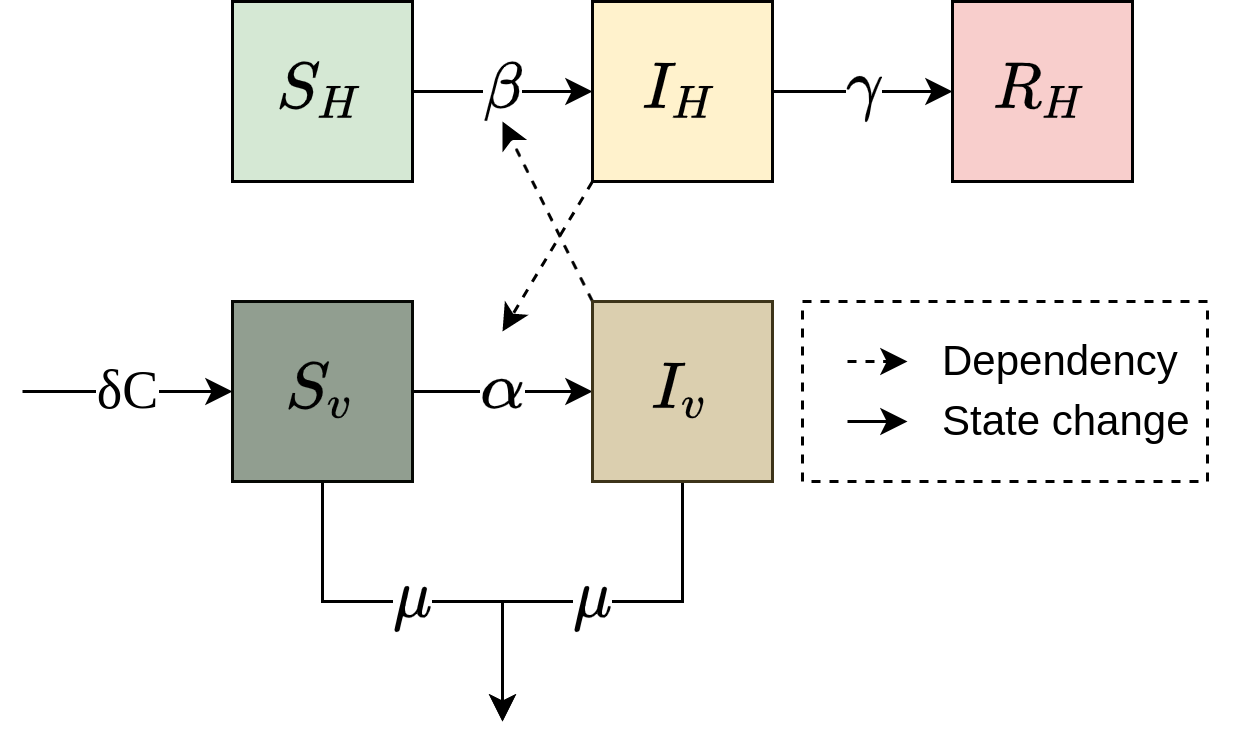
\includegraphics[width=0.9\textwidth]{Figures/Diagram.png}
    \caption{Schematic representation of the model n \cref{eq:SIR_v}. Boxes
        are the compartments in which the population is divided, solid arrows
        represent
        changes in state (so transitions between compartments), and dashed
        arrows
        depict the crossed interaction between hosts and vectors.}
    \label{fig:model_diagram}
\end{figure}

\subsection{Preliminary analysis of the model} \label{sec:Prelimanalysis}

From \cref{eq:SIR_v} it is straightforward to verify that the population of
hosts remains constant over time, $N_H=S_H+I_H+R_H$, while the vector
population fulfills,
\begin{equation}\label{eq:dif_eq_Nv}
    \dot{N}_v=\dot{S}_v+\dot{I}_v=-\mu\parentesi{S_v+I_v}+\delta C=-\mu N_v
    + \delta C \ ,
\end{equation}
with solution,
\begin{equation}\label{eq:Nv_t}
    N_v(t)=\frac{\delta}{\mu}C +
    \parentesi{N_v(0)-\frac{\delta}{\mu}C}e^{-\mu t} \ .
\end{equation}
From \cref{eq:Nv_t} one can write the stationary value for the vector
population, $N_v^*$,
\begin{equation}
    N_v^*=\lim_{t\to\infty}N_v(t)=\frac{\delta}{\mu}C \ .
    \label{eq:asympt}
\end{equation}
Thus, if the initial population of vectors is below (above) the stationary
value, the vector population will grow (decrease) until it reaches the
stationary value. On the other hand, if $N_v(0)=N_v^*=\delta C/\mu$ the initial
population of vectors is already at the stationary state. The initial condition
for the vector population can be written in terms of its stationary value
\cref{eq:asympt}, $N_v(0)=fN_v^*$, where both $f<1$ and $f>1$ are possible, so
that one gets,
\begin{equation}\label{eq:Nv_t_fraction}
    N_v(t)=N_v^*\claudator{1+\parentesi{f-1}e^{-\mu t})} \ .
\end{equation}

We note that vector-borne disease models that assume constant vector
populations (e.g.\cite{Brauer2016}) can be recovered by setting $\delta=\mu$
and $C=N_v(0)$, so that any initial condition for the vector population is
stationary, i.e. $\dot{N}_v=0$ in \cref{eq:dif_eq_Nv} and $N_v(t)=N_v(0)$. We
note that our model describes populations with an asymptotic stationary vector
population and cannot describe periodic vector populations.

\section{Results} \label{sec:results}

%\subsection{The basic reproduction number for stationary vector populations}
\subsection{Epidemic threshold and disease dynamics}
\label{sec:R0statvp}

\begin{figure*}[t!]
    \centering
    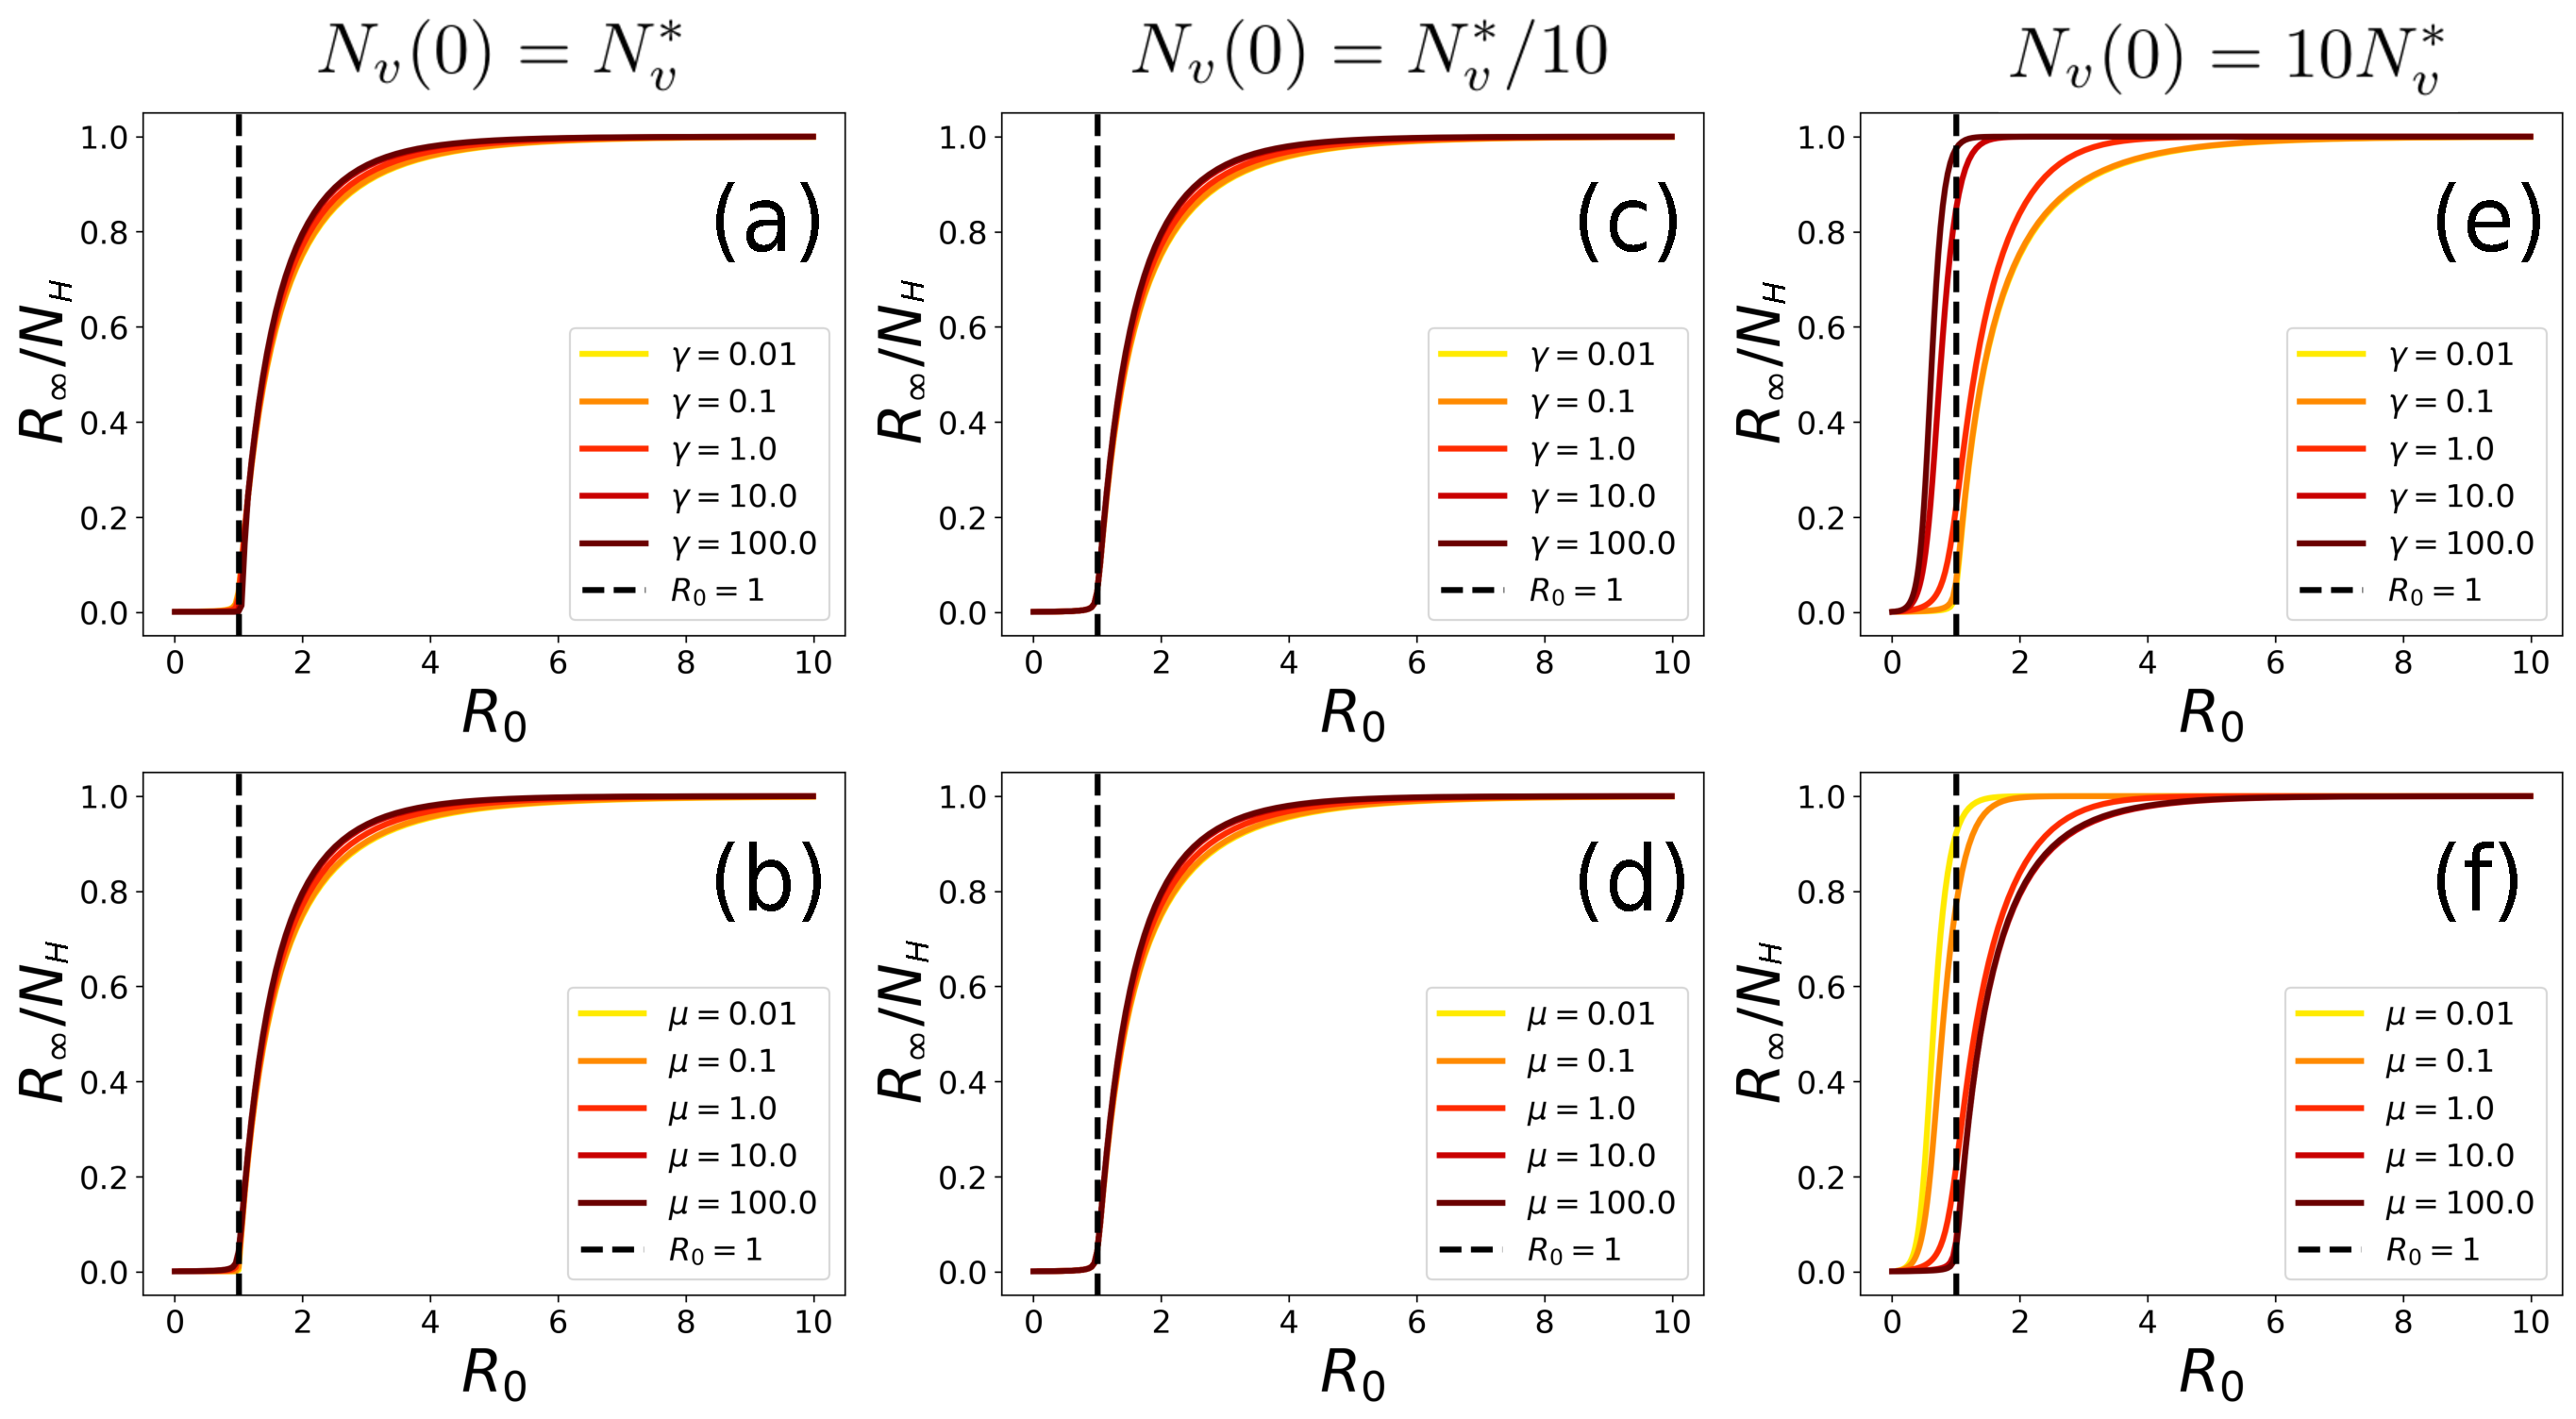
\includegraphics[width=\textwidth]{Figures/R0_check_stationary.pdf}
    \caption{Numerical verification of the predictive  power of the basic
        reproduction number relation \cref{eq:R0_asympt}, by plotting the final
        size of
        the epidemic, $R_\infty/N_H$ as function of $R_0$. In panels (a),(b)
        the
        initial vector population is in the stationary value, in panels (c),(d)
        is
        below, $N_V^*/10$, and in panels (e),(f) above, $10 N_V^*$. Panels
        (a),(c),(e)
        show realisations for different $\gamma$ values with a fixed $\mu=1$
        baseline
        value. Panels (b),(d),(f) show realisations for different $\mu$ values
        with a
        fixed $\gamma=1$ baseline value.}
    \label{fig:R0_check_stationary}
\end{figure*}

Let us start with the cases in which any initial condition for the vector
population is stationary  and the total vector population remains unchanged.
This will happen when the birth $\delta$ and death $\mu$ vector rates are
identical, independently on the initial condition of the vector population, or
the case in which the initial condition of the vector population is already at
its stationary value, $N_v(0)=N_v^*$, independently of the values of $\delta$
and $\mu$. In such a case, the initial disease free state of the model, given
by $I_H(0)=I_v(0)=0$, is a fixed point (equilibrium state) of the dynamical
system \cref{eq:SIR_v} independently of the other initial conditions for the
host and vector populations. This allows the definition of the basic
reproduction number, $R_0$, using standard methods such as linear stability
analysis or the Next-Generation Matrix (NGM) method \cite{Diekmann2010} (see
\cref{app:R0_standar_methods}).

In other cases, the total vector population will vary with time provided
that the initial condition, $N_v(0)$, is not identical to the asymptotic value
at large times, $N_v^*$. In these cases, an initial disease-free state is not
an equilibrium (fixed point) of the model. However, in the literature it is
customary to apply the standard techniques, i.e. NGM, to compute $R_0$ using
the vector population in the asymptotic state, that is the post-pandemic
disease-free equilibrium \cite{Martcheva2008, Lashari2011, Shah2013, Zhao2020,
    Esteva1998}.
The use of these methods is supported by the fact that the asymptotic
dynamics of the model converges to the dynamics of the subsystem where the
vector population is stationary \cite{Thieme1992,Thieme1995}. In both cases
the basic reproduction number is given by,
\begin{equation}\label{eq:R0_asympt}
    R_0=\frac{\beta\alpha}{\mu\gamma}\frac{S_H(0)}{{N_H}^2}N_v^* \ .
\end{equation}
As usual, $R_0$ accounts for the number of secondary infections produced by
an infected individual in one generation and controls the threshold behavior of
the model: for $R_0<1$ the epidemic dies out and for $R_0>1$ an outbreak
occurs. By one generation we refer to the typical time in which new infections
can be produced, being the generation time in our model,
\begin{equation}
    t_g=1/\gamma + 1/\mu\ .
    \label{eq:generationtime}
\end{equation}

Now we will show that \cref{eq:R0_asympt} is not always predictive about the
onset of the epidemic.
In \cref{fig:R0_check_stationary} the final size of the epidemic,
$R_{\infty}/N_H$, is plotted as a function of $R_0$, where $R_\infty$ is the
number of dead individuals at the end of the epidemic.
\cref{fig:R0_check_stationary}(a)-(d) show that \cref{eq:R0_asympt} does indeed
regulate the onset of an epidemic when the initial vector population is in its
stationary value or below it. This result is general and does not depend on the
time-scales of the system, $1/\gamma$ and $1/\mu$, and so all curves in these
panels behave similarly. In contrast, \cref{fig:R0_check_stationary}(e)-(f)
shows that \cref{eq:R0_asympt} does not predict the onset of epidemic outbreak
when the initial vector population is larger than the stationary value. Thus,
for $R_0<1$ (computed using  \cref{eq:R0_asympt}) severe outbreaks appear,
yielding mortalities even above 80\% of the total population. However, one can
observe that  as $\mu$ is increased, or $\gamma$ decreased, the predictive
power of \cref{eq:R0_asympt} is progressively recovered.

Thus, only if the vector population reaches its stationary value before
infected hosts have produced new infections can the onset of an epidemic be
characterized by \cref{eq:R0_asympt}. Let us discuss separately the cases $f>1$
and $f<1$, with $N_v(0)=fN_v^*$, namely when the initial vector population is
above and below its stationary value, this is, decaying and growing vector
populations towards the asymptotic state.

If $f>1$ \cref{eq:Nv_t_fraction}, the time to approach the stationary
value, $t^*$, is,
\begin{equation}
    \parentesi{1+\epsilon}N_v^*=N_v^*\claudator{1+(f-1)e^{-\mu t^*}} \ ,
\end{equation}
where $\epsilon\to 0$ is a small parameter controlling the amount by which
the vector population differs from its asymptotic value at time $t^*$. Thus,
the time to approach the stationary value, with precision $\epsilon$, is given
by
\begin{equation}
    t^*=-\frac{1}{\mu}\ln(\frac{\epsilon}{f-1})=
    \frac{1}{\mu}\abs{\ln{\frac{\epsilon}{f-1}}}
    \ ,
\end{equation}
where the last equality assumes that the small parameter $\epsilon$
satisfies $\epsilon<(f-1)>0$.

If the vector population reaches its stationary value before infected hosts
have had time to generate new infections then $R_0$ as determined from
\cref{eq:R0_asympt} is a good prediction of the onset for an epidemic, what is
equivalent to the condition that $t^*$ is much smaller than the hosts
infectious period, $t^*\ll1/\gamma$,
\begin{equation}\label{eq:timescales_condition}
    \frac{1}{\gamma} \gg \frac{1}{\mu}\abs{\ln{\frac{\epsilon}{f-1}}} \quad
    \textrm{or} \quad \frac{\mu}{\gamma}\gg\abs{\ln{\frac{\epsilon}{f-1}}}
    \ .
\end{equation}
Otherwise, \cref{eq:R0_asympt} will not be predictive of the epidemic
onset, and as shown in \cref{fig:R0_check_stationary}(e-f) one may have
outbreaks with a substantial final size with $R_0<1$.\\

In the case of growing vector populations, $f<1$, if $R_0<1$ an outbreak
cannot occur at all, because $R_0$ is calculated with the asymptotic
population, $N_v^*$, that is larger that the vector population at any finite
time, $N_v(t)<N_v^* \ \forall t$, and so the threshold condition is never
attained. In the $R_0>1$ case the behaviour will be richer, and it will depend
on the initial condition, $N_v(0)$. One can define an instantaneous basic
reproductive number,
\begin{equation}\label{eq:R0i}
    R_0^{(i)}(t)=\frac{\beta\alpha}{\mu\gamma}\frac{S_H(0)}{{N_H}^2}
    N_v(t)=R_0\frac{N_v(t)}{N_v^*} \ ,
\end{equation}
using $N_v(t)$ instead of $N_v^*$, with $R_0^{(i)}(t)<R_0 \ \forall t$
because the vector population grows. In particular, if $R_0^{(i)}(0)>1$ there
will be an outbreak occurring for short times, and the population of infected
hosts will start growing. If instead, $R_0^i(0)<1$, and as $R_0>1$ with $R_0$
being calculated with the asymptotic state, there must be an intermediate time,
say $t_D$, for which $R_0^{(i)}(t_D)=1$. Thus, from $t>t_D$ an outbreak will
occur, not initially but after a finite time, that induces a delay in the
outbreak, and the infected host population will start growing.

The difference between the original and the delayed dynamics stems from the
waiting time to reach $R_0^{(i)}=1$, $t_D$, plus the non-linear effect
associated to a new initial condition for the epidemic outbreak at $t_D$. Thus,
in the case that $R_0>1$ and $R_0^{(i)}(0)<1$, from \cref{eq:R0i} and
\cref{eq:Nv_t_fraction} we can analytically approximate the delay as the time
needed to reach $R_0^{(i)}(t_D)=1$,
\begin{equation}
    {1+(f-1)e^{-\mu t_D}}=\frac{1}{R_0} \ ,
\end{equation}
which yields the relation,
\begin{equation}\label{eq:delay}
    t_D=-\frac{1}{\mu}\ln\claudator{\frac{1-R_0}{\parentesi{f-1}R_0}}\ ,
\end{equation}
where the argument of the logarithm is always positive because $R_0>1$ and
$f<1$. \cref{eq:delay} is only valid if $f<1/R_0$, for $R_0^{(i)}(0)=f R_0<1$,
as if otherwise $R_0^{(i)}>1$ the outbreak would already occur initially.

From \cref{eq:delay} one can see that when the initial vector population
is far enough from its stationary value, $f\rightarrow 0$, the delay saturates
to a constant value, instead of increasing. This is,
%    \begin{equation}
%        \lim_{f\to0}t_D= %-\frac{1}{\mu}\ln(\frac{R_0-1}{R_0})=\frac{1}{\mu}\ln(\frac{R_0%}{R_0-1}) \ .
%        \label{eq:limitd}
%    \end{equation}
\begin{equation}
    \lim_{f\to0}t_D=\frac{1}{\mu}\ln(\frac{R_0}{R_0-1}) \ .
    \label{eq:limitd}
\end{equation}
In addition, for increasing values of the basic reproduction number, $R_0$,
the delay tends to vanish, and from \cref{eq:limitd}. This is,
\begin{equation}
    \label{eq:limit_tD_infty}
    \lim_{R_0\to\infty}t_D=\frac{1}{\mu}\ln(1)=0\ ,
\end{equation}
where the limit $f\rightarrow 0$ is taken simultaneously to guarantee that
$R_0^{(i)}(0)=f R_0<1$. On the other hand the delay, $t_D$, scales with the
vectors lifetime,
\begin{equation}
    t_D\sim\frac{1}{\mu}=\tau_v \ .
\end{equation}

\cref{fig:delay}(a) shows an example of the time delay caused in the hosts
dynamics when the vector population grows from an initial condition far from
the stationary value. In \cref{fig:delay}(b) we can qualitatively observe that
all the predicted properties of the delay are fulfilled, namely, the time delay
saturates for low $f$ values and decreases with increasing $R_0$. Although the
analytical expression (black dashed line) is clearly not exact due to nonlinear
effects, \cref{eq:delay} captures the basic trends of the time delay, $t_D$.
This is clear from \cref{fig:delay}(c), that shows that the delay scales with
$1/\mu$ and in \cref{fig:delay}(d) that shows that the delay tends to $0$ in
the limit $R_0\rightarrow\infty$, in agreement with the prediction of
\cref{eq:limit_tD_infty}.

\begin{figure}[H]
    \centering
    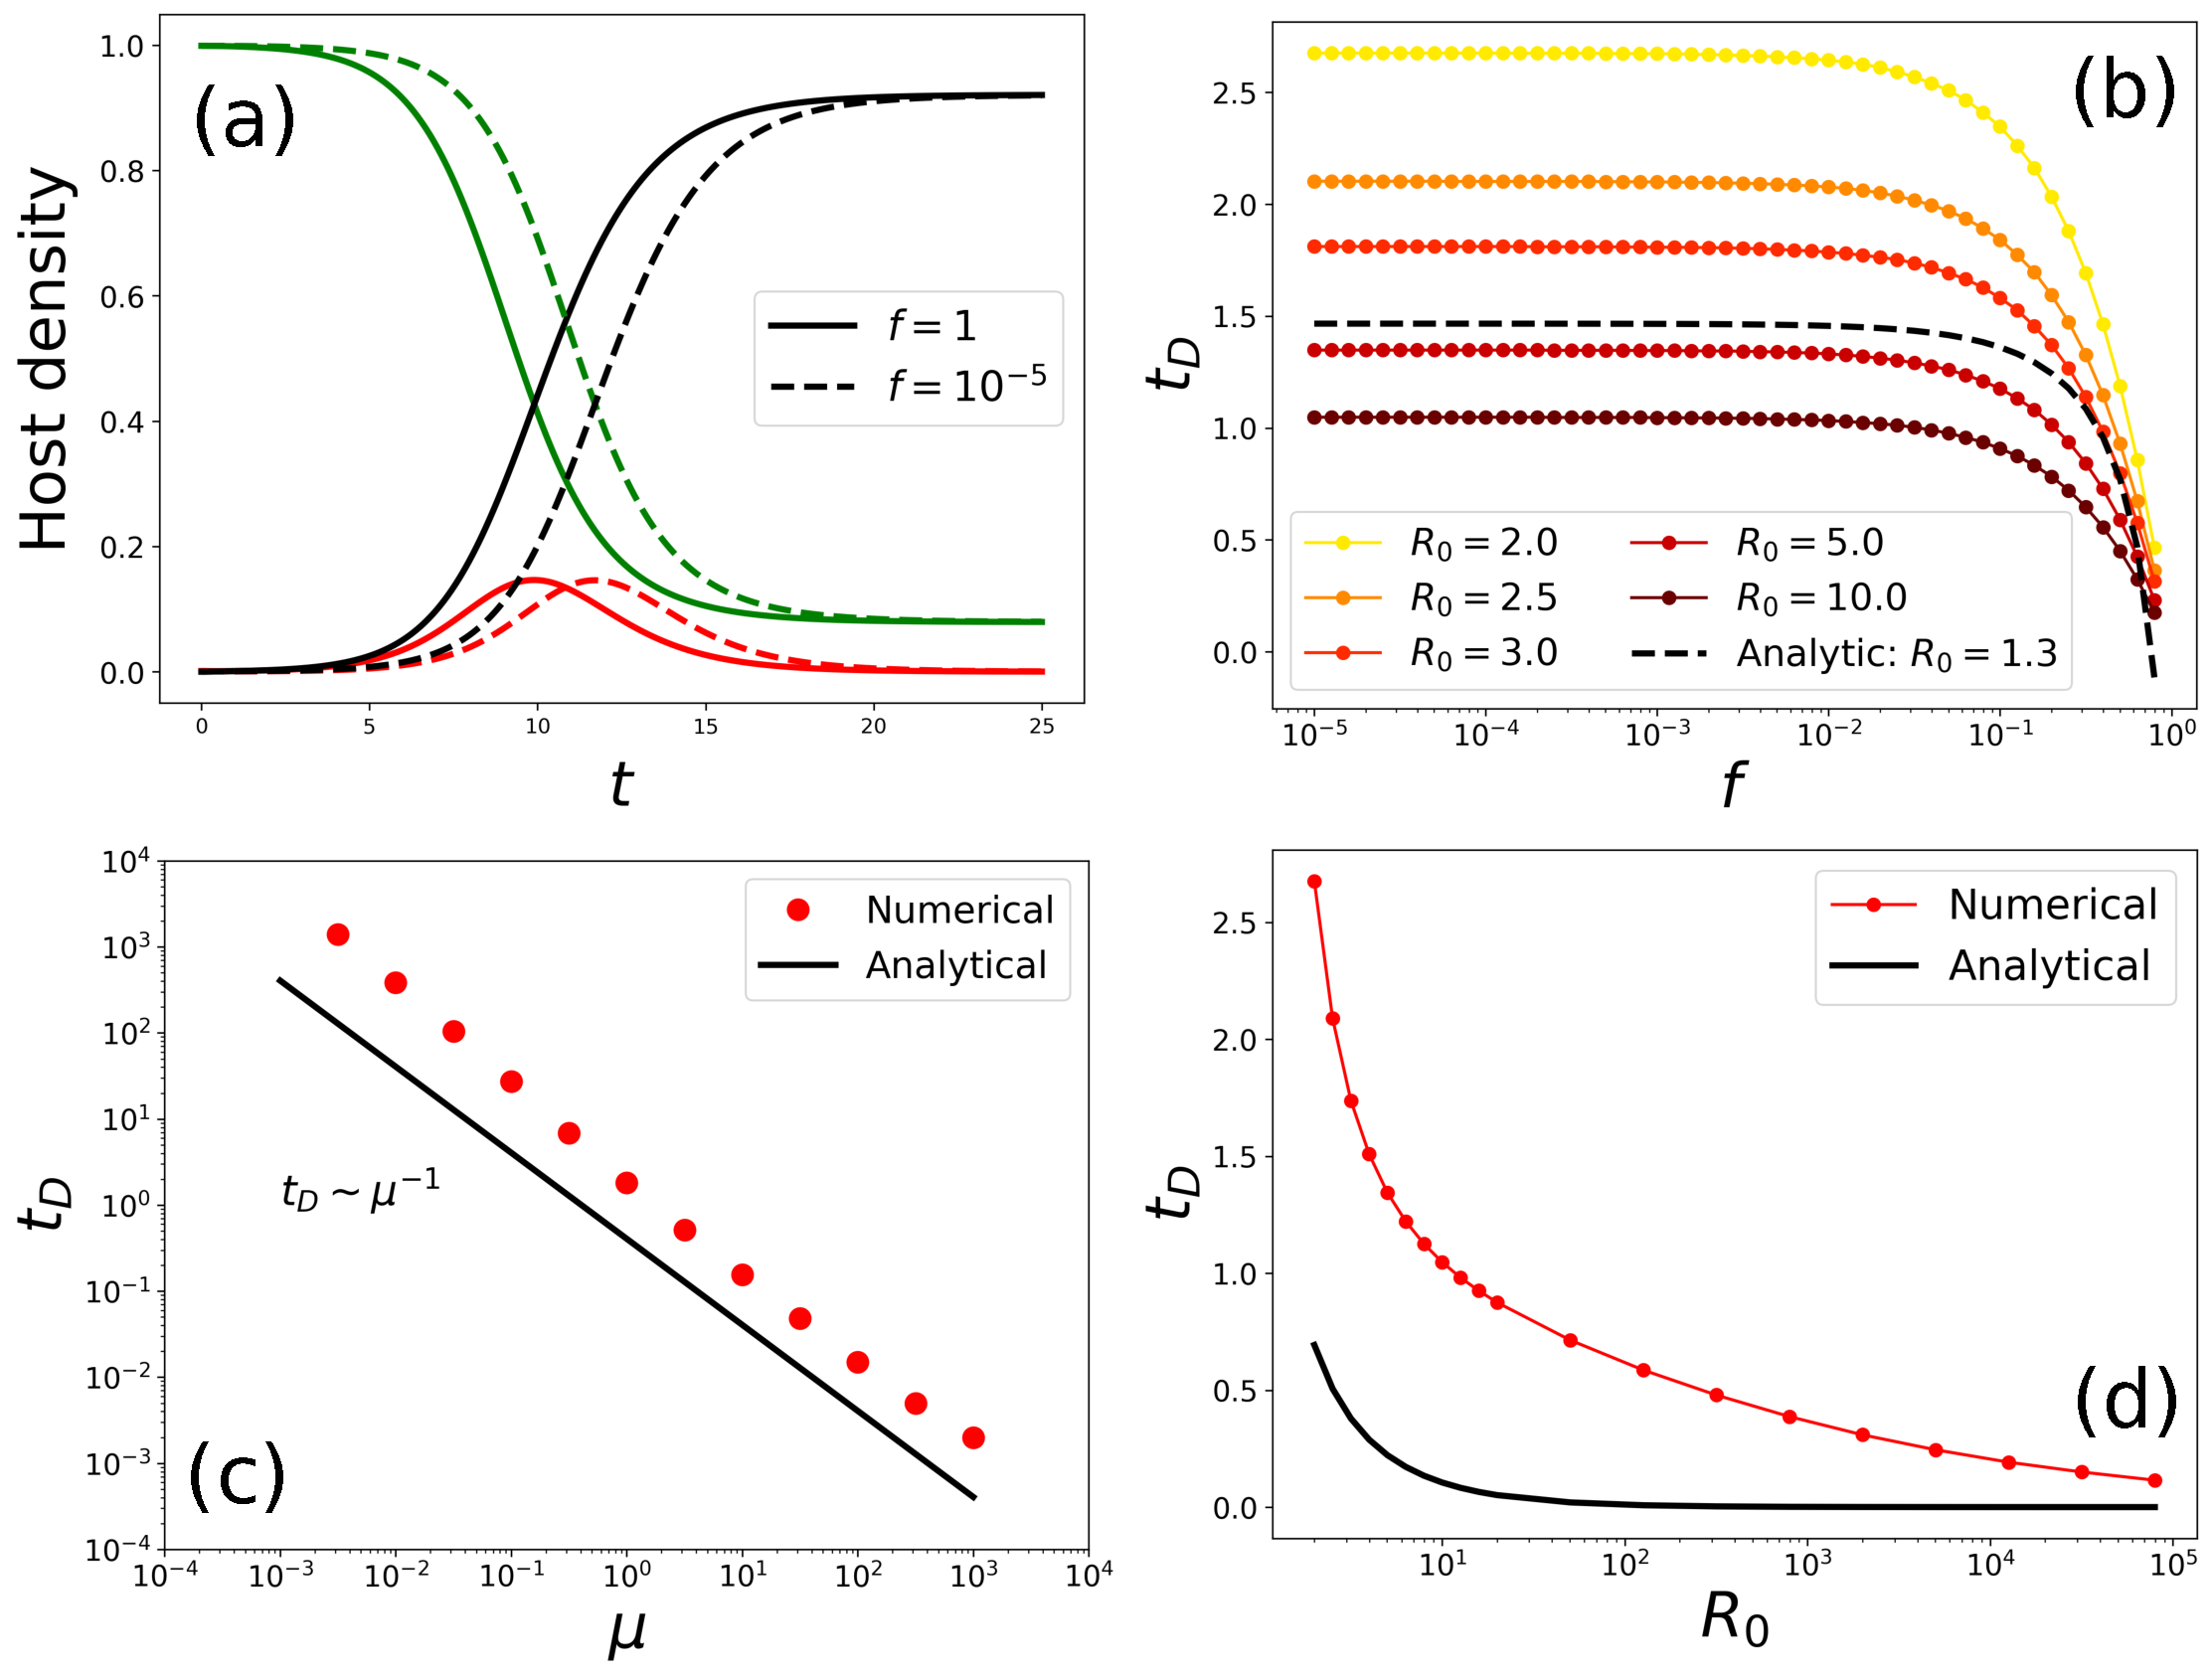
\includegraphics[width=0.8\textwidth]{Figures/delay.pdf}
    \caption{Numerical study of the delay induced by growing vector
    populations. (a) Comparison of hosts dynamics for a stationary vector
    population ($f=1$) and a growing vector population ($f=10^{-5}$). (b) Time
    delay as function of $f$ for different values of the basic reproduction
    number
    $R_0$. (c) Time delay as function of the vector natural death rate. (d)
    Time
    delay as function of the basic reproduction number, $R_0$, with
    $f=10^{-5}$.}
    \label{fig:delay}
\end{figure}

\subsection{The basic reproduction number for non-stationary vector
    populations}

As shown in the previous section, traditional methods to compute the basic
reproduction number fail in the case of epidemic models with decaying vector
populations, $f>1$, unless the time scale of vector population fulfills the
strong inequality condition \cref{eq:timescales_condition}, as illustrated in
\cref{sec:R0statvp}. Here we introduce an effective, average definition of
$R_0$, useful to predict the epidemic onset for vector-borne diseases with
decaying vector populations, i.e. the case where traditional methods fail. It
is defined as the \textit{average} number of infections produced by an infected
individual in \textit{one generation} \cref{eq:generationtime},
\begin{equation}\label{eq:R0_non_stationary}
    \overline{R_0}=\avg{R_{0}^{i}(t)}\Big\rvert\limitss{0}{t_g}=
    R_0\claudator{1-\frac{1}{\tau}\parentesi{f-1}
        \parentesi{e^{-\tau}-1}}=R_0\cdot\mathcal{F}
\end{equation}
where $\tau=1+\mu/\gamma$ and $\mathcal{F}$ accounts for the effect of the
decaying vector population on the stationary $R_0$ (see
\cref{app:R0_non_stationary} for the full derivation of
\cref{eq:R0_non_stationary}).

A first observation is that $\overline{R_0}>R_0$ always (for $f>1$). This
stems from the fact that $\tau=1+\mu/\gamma>1$, so that $e^{-\tau}-1<0$, and
$f-1>0$, which yields $\mathcal{F}>1$. This discussion unravels why standard
methods fail to predict the onset of an epidemic under decaying vector
populations. Another important point is that if $\mu/\gamma\gg 1$, which
implies $\tau\gg1$,
\begin{equation}
    \lim_{\tau\gg1}\mathcal{F}=\lim_{\tau\gg1}\claudator{1-\frac{1}{\tau}
        \parentesi{f-1}\parentesi{e^{-\tau}-1}}=1+\frac{f-1}{\tau}\
    ,
\end{equation}
and if furthermore $\tau\sim\frac{\mu}{\gamma}\gg (f-1)$ then
$\mathcal{F}\to 1$ and $\overline{R_0}\to R_0$. This is in agreement with the
discussion in \cref{sec:R0statvp} showing that the $R_0$ computed from standard
methods works if $\mu\gg\gamma$.

\begin{figure}[H]
    \centering
    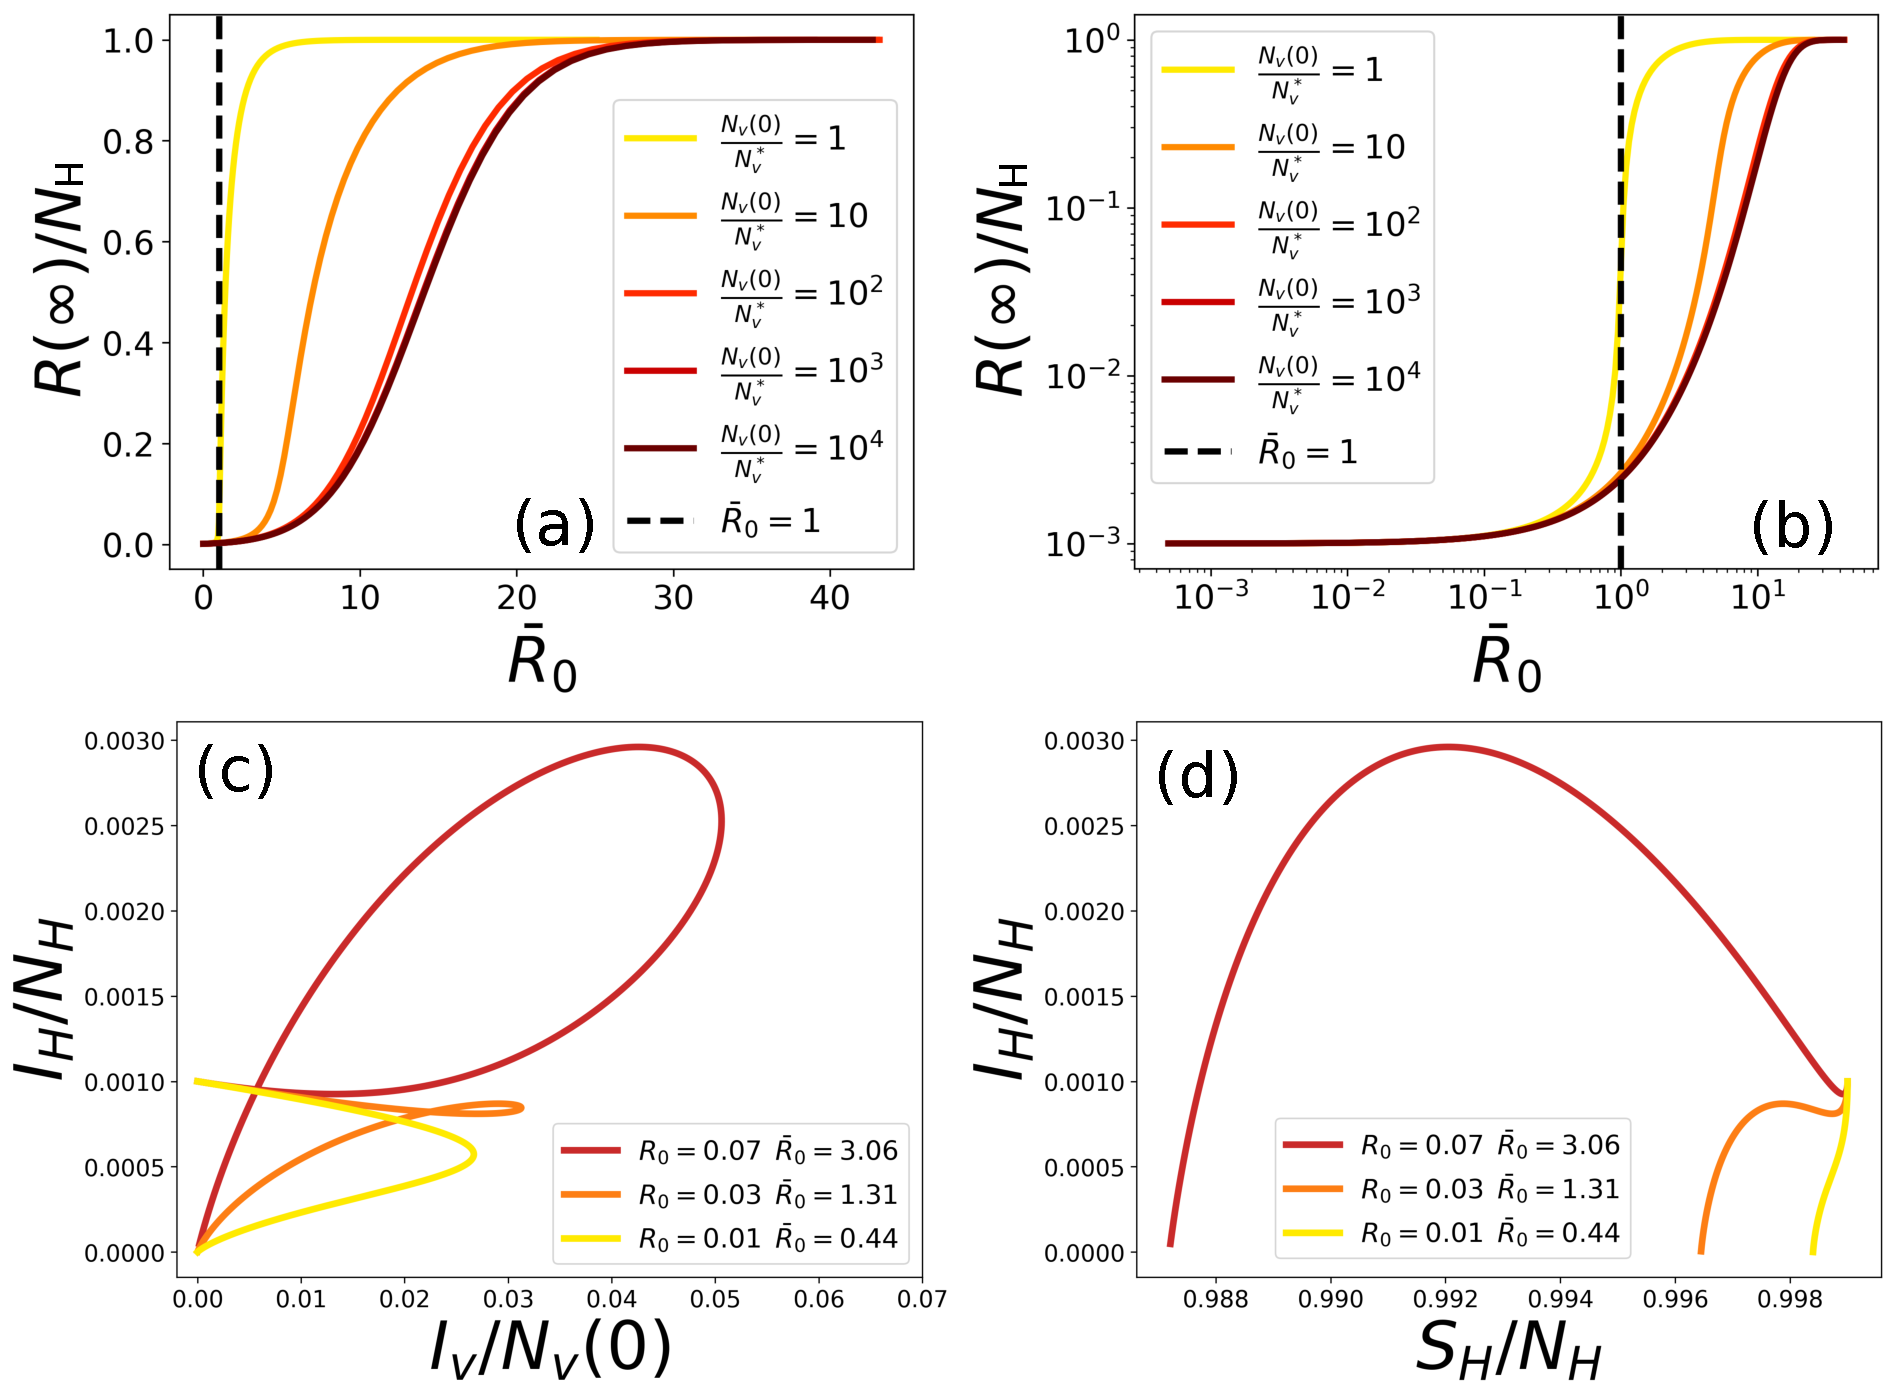
\includegraphics[width=0.8\textwidth]{Figures/R0_check_mean_value.pdf}
    \caption{Numerical verification of the expression for the basic
        reproduction number for vector-borne diseases with decaying vector
        populations
        \cref{eq:R0_non_stationary}. Final size of the epidemic as a function
        of the
        basic reproduction number in panels: (a) linear scale; (b) logarithmic
        scale.
        Phase space trajectories in panels: (c) $I_H/N_H$ vs $I_v/N_v(0)$ and
        (d)
        $I_H/N_H$ vs $S_H/N_H$, where an initial condition $I_H(0)/N_H=0.01,
            S_H(0)/N_H=0.99$ and $I_v(0)/N_V(0)=0$ has been used for the $3$
        cases.
        $\mu=\gamma$ has been used in all the simulations.}
    \label{fig:R0_check_mean_value}
\end{figure}

\cref{fig:R0_check_mean_value}(a-b) contrasts numerically the validity of
\cref{eq:R0_non_stationary} to predict the final size of the epidemic as a
function of the general basic reproduction number, $\overline{R_0}$, in linear
and logarithmic scale, respectively. We observe that, independently of the
initial condition of vectors, the outbreak occurs for $\overline{R_0}>1$.
However, we may notice that for large values of the initial condition of
vectors the final size of the epidemic grows more slowly, so that larger values
of $\overline{R_0}$ are needed to produce a proper outbreak. This can be
explained by the fact that for $\overline{R_0}$ slightly above the threshold,
$\overline{R_0}=1$, and large values of $f=N_v(0)/N_v^*$, infections are
produced only in the transient period of the dynamics, as $R_0<1$. This is,
while the vector population is decaying to its stationary value, the vectors
are able to produce new infections, but once the vector population reaches the
stationary value, the epidemics stops. This transmission mechanism is radically
different to that of vector-borne diseases with stationary vector populations
in which the pre-pandemic disease-free state is an equilibrium of the system.
The phase-space plots in \cref{fig:R0_check_mean_value}(c-d) show that the
time-averaged basic reproduction number $\overline{R_0}$ is able to accurately
predict the conditions under which the infected host population will grow, in
contrast with $R_0$ computed in the post-pandemic fixed point. In essence, for
$\overline{R_0}>1$ the infected host population, $I_H$, grows before reaching
the absorbing state, $I_H=I_v=0$, while for $\overline{R_0}<1$ the infected
host population is monotonically decreasing. We note that
\cref{eq:R0_non_stationary} is similar to the time-averaged basic reproduction
number presented in \cite{Wesley2009} for the periodic case, which is a
first-order approximation to the \textit{true} basic reproductive number
\cite{Bacaer2006}.

\subsection{Fast-slow approximation}

The original $5$-D \cref{eq:SIR_v} model is certainly not amenable to
mathematical analyses due to its high phase-space dimensionality and the fact
that it depends on $4$ parameters. Moreover, in a real-case application, if the
parameters conforming the model are not known, the model could suffer from
parameter unidentifiability. However, some approximations can be performed to
reduce the mathematical complexity of the model, as for instance a fast-slow
(or adiabatic) approximation.

If the time-scale of the vector population evolution is much faster than
that of the infected hosts, what is expected to be a good approximation in many
practical cases, the vector population will almost instantaneously adapt to its
stationary value. Thus, if $1/\mu\ll1/\gamma$, or equivalently if
$\gamma/\mu\ll1$, we can rewrite the time derivative of the vector infected
population as
\begin{equation}
    \epsilon\dot{I}_v=\frac{\alpha}{\mu}S_v\frac{I_H}{N_H} - I_v \ ,
\end{equation}
where time has been re-scaled to $t'\to\gamma t$ and $\epsilon=\gamma/\mu$
is a small parameter. Then, $\dot{I_v}$ can be neglected and the infected
vector population can be obtained from the relationship,
\begin{equation}\label{eq:Iv_timescale_approx}
    I_v\approx\frac{\alpha}{\mu}\frac{S_v I_H}{N_H} \ .
\end{equation}

Substituting \cref{eq:Iv_timescale_approx} into the original system
\cref{eq:SIR_v} and the identity $N_v(t)=S_v(t)+I_v(t)$, while considering that
the conditions for which the time-scale approximation is valid, $\mu\gg\gamma$,
imply that the vector population will reach its stationary value almost
instantaneously, so that $N_v(t)\approx N_v^*$, we obtain the following reduced
system,
\begin{equation}\label{eq:SIR_like}
    \begin{aligned}
        \dot{S}_H & =-\beta'\frac{S_H I_H}{\lambda N_H + I_H}            \\
        \dot{I}_H & =\beta'\frac{S_H I_H}{\lambda N_H + I_H}- \gamma I_H \\
        \dot{R}_H & =\gamma I_H \ ,
    \end{aligned}
\end{equation}
where $\beta'=\beta N_v^*/N_H$ and $\lambda=\mu/\alpha$.

Moreover, if $f\neq1$ the above mentioned timescales relationship
must fulfil
$\displaystyle\frac{\mu}{\gamma}\gg\abs{\ln{\frac{\epsilon}{f-1}}}$ (cf.
\cref{eq:timescales_condition}) and not only
$\displaystyle\frac{\mu}{\gamma}\gg 1$. It is important to notice that the
presence of direct host to host transmission would simply re-scale the
coefficient $\beta'$, and the SIR reduction \cref{eq:SIR_like} would keep its
validity.

\begin{figure}[H]
    \centering
    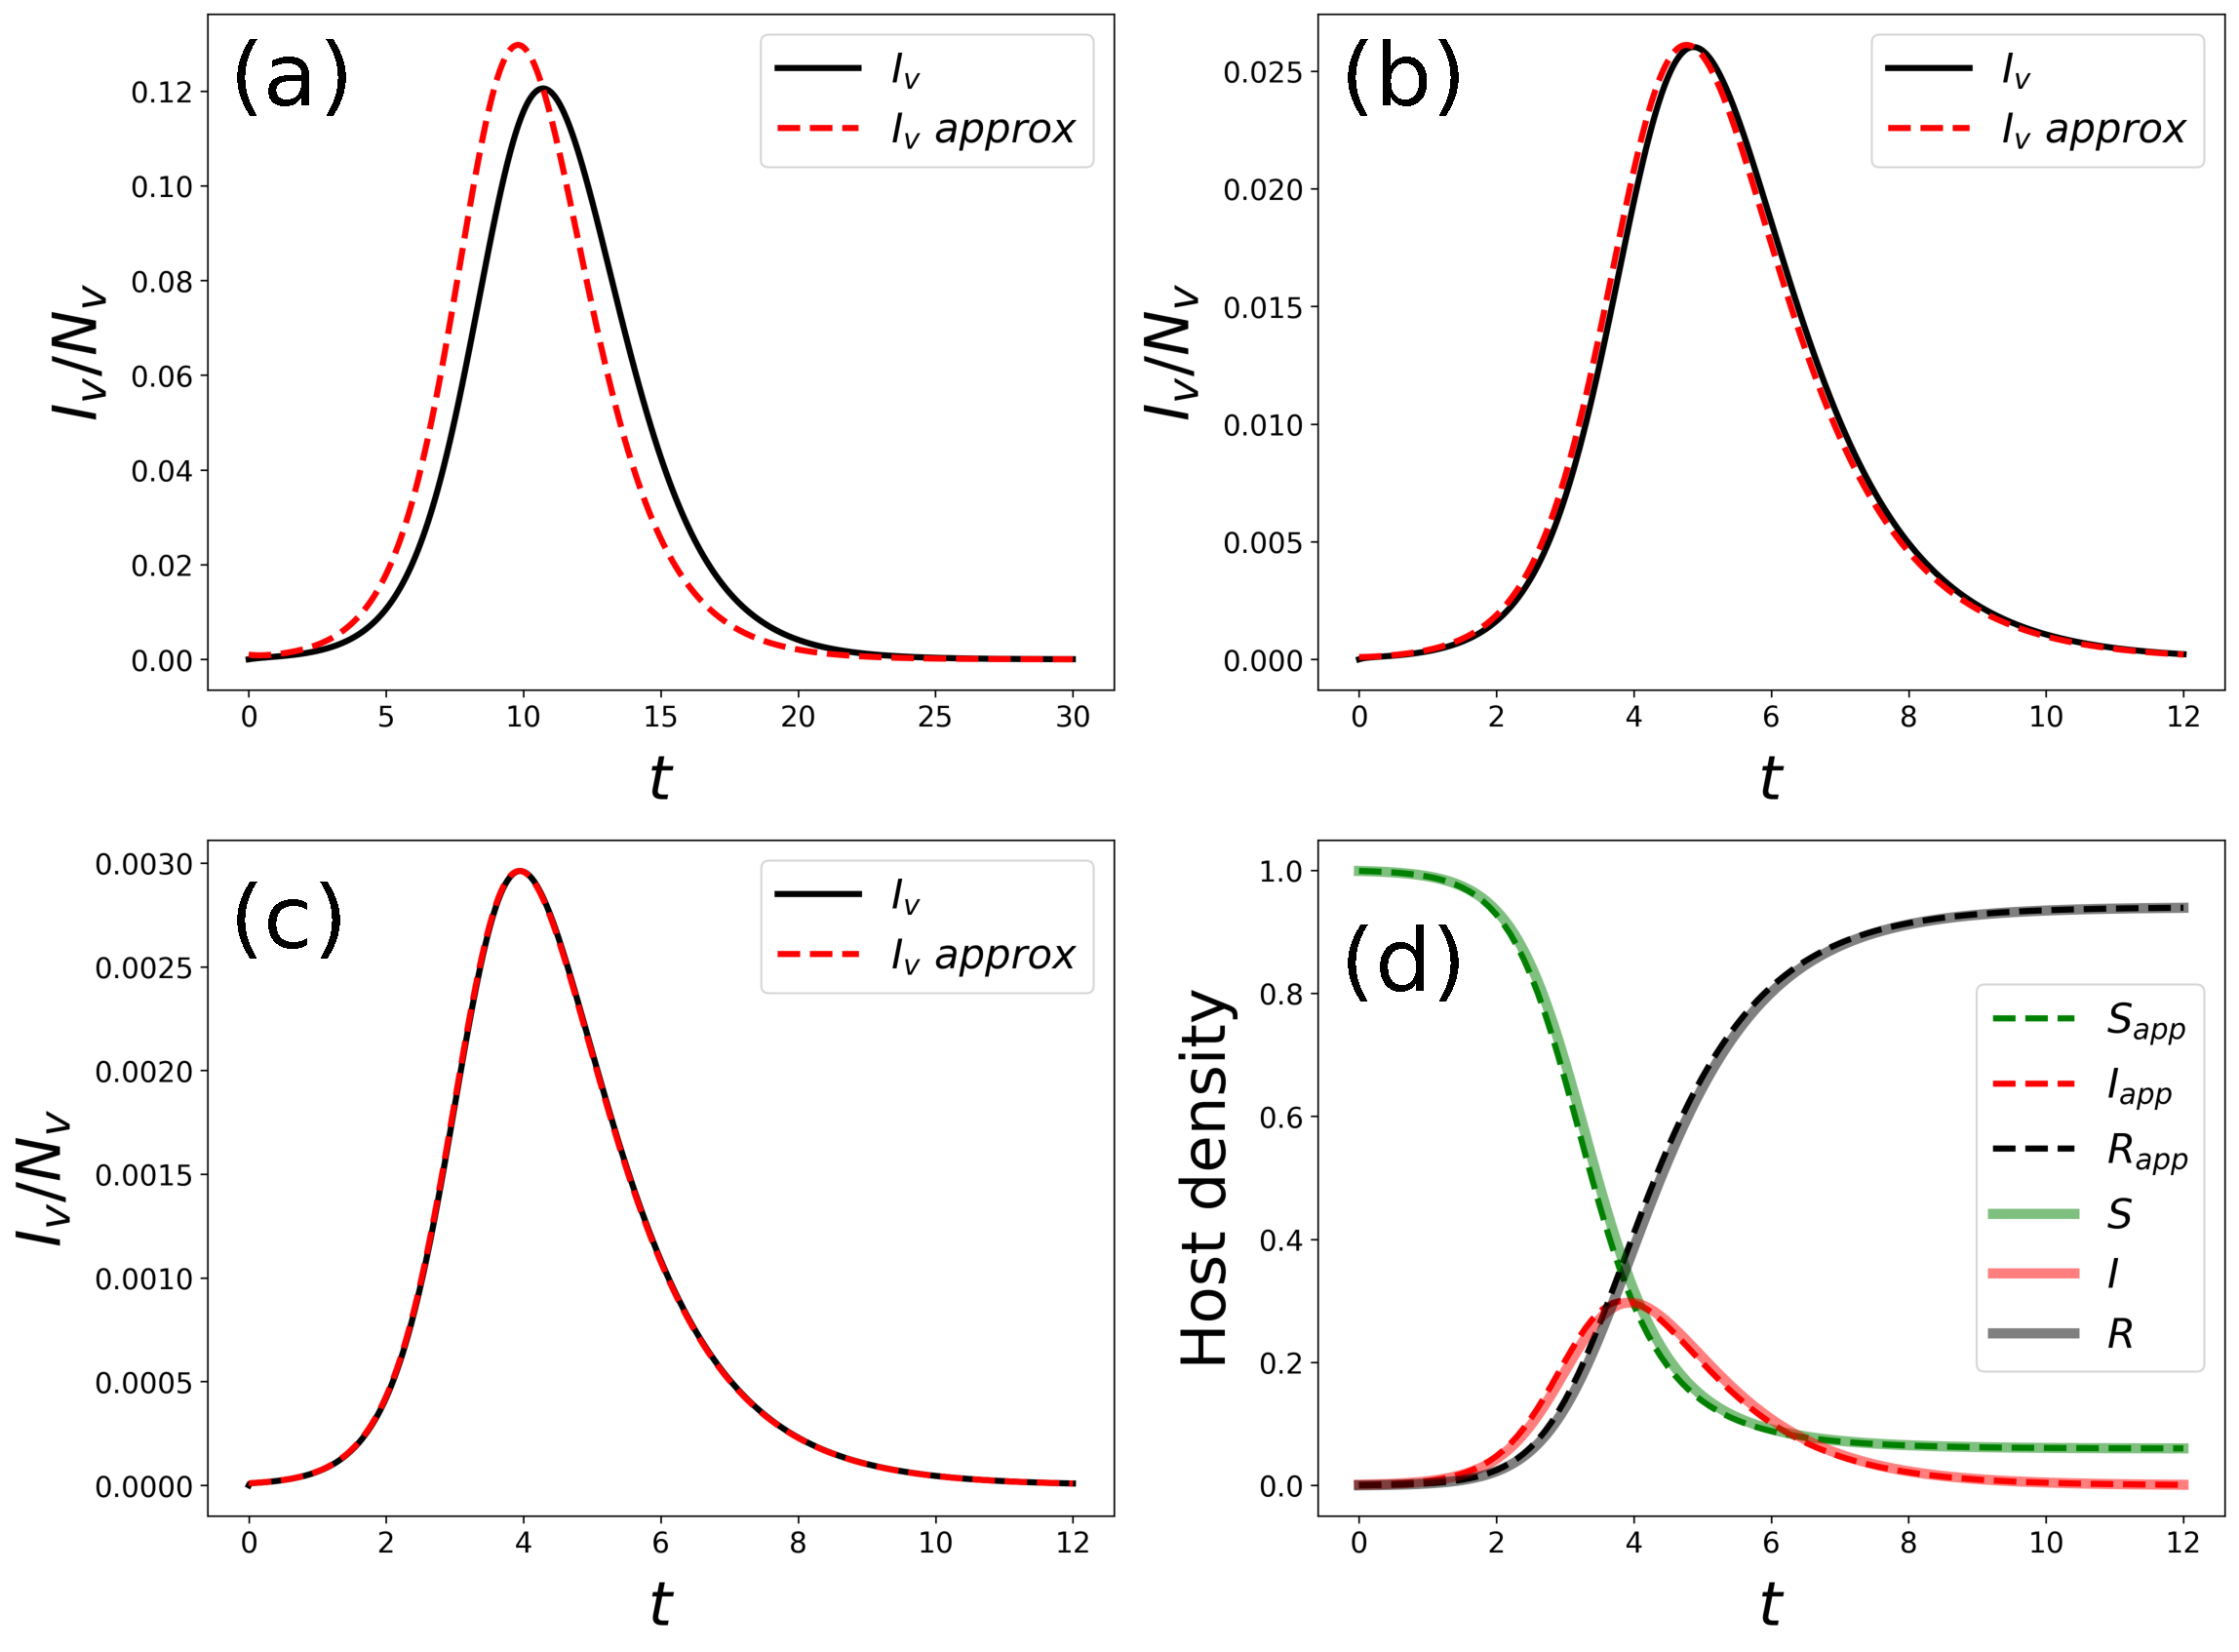
\includegraphics[width=0.8\textwidth]{Figures/Timescale_approx.pdf}
    \caption{Numerical verification of the time-scale approximation
        (\cref{eq:Iv_timescale_approx}) with $N_H=100$, $\alpha=\gamma=1$.
        $\beta$ is
        chosen such that $R_0=3$. (a) $\mu=1$, (b) $\mu=10$, (c) $\mu=100$.
        Panel (d)
        shows a comparison between the approximate and original models for the
        parameters used in (c), where the approximated models is expected to
        represent
        well the original one.}
    \label{fig:timescale_approx}
\end{figure}

In \cref{fig:timescale_approx} we numerically verify the validity of the
presented fast-slow approximation. As expected, we observe that the
approximation breaks down for $\mu\sim\gamma$ (\cref{fig:timescale_approx}(a)),
while as
$\mu$ becomes larger than $\gamma$ the approximation improves
\cref{fig:timescale_approx}(b) and it becomes quantitative when $\mu\gg\gamma$,
\cref{fig:timescale_approx}(c). Finally, we show in
\cref{fig:timescale_approx}(d) a comparison between the dynamics of the hosts
using both the original and the approximated model using the same parameters
than in \cref{fig:timescale_approx}(c), where the results of both models are
expected to converge.

\subsection{Reduction to a SIR model}

In addition to the previous condition, $\gamma/\mu\ll1$, if one has that
$\lambda N_H \gg I_H$ also holds (which is indeed plausible in this limit)
\cref{eq:SIR_like}, then the model can be written as a standard SIR model,
\begin{equation}\label{eq:SIR}
    \begin{aligned}
        \dot{S}_H & =-\beta_{eff}\frac{S_HI_H}{N_H}            \\
        \dot{I}_H & =\beta_{eff}\frac{S_HI_H}{N_H}- \gamma I_H \\
        \dot{R}_H & =\gamma I_H \ ,
    \end{aligned}
\end{equation}
where $\displaystyle\beta_{eff}=\frac{\beta'}{\lambda}=\frac{\beta\alpha
        N_v^*}{\mu N_H}$.

\begin{figure*}[t!]
    \centering
    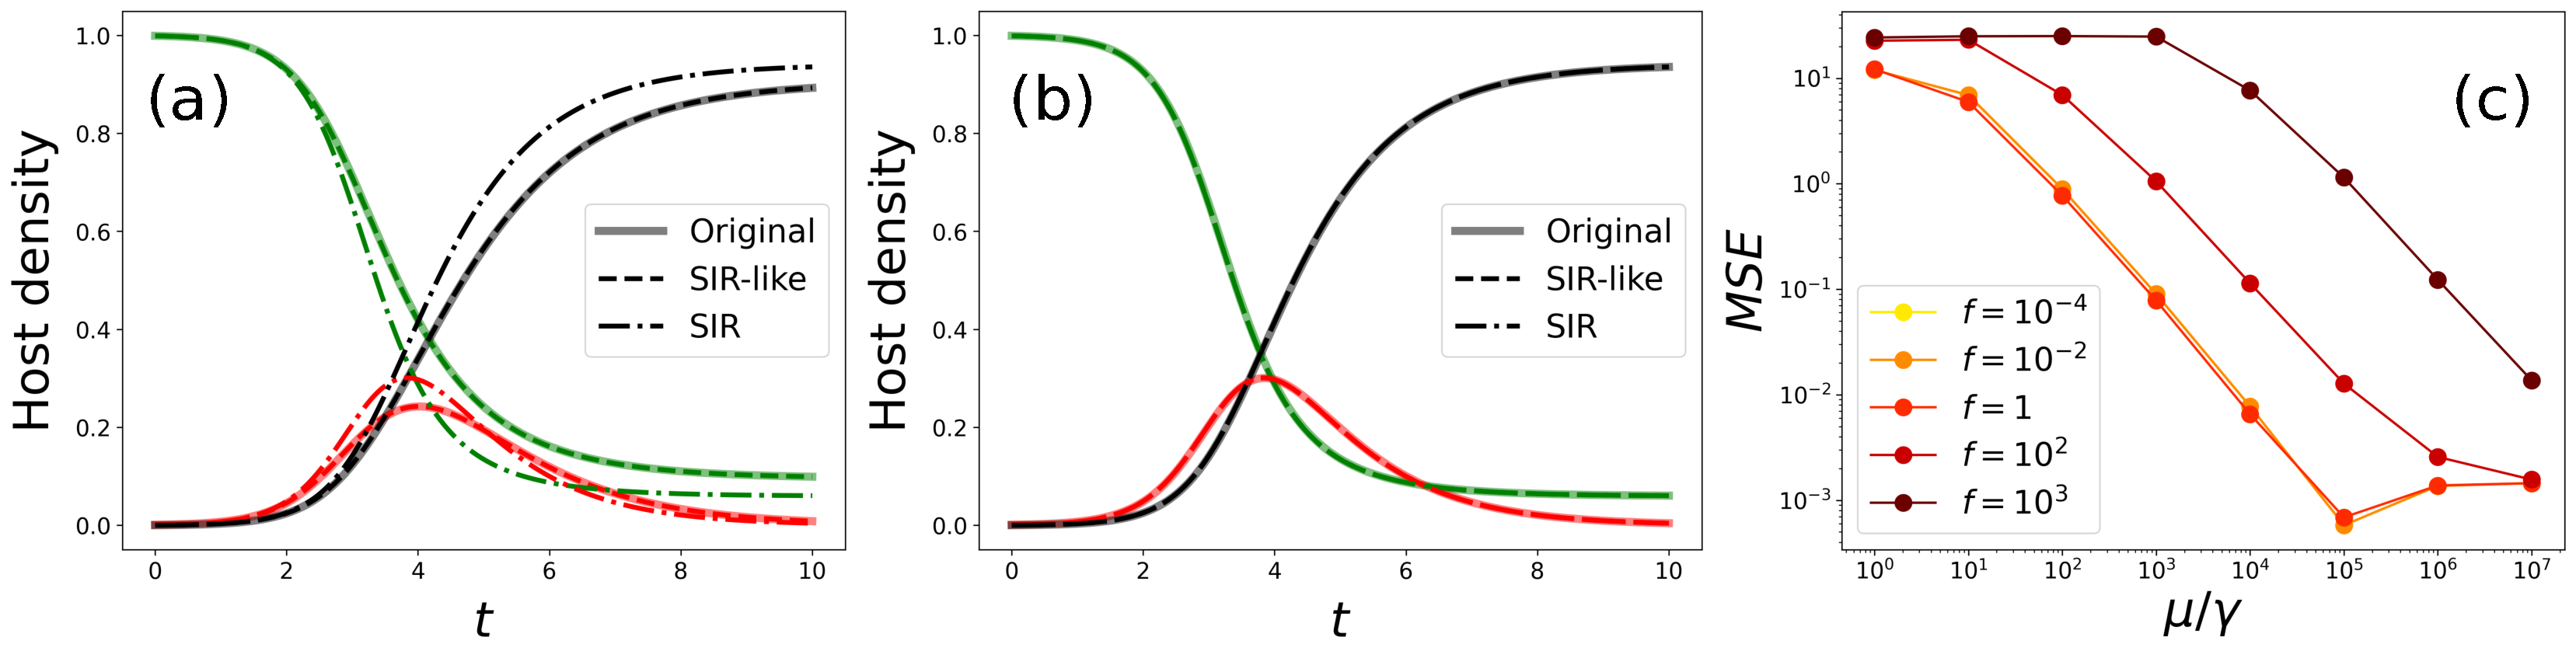
\includegraphics[width=\textwidth]{Figures/SIR_like_approx_comp.pdf}
    \caption{Comparison between the original model and the reductions,
    \cref{eq:SIR_like} (SIR-like) and \cref{eq:SIR} (SIR) with $N=100$,
    $\mu/\gamma=10^{3}$ and $f=1$. $\beta$ was chosen such that $R_0=3$.  (a)
    $\lambda=1$, (b) $\lambda=10^3$, (c) Mean Squared Error between the
    original
    model and the SIR approximations as function of the ratio $\mu/\gamma$ and
    $f$.}
    \label{fig:SIR_like_approx}
\end{figure*}

In \cref{fig:SIR_like_approx} we show the validity of the reduced models
\cref{eq:SIR_like} and \cref{eq:SIR}. \cref{fig:SIR_like_approx}(a) shows that
the SIR-like model (\cref{eq:SIR_like}) works when the time-scale approximation
can be performed (as $\mu/\gamma\gg1$) but the SIR model fails when the
condition $\lambda N_H \gg I_H$ is not fulfilled. Conversely, in
\cref{fig:SIR_like_approx}(b) we show that as $\lambda N_H \gg I_H$ is
fulfilled, then the SIR model perfectly matches the original model. Finally,
\cref{fig:SIR_like_approx}(c) shows the decrease in the mean squared error of
the approximation as the condition \cref{eq:timescales_condition} is fulfilled
for different values of $f$.

\section{Conclusions}\label{sec:conclusions}

In the present work we have analyzed several features of a compartmental
deterministic model for vector-borne diseases with $3$ compartments for hosts
and $2$ for vectors, that does not consider neither direct host to host nor
vertical transmission. The goal is to study the behavior of the model in the
case that the vector population is not stationary. In this case, the
pre-pandemic disease-free state is not a fixed point (equilibrium state) of the
dynamical system, and, in principle, the methods that are customarily used to
determine the basic reproduction number, $R_0$ do not work. This is so because
these methods determine the onset of an outbreak by performing a linear
stability analysis of the disease-free state, assuming that it is a fixed point
of the model. A common assumption made in the literature is to determine $R_0$
from the asymptotic state for the vectors (if it is not an extinction state), a
fixed point of the model.

We have analyzed several initial conditions of the vector population,
characterizing different regimes. In the case that the initial condition for
the number of vectors is below the asymptotic state, implying that the vector
population overall grows, then $R_0$ as determined from the asymptotic state
correctly predicts the existence (or not) of an epidemic outbreak, but with a
temporal delay in its appearance. This result contrasts with the situation in
which the initial state is above the asymptotic state, with an overall decrease
in the vector population. In this case $R_0$ determined from the asymptotic
state may fail badly, predicting no outbreak while a large fraction of the
population might get infected. We present a simple, albeit useful,
generalization of $R_0$ that is able to give a reasonable prediction of the
epidemic threshold for decaying populations, including the case in which
vectors become extinct, a case in which the asymptotic estimation to determine
$R_0$ cannot be applied.

Compartmental models of vector-borne diseases usually have many
compartments and parameters, which can lead to a problem of parameter
unidentifiability. The model analyzed here is not an exception, and when
applied to real-world cases many different combinations of the parameters could
be able to reproduce the available data. Thus, in order to facilitate the
application of the model to experimental data, we have studied a useful
fast-slow (or adiabatic) approximation that allows to reduce the model if the
parameters fulfill certain conditions. In particular, our study shows that
under quite realistic assumptions (the typical timescale of hosts infection and
death is much slower than vector timescales) it is possible to obtain a reduced
SIR model. We recall that this reduction implies that, under these assumptions,
the process by which hosts (that could be immobile) get infected through the
action of vectors is equivalent to a direct interaction among hosts.

The deterministic compartmental model analyzed here, with some
modifications, is a clear candidate to study many vector-borne diseases, in
particular phytopathologies. Furthermore, in case of parameter
unidientifiability the model reductions performed in this work could be useful
to solve this issue. In any case, this description is still idealized, as
compartmental models imply a well-mixed assumption in which space is not
explicitly described. This kind of representations are not always applicable to
real-world scenarios although are useful as a first approximation. Thus, future
research should focus on the integration of space and vector mobility in the
model to account for more realistic situations.

%----------------------------------------------------------------------------------------
%	A compartmental model for Xylella fastidiosa diseases with explicit
%   vector seasonal dynamics
%----------------------------------------------------------------------------------------
\chapterimage{almond.jpg}
\chapterspaceabove{6.75cm}
\chapterspacebelow{7.25cm}

\chapter{A compartmental model for \textit{Xylella fastidiosa} diseases with
  explicit vector seasonal dynamics}
\vspace{3cm}

% \textbf{Àlex Giménez-Romero$^{1}$, Eduardo Moralejo$^{2}$, Manuel A.
%     Matías$^{1}$}

% \vspace{1cm}

% \begin{enumerate}
%     \small
%     \item Instituto de Física Interdisciplinar y Sistemas Complejos, IFISC
%           (CSIC-UIB), Palma de Mallorca 07122, Spain
%     \item Tragsa, Passatge Cala Figuera 6, 07009 Palma de Mallorca, Spain
% \end{enumerate}

% \vspace{1cm}

\textbf{Published as}

\vspace{0.5cm}

\fullcite{GimenezRomero2023}

\newpage
\section{Introduction}

Mathematical and computational modeling in Ecology and, in particular,
Epidemiology have been recently recognized as powerful approaches to guide
empirical work and provide a framework for the synthesis, analysis and
development of conservation plans and policy-making
\cite{levin1992mathematics,Murray_book,sarkar2006biodiversity,Chew2014}.
Plant epidemics, mainly plant-virus diseases, have been often described by
compartmental models, which deal with the overriding importance of transmission
mechanisms in determining epidemic dynamics
\cite{Jeger1998,Jeger2004,Madden2000}. These models have contributed to
providing answers to some questions related to the ecology of plant diseases
and have led to direct applications in disease control while guiding research
directions \cite{Jeger2019}.

The emergence of vector-borne plant pathogens in new areas causing huge
economic impacts, such as \textit{Xylella fastidiosa} and the
\textit{Candidatus} Liberibacter spp. (Huanglongbing or citrus greening), has
sparked interest in modeling vector-transmitted plant-disease epidemics
\cite{chiyaka2012modeling,Jeger2019}. The vector-borne bacterium \textit{X.
    fastidiosa} (Xf) is a multi-host pathogen endemic to the Americas that
causes
economically important diseases, mostly in woody crops \cite{Hopkins2002}. Xf
is a genetically diverse species with three evolutionary well-defined clades
forming the \textit{pauca}, \textit{fastidiosa}, and \textit{multiplex}
subspecies, native from South, Central, and North America, respectively
\cite{vanhove2019genomic}. Within each subspecies, diverse genetic lineages
with different host ranges are found. Xf is transmitted non-specifically by
xylem-sap-feeding insects belonging to the sharpshooter leafhoppers (Hemiptera:
Cicadellidae, Cicadellinae) and spittlebugs (Hemiptera: Cercopoidae)
\cite{Redak2004}.

Recently, Xf has gained renewed interest due to the massive mortality of
olive trees in Apulia, Italy \cite{saponari2019xylella}. The first focus of
the olive quick decline syndrome (OQDS) was detected in 2013 around Gallipoli
(Apulia, Italy)\cite{saponari2013identification} and since then has spread
throughout the region by the meadow spittlebug, \textit{Philaenus spumarius}.
Although this was the first official detection of Xf in Europe, it has recently
been demonstrated that the pathogen arrived much earlier in Corsica
\cite{Soubeyrand2018} and in the Balearic islands \cite{Moralejo2020}.
Around 1993, two strains of the subspecies \textit{fastidiosa} (ST1) and
\textit{multiplex} (ST81) were introduced from California to Mallorca (Spain)
with infected almond plants \cite{Moralejo2020}. To date, over 80\% of the
almond trees in Mallorca show leaf scorch symptoms and the outbreak has changed
the iconic rural landscape of this Mediterranean island \cite{Olmo2021b}.

The meadow spittlebug,	\textit{P. spumarius} (Hemiptera: Aphrophoridae),
has recently been shown to be the main vector of Xf in Europe both in
transmission experiments and in field studies
\cite{Cornara2017,Cornara2018,lopez2022mechanical,Moralejo2019,saponari2019xylella}.
\textit{P. spumarius} is a polyphagous species from the Palearctic region,
presenting one generation per year (univoltine) and overwintering as eggs.
Foam-forming nymphs emerge at the end of winter, feeding on herbaceous plants.
The time required for their development to the adult stage depends mainly on
temperature and humidity
\cite{bodino2019phenology,Chmiel1979,cornara2018philaenus}. In Mediterranean
climates,  \textit{P. spumarius} adults generally move from the herbaceous
cover to the crop canopy as evapotranspiration increases in late spring
(May–June). In mid-summer, the populations of \textit{P. spumarius} tend to
decrease in the crop canopy, while the insects are captured more frequently in
trees and shrubs interspersed in crops. Summer dispersal of spittlebugs to wild
hosts as refugee seems a common general pattern in Mediterranean crops in Italy
\cite{bodino2019phenology,cornara2021natural} and Spain
\cite{morente2018distribution}. Because the bacterium has not been detected
in spring on insects feeding on the herbaceous cover or in weeds in Europe
\cite{bodino2019phenology,cornara2018philaenus,Olmo2021b}, it is assumed that
all spittlebug adults acquire the bacteria from the main crop (olive, almond,
vine, etc.). Once infected, Xf colonizes the insect foregut in a persistent and
non-circulatory manner without transovarial (parent to offspring) or
transstadial (inter-stage) transmission
\cite{Almeida2003,freitag1951host,purcell1979evidence} and without
a period latency after vector acquisition \cite{Almeida2015,freitag1951host}.

Several epidemic models have been already developed for Xf-diseases, but
they lack a realistic description of some relevant processes
\cite{Jeger2019}. Some of these models assume a simple general form for
infected host dynamics \cite{White2017,Abboud2019,Daugherty2019} or use a
simplified S-I compartmental scheme for hosts, disregarding important features
such as the latent period or the host mortality rate \cite{Soubeyrand2018}.
Models that do take these features into account, however, do not explicitly
model the population of vectors responsible for disease transmission
\cite{White2020}. Other more recent models have taken a step further in
explicitly modeling the vector population \cite{BRUNETTI2020,
    GimenezRomero2022_CommsBio}, but the characterization of its dynamics is
still
relatively simple, as it overlooks the known seasonal patterns of vector
abundance. Several recent studies have provided new insights into the ecology
and temporal dynamics of the transmission of Xf by \textit{P. spumarius} in
olive plants \cite{Bodino2021,bodino2019phenology}. However, these
experimental data of the pathosystem have not been yet integrated at the
population level. Thus, there is a need to continue advancing in the modeling
of Xf diseases by developing more realistic models that can elucidate the
fundamental processes involved in vector-host-pathogen interactions and help to
design effective control strategies.

In this work, we develop a deterministic continuous-time compartmental
model to describe the general epidemiological dynamics of diseases produced by
Xf in Europe. We explicitly account for key biological aspects of the disease,
including the seasonal dynamics of its main vector, \textit{P. spumarius}. Our
model is able to describe field data from the two major European outbreaks: the
olive quick disease syndrome (OQDS) in Apulia, Italy, caused by the subspecies
\textit{pauca}, and the almond leaf scorch disease (ALSD) in Mallorca, Spain,
caused by subspecies \textit{multiplex} and \textit{fastidiosa}. We aimed to
find the most influential parameters in the model with respect to incidence and
mortality in both diseases by performing a global sensibility analysis. With
this information, the next goal was to explore control strategies acting
especially on the vector population.

\section{Materials and Methods}

\subsection{Epidemic model: the SEIR-V model}

We developed a deterministic continuous-time compartmental model that
incorporates the specific biological features of Xf diseases in Europe,
including the dynamics of the main relevant vector \textit{P. spumarius}
\cite{Cavalieri2019}. To build the model we took the following
considerations: (i) we assume there is no winter recovery of infected hosts and
thus they die sometime after infection; (ii) hosts show an asymptomatic period
in which they are non-infectious in practice (exposed compartment) because the
bacteria are not yet systemically extended
\cite{teviotdale2003almond,Stevenson238}, while vectors are infectious
immediately after acquiring the bacterium \cite{Fierro2019}; (iii) vectors
have an annual life cycle without mother-to-offspring disease transmission
\cite{freitag1951host,purcell1979evidence}, so we consider the annual
emergence of susceptible newborn vectors and a constant death rate for both
susceptible and infected vectors; (iv) infected vectors carry the bacterium
during their entire lifespan without affecting their fitness; and finally, (v)
we do not consider host recruitment or natural death given that the typical
development time of Xf-epidemics is faster than the typical host's life cycle.

Altogether, our deterministic continuous-time compartmental model consists
of six compartments, four describing the host population (susceptible, $S_H$,
exposed, $E_H$, infectious, $I_H$, and removed, $R_H$), and two describing the
vector population (susceptible, $S_V$, and infected, $I_V$). The model is
defined according to the following processes,
\begin{equation}\label{eq:scheme_infection_phyto}
    \begin{aligned}
         & S_H+I_V \stackrel{\beta}{\rightarrow} E_H + I_V, \quad
        E_H \stackrel{\kappa}{\rightarrow} I_H, \quad
        I_H  \stackrel{\gamma}{\rightarrow} R_H                      \\
         & S_V+I_H \stackrel{\alpha}{\rightarrow} I_V+I_H, \quad S_V
        \stackrel{\mu}{\rightarrow} \varnothing, \quad I_V
        \stackrel{\mu}{\rightarrow}
        \varnothing
        \ ,
    \end{aligned}
\end{equation}
which are illustrated in \cref{fig:model_diagram_phyto}, being the birth of new
susceptible vectors described as a source term.
Thus, the host-vector compartmental model is written as,
\begin{equation}\label{eq:SEIR_v}
    \begin{aligned}
        \dot{S}_H & =-\beta S_H I_v / N_H                                   \\
        \dot{E}_H & =\beta S_H I_v / N_H - \kappa E_H                       \\
        \dot{I}_H & =\kappa E_H - \gamma I_H                                \\
        \dot{R}_H & =\gamma I_H                                             \\
        \dot{S}_v & = N_v(0)\sum_{n=1}^{\infty}\delta(t-nT) -\alpha S_v I_H
        / N_H - \mu S_v                                                     \\
        \dot{I}_v & =\alpha S_v I_H / N_H - \mu I_v \ .
    \end{aligned}
\end{equation}

\begin{figure}
    \centering
    \label{fig:model_diagram_phyto}
    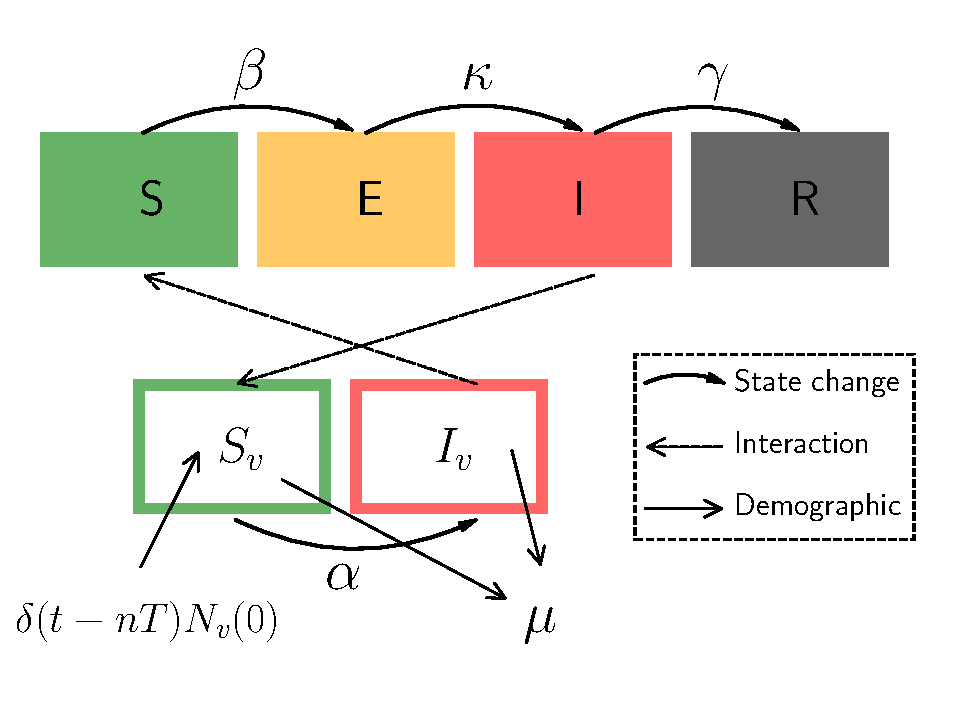
\includegraphics[width=0.8\textwidth]{Figures/SEIR_v_scheme.pdf}
    \caption[Schematic representation of the model]{Schematic representation of
        the model \cref{eq:SEIR_v}. Boxes
        are the compartments in which the population is divided, solid curved
        arrows
        represent changes in state, i.e. transitions between compartments,
        dashed
        arrows depict the crossed interaction between hosts and vectors and
        solid
        straight arrows represent demographic changes in vector population.}
\end{figure}

The model describes the exposure of susceptible hosts, $S_H$, at a rate
$\beta$ through their interaction with infected vectors, $I_v$, while
susceptible vectors, $S_v$, get infected immediately at a rate $\alpha$ through
their interaction with infectious hosts $I_H$. Exposed hosts get infectious at
rate $\kappa$, being the mean latent period $\tau_E=1/\kappa$, while infectious
hosts die at rate $\gamma$, having a mean infectious period of
$\tau_I=1/\gamma$. Infected vectors stay infected and infectious for the rest
of their lifetime. Regarding the seasonal dynamics of vectors, we assume that
new adults emerge synchronously each year in fields being all susceptible. This
is represented by the term $N_v(0)\sum_{n=1}^{\infty}\delta(t-nT)$ in
\cref{eq:SEIR_v}, where $T=\SI{1}{yr}$ is the period and $\delta(t-nT)$ is
Dirac delta function, and basically implements a yearly pulse of new vectors at
a certain moment in the year. Vectors are removed (die, move to herbaceous
vegetation and other non-host trees, exit the field, etc) at a given rate
$\mu$, which we consider identical for susceptible and infected vectors. For
simplicity, we consider that the quantity of annual newborn adults, $N_v(0)$,
is constant. This outburst of new adults followed by an exponential decay
resembles the temporal patterns on the abundance of \textit{P. spumarius}
observed in crop fields  \cite{Antonatos2021,Beal2021,Cornara2017,Lopez2021}
(see \cref{fig:vector_dynamics}).

In our model (\cref{eq:SEIR_v}) the crossed nonlinear terms in $\dot{S}_H$
and $\dot{S}_v$, $S_H I_v$ and $S_v I_H$, are divided by the total host
population, $N_H$. Thus, the vector-to-plant infection process is modeled using
mass action incidence, which is density dependent, while the plant-to-vector
infection process is modeled using standard incidence, which is frequency
dependent \cite{MartchevaBook}. This implies that doubling the number of
vectors in the crop field would double the number of resulting exposed (or
infected) hosts, as this process is population-dependent (mass action
incidence), while doubling the number of hosts would not result in more vectors
per unit area being infected, as this process only depends on the contact
probability, being frequency dependent (standard incidence). We think this is
the most reasonable assumption because, for a given plantation framework,
increasing the number of hosts is expected to also increase the area of the
field, while the number of vectors is an independent quantity.

\subsection{Basic reproductive number}

The basic reproductive number, $R_0$, of the model cannot be trivially
computed using standard methods such as the Next Generation Matrix (NGM)
\cite{Diekmann2010}, as there is no pre-pandemic fixed point in the system of
differential equations \cref{eq:SEIR_v}. For periodically varying vector
populations, rigorous methods have been developed \cite{Bacaer2007}, but not
for the case of growing or decaying vector populations. Here we use the simple
method developed in \cref{ch:xf_PRE} \cite{GimenezRomero2022_PRE} (see
\cref{app:R0}), which
effectively computes the average number of secondary infections produced by an
initially infectious individual in one generation. Thus, the effective basic
reproductive number is given by
\begin{equation}\label{eq:R0}
    R_0=\frac{\beta\alpha}{\mu\gamma}\frac{S_H(0)}{{N_H}^2}
    \frac{N_v(0)}{\mu\tau}\left(1-e^{-\mu\tau}\right)
    \ ,
\end{equation}
where $\tau$ corresponds to the time length of one generation, in our case
one year. This $R_0$ is calculated using the initial susceptible host
population, $S_H(0)$. Below we will also use a time-dependent $R_0(t)$ using
$S_H(t)$.

\subsection{Epidemiological data}

Epidemiological data from an ALSD outbreak in the island of Mallorca,
Balearic Islands, Spain were taken from \cite{Moralejo2020}. Dated phylogenetic
analysis and estimates of disease incidence showed that the introduction of
both subspecies occurred around 1993 and $\sim 79$\% almond trees were infected
in 2017 \cite{Moralejo2020}. The annual proportion of infected individuals in
the almond tree population between 1993 and 2017 was estimated by analyzing
through qPCR the presence of Xf-DNA in the growth rings of $34$ sampled trees
(cf. Fig. 3 in \cite{Moralejo2020}). The disease progression curve was
estimated without distinguishing whether infections were caused by
\textit{multiplex} or \textit{fastidiosa} subspecies. In addition, a two-sided
bootstrap confidence interval for each data point was set using the SciPy
bootstrap function in Python \cite{SciPy}. On the other hand, epidemic data
for OQDS were retrieved from \cite{White2020}. The data consisted of 2 to 3
yearly censuses of symptom prevalence in 17 olive groves infected with Xf
subsp. \textit{pauca} in Apulia, Italy, which were aggregated to fit our model
as shown in Fig. 4 in \cite{White2020}. Because the compartments of our model
are not in one-to-one correspondence with those shown in the work of White et
al. \cite{White2020}, we used the sum of the symptomatic and desiccated
infected trees in the dataset ($I_S+I_D$) to fit the sum of the infected and
dead trees ($I+R$) and the sum of susceptible and asymptomatic hosts ($S+I_A$)
to fit the sum of susceptible and exposed hosts ($S+E$). The processed data
used to fit the model can be found in \cite{CODE}, while the raw data can be
found in the supplementary data accessible online of the cited articles
\cite{Moralejo2020,White2020}.

\subsection{Model fitting through Bayesian Inference}

We employed an informative normal $\mathcal{N}(\hat{\mu},\hat{\sigma}^2)$
prior distribution, with $\hat{\mu}$ and
$\sigma$, the mean and standard deviation, respectively, for previously
measured parameters in the literature, such as the infectious and latent
periods for ALSD, $\tau_I\sim\mathcal{N}(14, 4)$, $\tau_E\sim\mathcal{N}(4, 1)$
\cite{teviotdale2003almond, Moralejo2020} and OQDS,
$\tau_I\sim\mathcal{N}(3.5, 1)$, $\tau_E\sim\mathcal{N}(1.75, 0.5)$
\cite{Fierro2019}. The corresponding rates are given by $\gamma=1/\tau_I$ and
$\kappa=1/\tau_E$, respectively. Similarly, a prior normal distribution was
used for the removal rate of vectors, $\mu\sim\mathcal{N}(0.02, 0.0075)$, as
the mean value $\mu=0.02$ already captures the vector dynamics observed in
field-data (\cref{fig:vector_dynamics}). Regarding the prior distribution for
the transmission rates a very wide and uninformative uniform prior
distribution, $\beta\sim \mathcal{U}(0.001, 1)$ and
$\alpha\sim\mathcal{U}(0.001, 1)$, was used for each parameter. The number of
hosts, $N_H$, was already provided in the datasets, while, given the lack of
information about the vector population, we assumed $N_v(0)=N_H/2$ for the
initial vector population of each year. However, we tested the robustness of
our results by changing $N_v(0)$.

The posterior distributions of the parameters were approximated using the
Markov Chain Monte Carlo algorithm No U-Turn Sampler (NUTS) with the
recommended target acceptance rate of 65\% \cite{Homan2014}. To ensure a
proper convergence, we constructed three independent Markov Chains with $10^5$
iterations each after a burn-in of $10^4$ iterations and checked that the
results were statistically equivalent. For each chain, we started at the
maximum-likelihood parameters yielded by the Nelder-Mead algorithm with 1000
iterations.

The parameters of our compartmental model were determined by fitting the
model to data by means of a Bayesian Inference framework using the Turing.jl
package \cite{Turing.jl} in Julia \cite{julia}. The scripts used to fit the
model can be found in \cite{CODE}.

\subsection{Sensitivity Analysis}

We performed a Global Sensitivity Analysis (GSA)
\cite{Sensitivity_analysis_book} of the model to assess the relative
contribution of its parameters and their interactions with different features
of the epidemic. In contrast to the Local Sensitivity Analysis (LSA), the GSA
assesses the influence of a large domain of the parameter space in the desired
outputs of the model. We performed GSA by means of a variance-based analysis,
the Sobol method \cite{SOBOL2001271}. This particular method provides
information not only on how a particular parameter alone influences the model
outputs (as happens with LSA), but also due to the nonlinear interactions among
two or more parameters. Briefly, the method considers the model output, $Y$, as
a general function of the inputs, $f(x_1, ..., x_n)$, so that the variance of
the output, $Var(Y)$ is decomposed as the sum of the variances given by the
variations of the parameters alone and its interactions,
$Var(Y)=\sum_{i=1}^nVar(f(x_i)) + \sum_{i<j}^nVar(f(x_i, x_j)) + \cdots$. This
information is organized in what are known as Sobol indices. The total order
indices are a measure of the total variance of the output quantity caused by
variations of the input parameter and its interactions,
$S_T=Var(f(x_1,...,x_n))/Var(Y)$. First order (or ``main effect'') indices are
a measure of the contribution to the output variance given by the variation of
the parameter alone, but averaged over the variations in other input
parameters, $S_i=Var(f(x_i))/Var(Y)$. Second-order indices take into account
first-order interactions between parameters, $S_{ij}=Var(f(x_i,x_j)) / Var(Y)$.
Further indices can be obtained, describing the influence of higher-order
interactions between parameters, but these are not going to be considered.

Following the Sobol method, we analyzed the variation of the time at which
the infectious population peaks, $t_{peak}$, the magnitude of this peak,
$I_{peak}$ and the final number of dead hosts, $R_{\infty}$, relative to
variations of the model parameters. The method was implemented within the Julia
high-level programming language \cite{julia} using the sub-package
DiffEqSensitivity.jl in DifferentialEquations.jl package
\cite{DifferentialEquations.jl}.

\section{Results}

\subsection{Model fit and parameter estimates}

The posterior distributions of the fitted parameters including their
estimated mean and median for ALSD and OQDS are shown in
\cref{fig:parameter_estimates_ALSD,fig:parameter_estimates_OQDS}, respectively,
together with the assumed prior distributions. We observe that the
literature-driven priors for the latent and infectious period, $\tau_E$ and
$\tau_I$, were already very good guesses and changed slightly converging to the
appropriate distribution that better fitted the epidemic data for both ALSD and
OQDS (\cref{fig:parameter_estimates_ALSD} (A-B) and
\cref{fig:parameter_estimates_OQDS} (A-B)). Similarly, the prior for the vector
removal rate, $\mu$, obtained from field data, was good enough so that little
changes were needed for convergence (\cref{fig:parameter_estimates_ALSD} (C)
and
\cref{fig:parameter_estimates_OQDS} (C)). On the other hand, we also observe
that the completely uninformative priors for the transmission rates
successfully converged to the posterior distributions
(\cref{fig:parameter_estimates_ALSD} (D-E) and
\cref{fig:parameter_estimates_OQDS} (D-E)).

The latter distributions are far from a Gaussian-like shape (note that the
x-axis is log-scaled), being heavy-tailed. This kind of distribution highly
distorts the statistical measures of mean, median and standard error,
indicating that the estimates for transmission rates are not as robust as the
estimates for the other parameters. These rather uninformative distributions
are most probably arising because of the lack of data about the vector, i.e.
$S_v(t)$ and $I_v(t)$, to constrain the fits. In essence, many combinations of
$\alpha$ and $\beta$ can similarly fit the host data while yielding quite
different time series for $S_v(t)$ and $I_v(t)$, which cannot be contrasted due
to the lack of field data. Nevertheless, the obtained best-fit mean and median
parameters, although quite different, are able to perfectly fit the data
(\cref{fig:best_fit_model}). Finally, we also observe that the variance for the
field data also converged to a bell-shaped distribution.

\begin{figure}[H]
    \centering
    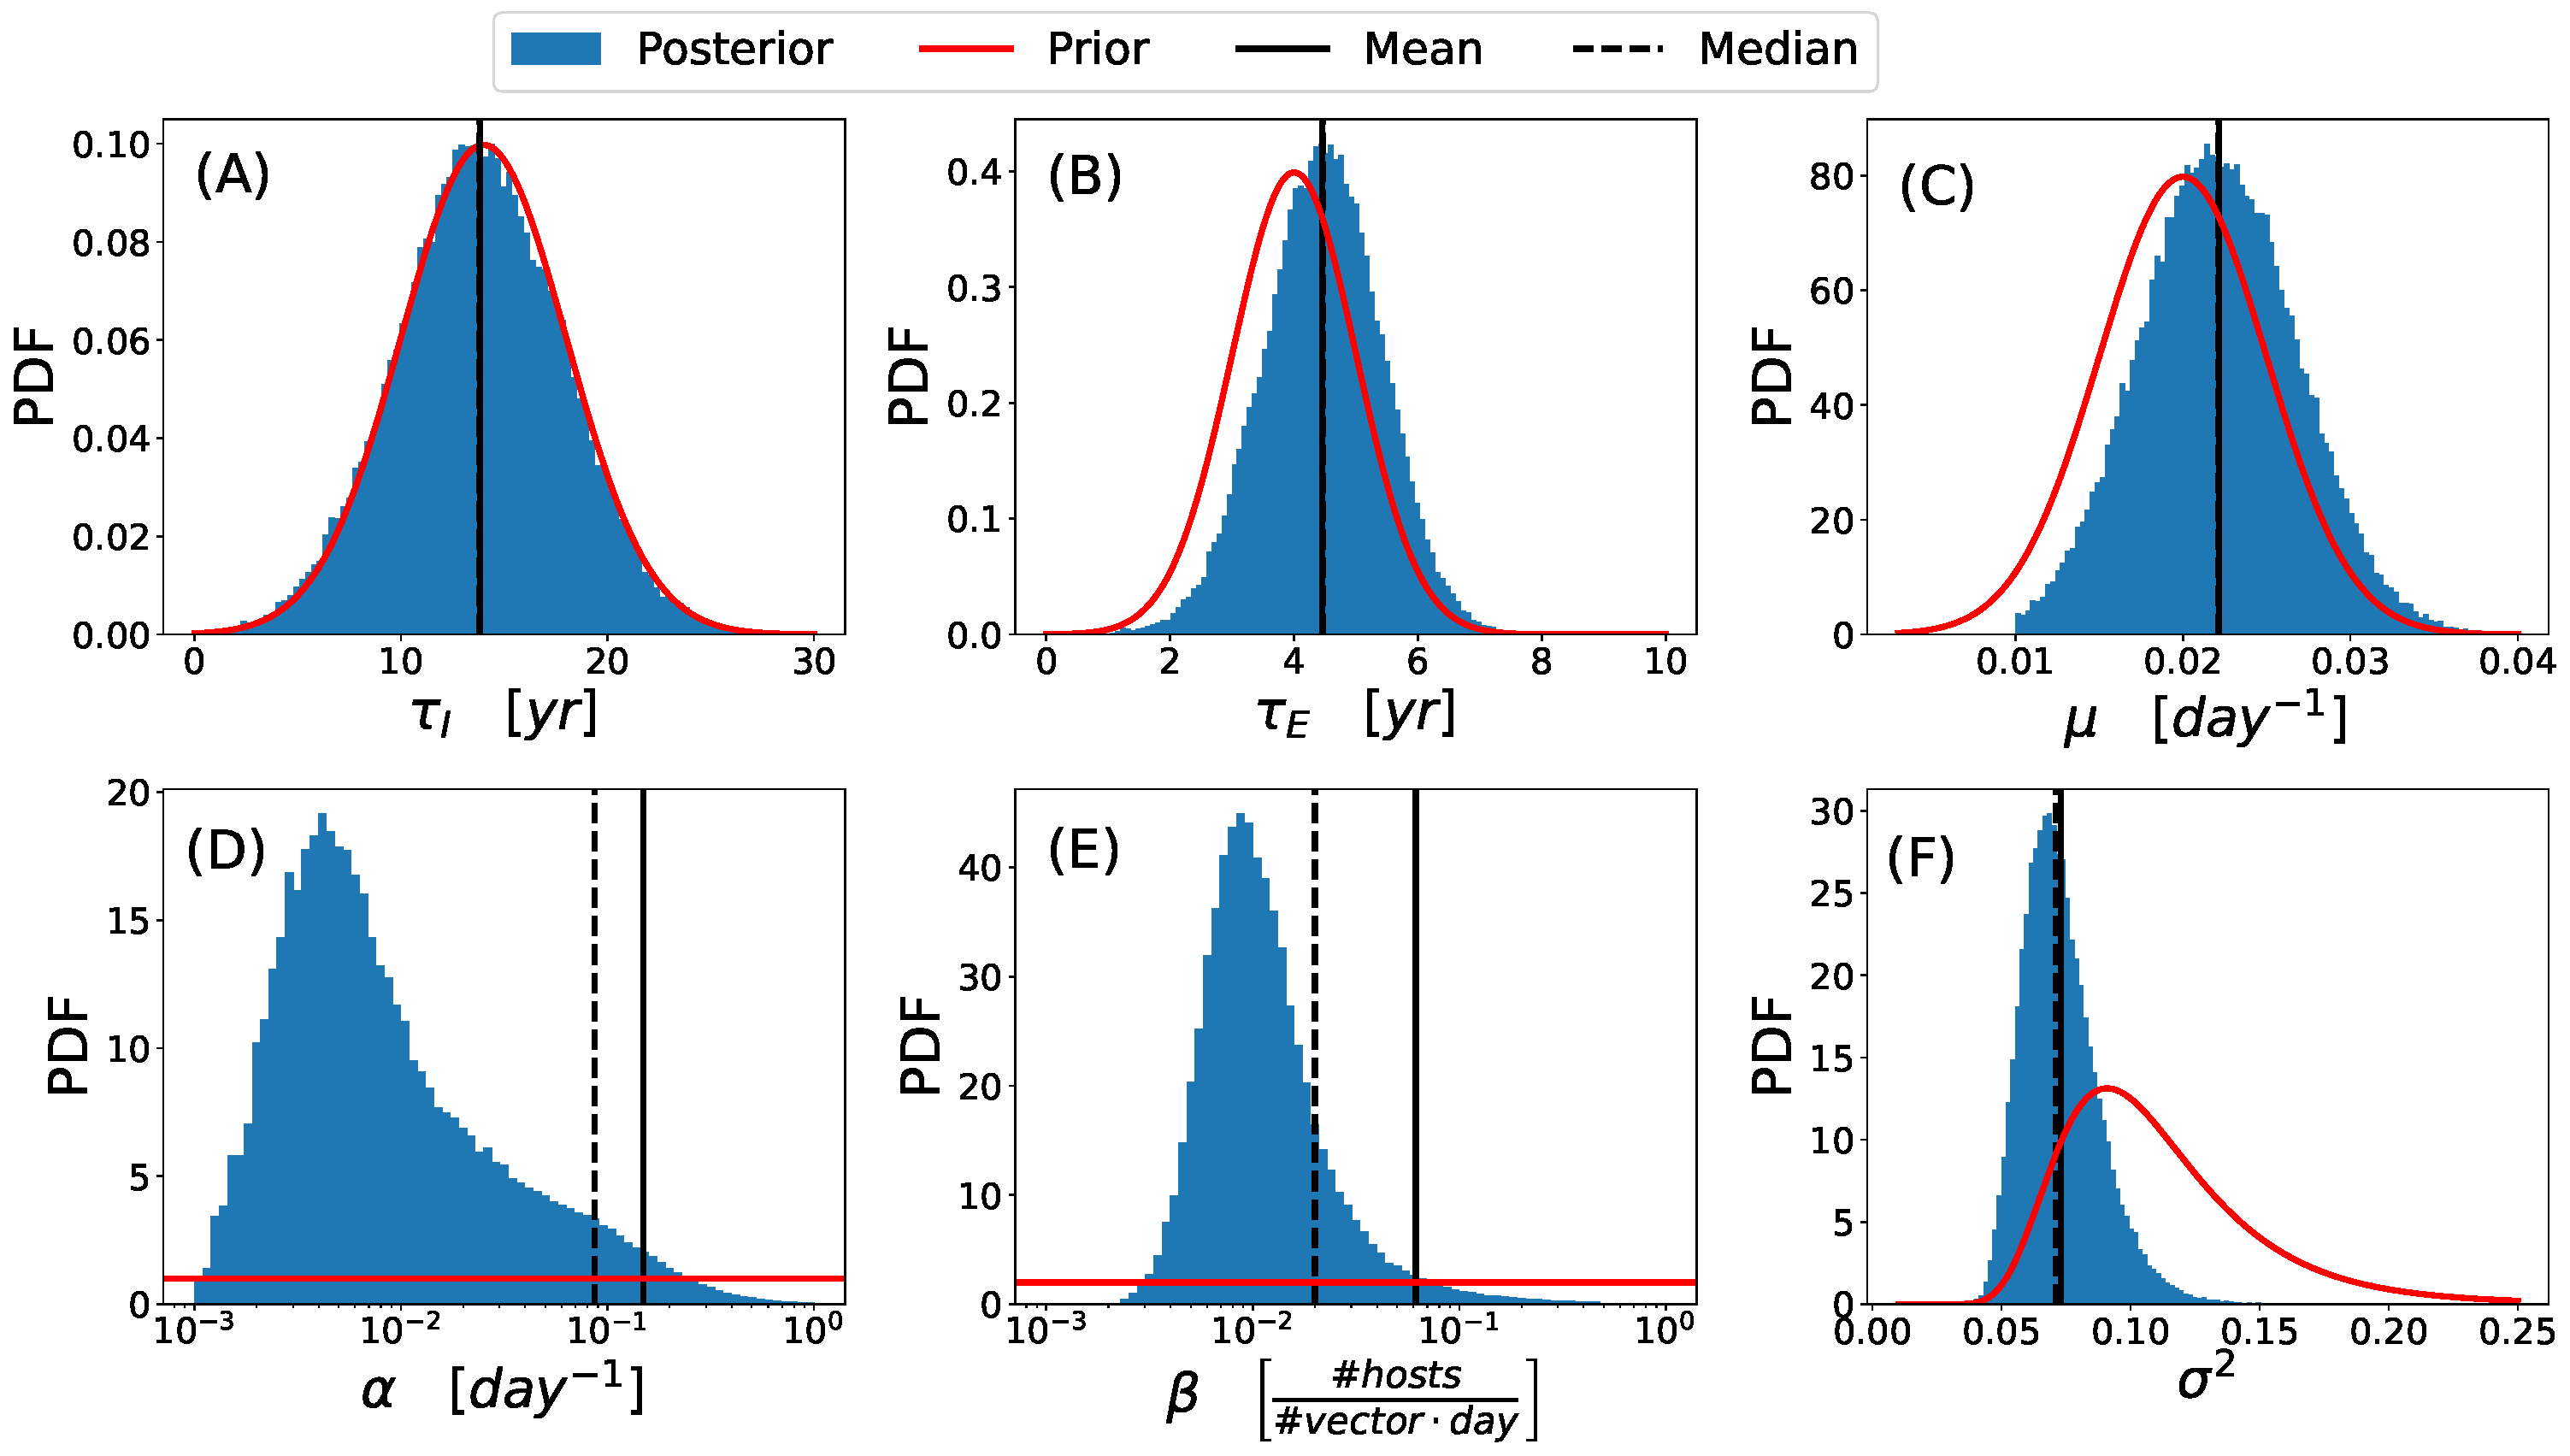
\includegraphics[width=0.9\textwidth]{Figures/Parameter_estimates_ALSD.pdf}
    \caption[Posterior and prior distributions of the model parameters for
        ALSD]{Posterior (blue histograms) and prior (red line) distributions
        of the model parameters for ALSD. Solid and dashed black lines
        correspond to
        the mean and median of the posterior distributions. (A) Host infectious
        period
        $\tau_I=1/\gamma$. (B) Host latent period $\tau_E=1/\kappa$.  (C)
        Vector
        removal rate $\mu$. (D) Vector infection rate $\alpha$. (E) Host
        infection rate
        $\beta$. (F) The variance of the field data $\sigma^2$.}
    \label{fig:parameter_estimates_ALSD}
\end{figure}

\begin{figure}[H]
    \centering
    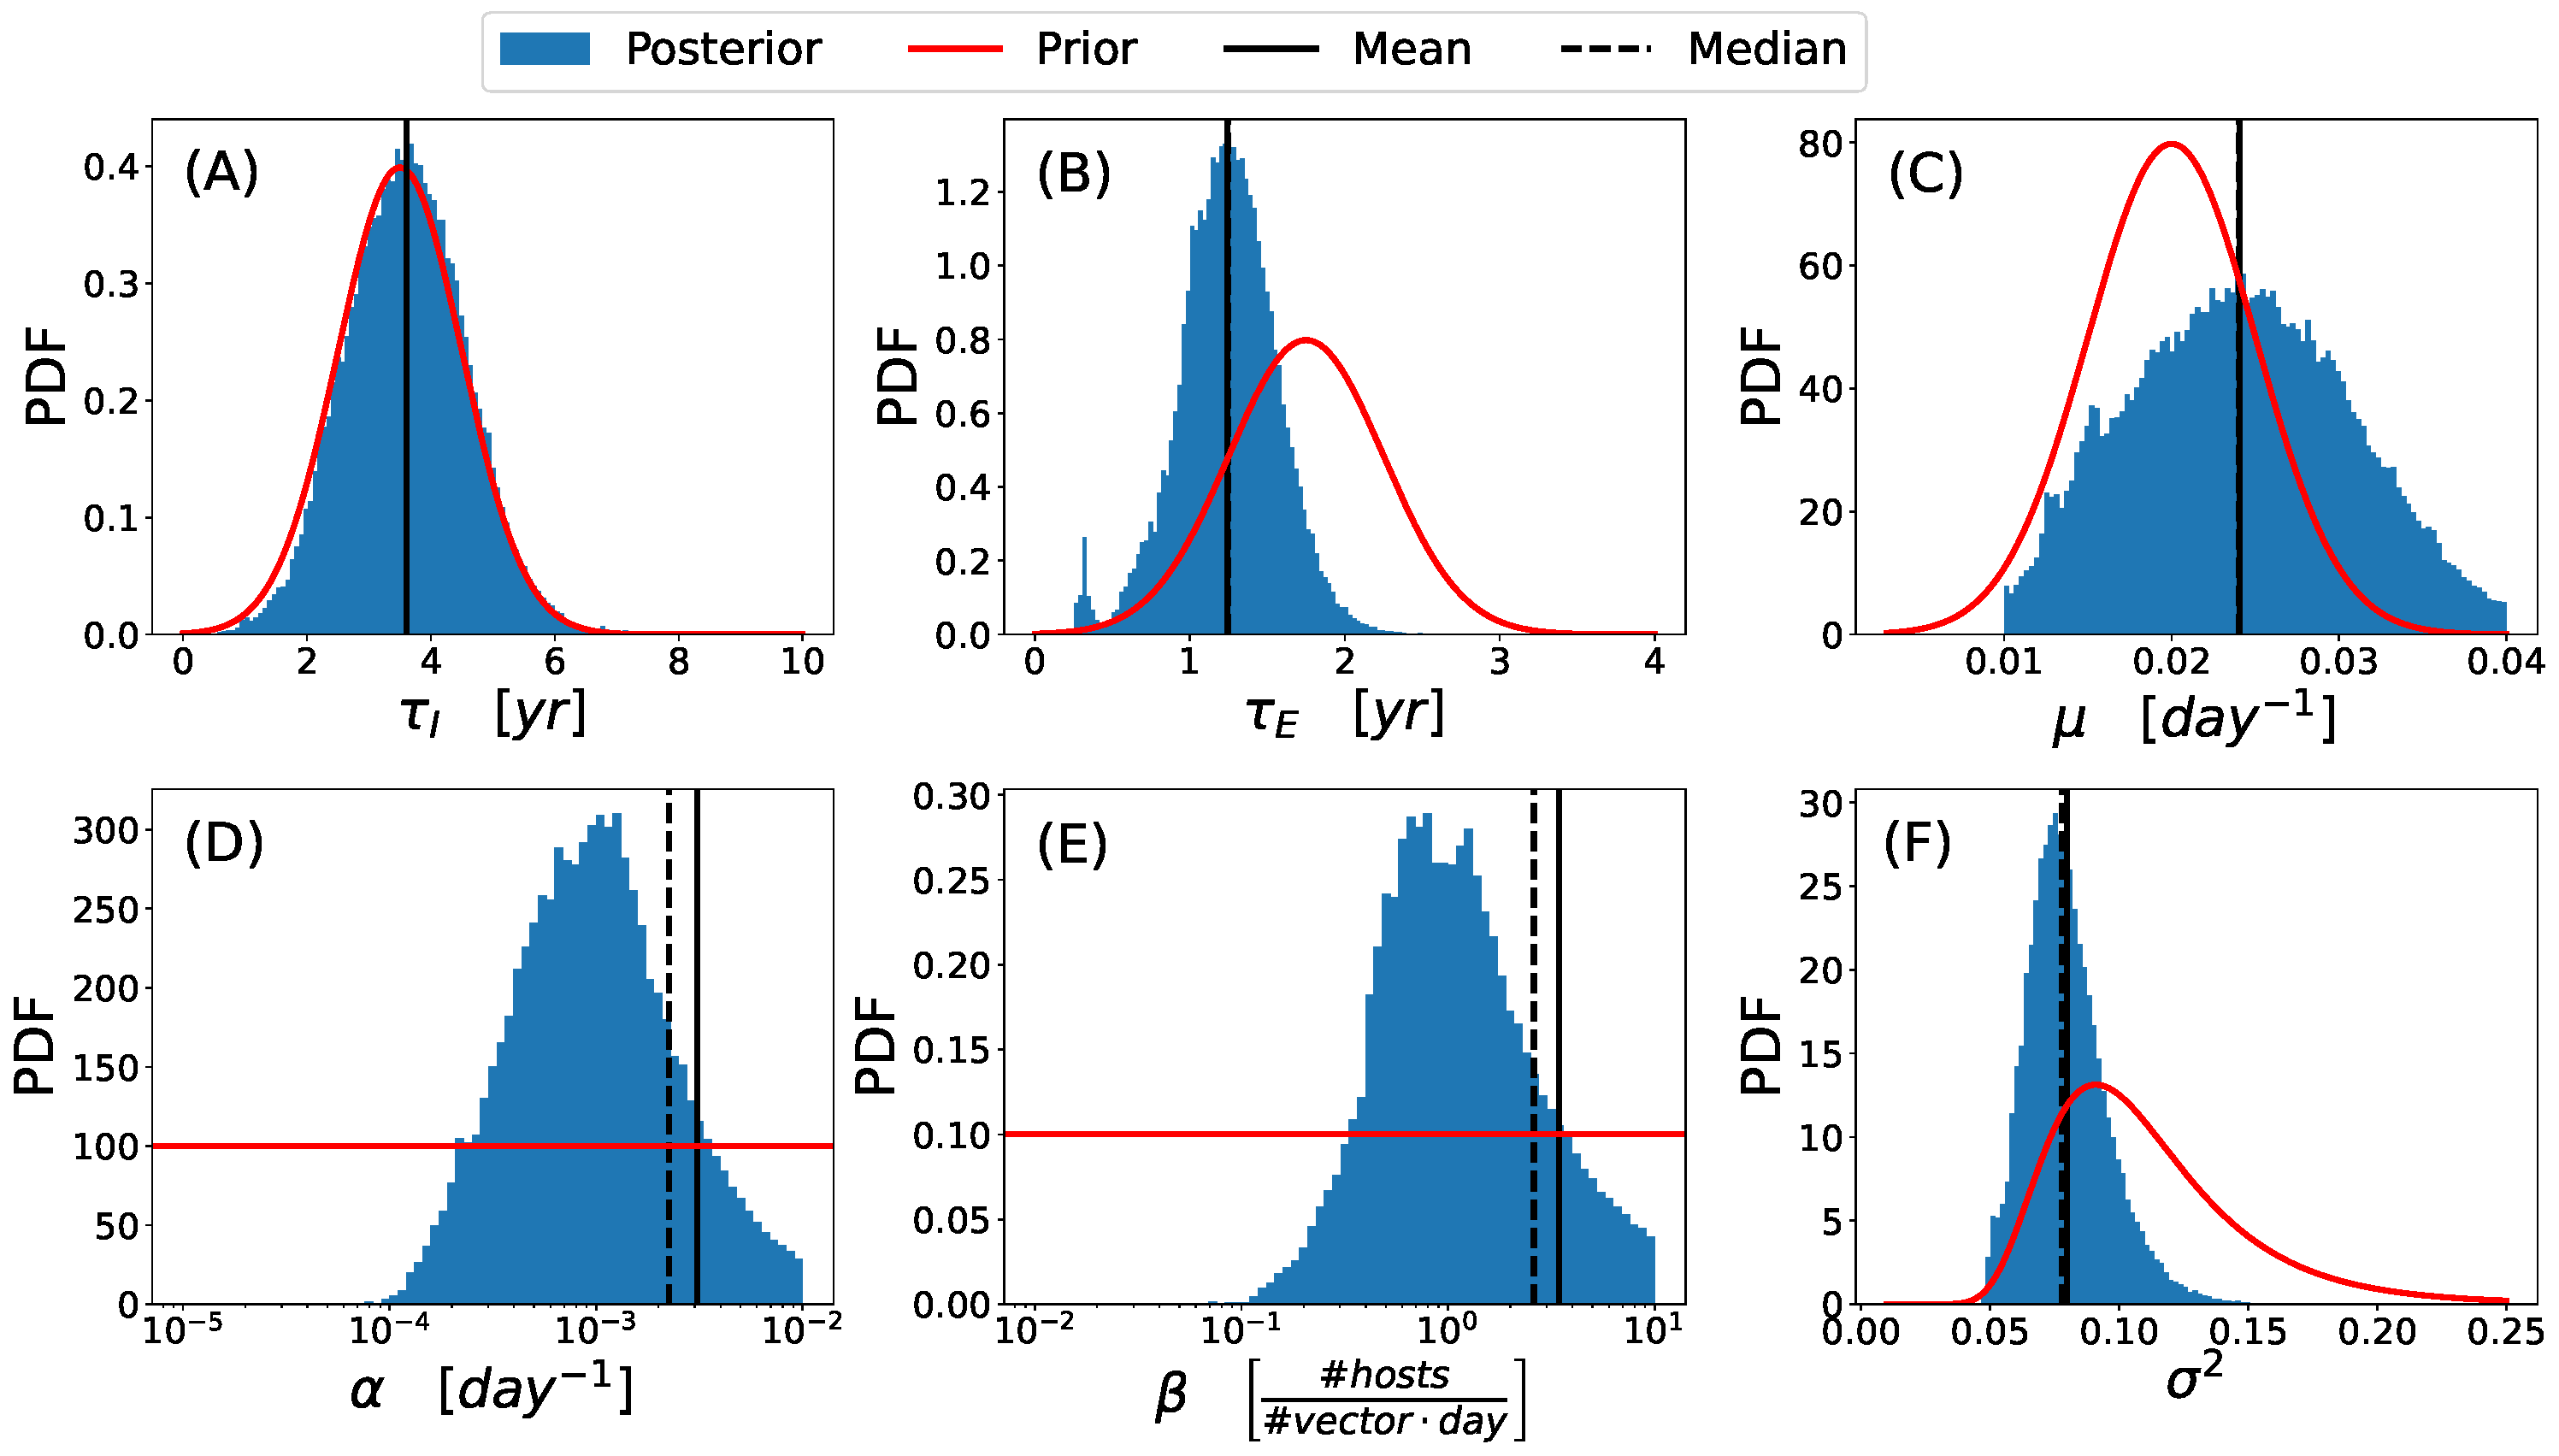
\includegraphics[width=0.9\textwidth]{Figures/Parameter_estimates_OQDS.pdf}
    \caption[Posterior and prior distributions of the model parameters for
        OQDS]{Posterior (blue histograms) and prior (red line) distributions
        of the model parameters for OQDS. Solid and dashed black lines
        correspond to
        the mean and median of the posterior distributions. (A) Host infectious
        period
        $\tau_I=1/\gamma$. (B) Host latent period $\tau_E=1/\kappa$. (C) Vector
        removal
        rate $\mu$. (D) Vector infection rate $\alpha$. (E) Host infection rate
        $\beta$. (F) Variance of the field data $\sigma^2$.}
    \label{fig:parameter_estimates_OQDS}
\end{figure}

Mean and median parameter estimates, i.e. the best-fit parameter values for
ALSD and OQDS, are summarized in
\cref{tab:parameter_estimates_ALSD,tab:parameter_estimates_OQDS}, respectively.
As already seen from the posterior distributions, the best-fit values for
$\tau_E$, $\tau_I$ and $\mu$ are close to the ones given by literature and
field data for both diseases. Conversely, $\alpha$ and $\beta$ are rather
uninformative, as their 95\% confidence intervals cover almost two orders of
magnitude. This again indicates that without some data about the evolution of
the vector states in time, $S_v(t)$ and $I_v(t)$, it is nearly impossible to
derive the proper values for these parameters.

\begin{table}[H]
    \centering
    \caption[Estimated parameters of the model for ALSD in Mallorca]{Estimated
        epidemiological
        parameters from Bayesian model
        fitting to the disease progression curve of ALSD in Mallorca.}
    \resizebox{\textwidth}{!}{
        \begin{tabular}{cccccc}
            \hline \hline
            \textbf{Parameter}      & \textbf{Definition}       &
            \textbf{Units}          &
            \textbf{Posterior Mean} & \textbf{Posterior Median} & \textbf{95\%
                C.I.}
            \\
            \hline
            $\tau_I$                & Host infectious period    & yr
                                    & $13.84$                   & $13.82$
                                    &
            $[7.12, 20.47]$
            \\
            $\tau_E$                & Host latent period        & yr
                                    & $4.46$                    & $4.47$
                                    & $[2.88,
                        5.99]$
            \\
            $\beta$                 & Host infection rate       &
            $\SI{}{\frac{\#host}{\#vector
            \cdot day}}$            & $0.062$                   & $0.02$
                                    & $[0.0061, 0.3013]$
            \\
            $\alpha$                & Vector infection rate     &
            $\SI{}{day^{-1}}$       & $0.15$                    &
            $0.086$                 & $[0.0047, 0.54]$
            \\
            $\mu$                   & Vector removal rate       &
            $\SI{}{day^{-1}}$       & $0.0222$                  &
            $0.0221$                & $[0.015, 0.030]$
            \\
            $R_0$                   & Basic reproductive number & -
                                    & 133                       & 25
                                    & -
            \\ \hline
            \hline
        \end{tabular}
    }
    \label{tab:parameter_estimates_ALSD}
\end{table}

\begin{table}[H]
    \centering
    \caption[Estimated parameters of the model for OQDS in Apulia]{Estimated
        epidemiological parameters from Bayesian model
        fitting to the disease progression curve of OQDS in Apulia.}
    \resizebox{\textwidth}{!}{%
        \begin{tabular}{cccccc}
            \hline \hline
            \textbf{Parameter}      & \textbf{Definition}       &
            \textbf{Units}          &
            \textbf{Posterior Mean} & \textbf{Posterior Median} & \textbf{95\%
                C.I.}
            \\
            \hline
            $\tau_I$                & Host infectious period    & yr
                                    & $3.61$                    & $3.60$
                                    & $[2.06,
                        5.20]$
            \\
            $\tau_E$                & Host latent period        & yr
                                    & $1.24$                    & $1.25$
                                    & $[0.70,
                        1.75]$
            \\
            $\beta$                 & Host infection rate       &
            $\SI{}{\frac{\#host}{\#vector
            \cdot day}}$            & $3.44$                    & $2.60$
                                    & $[0.55, 8.79]$
            \\
            $\alpha$                & Vector infection rate     &
            $\SI{}{day^{-1}}$       & $0.0031$                  &
            $0.0022$                & $[0.0005, 0.0084]$
            \\
            $\mu$                   & Vector removal rate       &
            $\SI{}{day^{-1}}$       & $0.0240$                  &
            $0.0240$                & $[0.014, 0.035]$
            \\
            $R_0$                   & Basic reproductive number & -
                                    & 33                        & 21
                                    & -
            \\ \hline
            \hline
        \end{tabular}
    }
    \label{tab:parameter_estimates_OQDS}
\end{table}

Overall, the data falls within the 99\% confidence limits of the fitted
model for both the ALSD and OQDS outbreaks (\cref{fig:best_fit_model} (B,D)).
We
also computed the instantaneous reproductive number, $R_0(t)$, by using
\cref{eq:R0} with $S_H(t)$ instead of only $S_H(0)$ along the simulation.
Noteworthy, $R_0(t)=1$ coincides with the stopping of new infections being
produced, i.e. the number of exposed hosts does not increase
(\cref{fig:best_fit_model} (A,C)). This supports our approximate method for
computing the reproductive number for Xf diseases (\cref{app:R0},
\cref{eq:R0}). Due to the different time scales of both epidemics
($\tau_I^{ALSD}+\tau_E^{ALSD} > \tau_I^{OQDS}+\tau_E^{OQDS}$), the OQDS
outbreak dies out earlier than the one for ALSD.

We notice that for ALSD a large proportion of the vector population gets
infected every year (\cref{fig:best_fit_model} (A)), while a very small
proportion is needed in OQDS to produce a lethal outbreak
(\cref{fig:best_fit_model} (C)). However, this last statement is rather
unrealistic, as around 50\% of the vectors that are captured in Apulia are
indeed infected by Xf \cite{Cavalieri2019,cornara2017transmission}. Thus, the
evolution of the infected vector population should be qualitatively similar to
that obtained for ALSD (\cref{fig:best_fit_model} (C)). As previously
explained,
different suitable combinations of $\alpha$ and $\beta$ parameters should give
rise to similar progression curves for the hosts while different ones for the
vectors, but the realistic values for these parameters cannot be obtained from
the Bayesian fit due to the lack of data of the vector states, $S_v(t)$,
$I_v(t)$.

\begin{figure}[H]
    \centering
    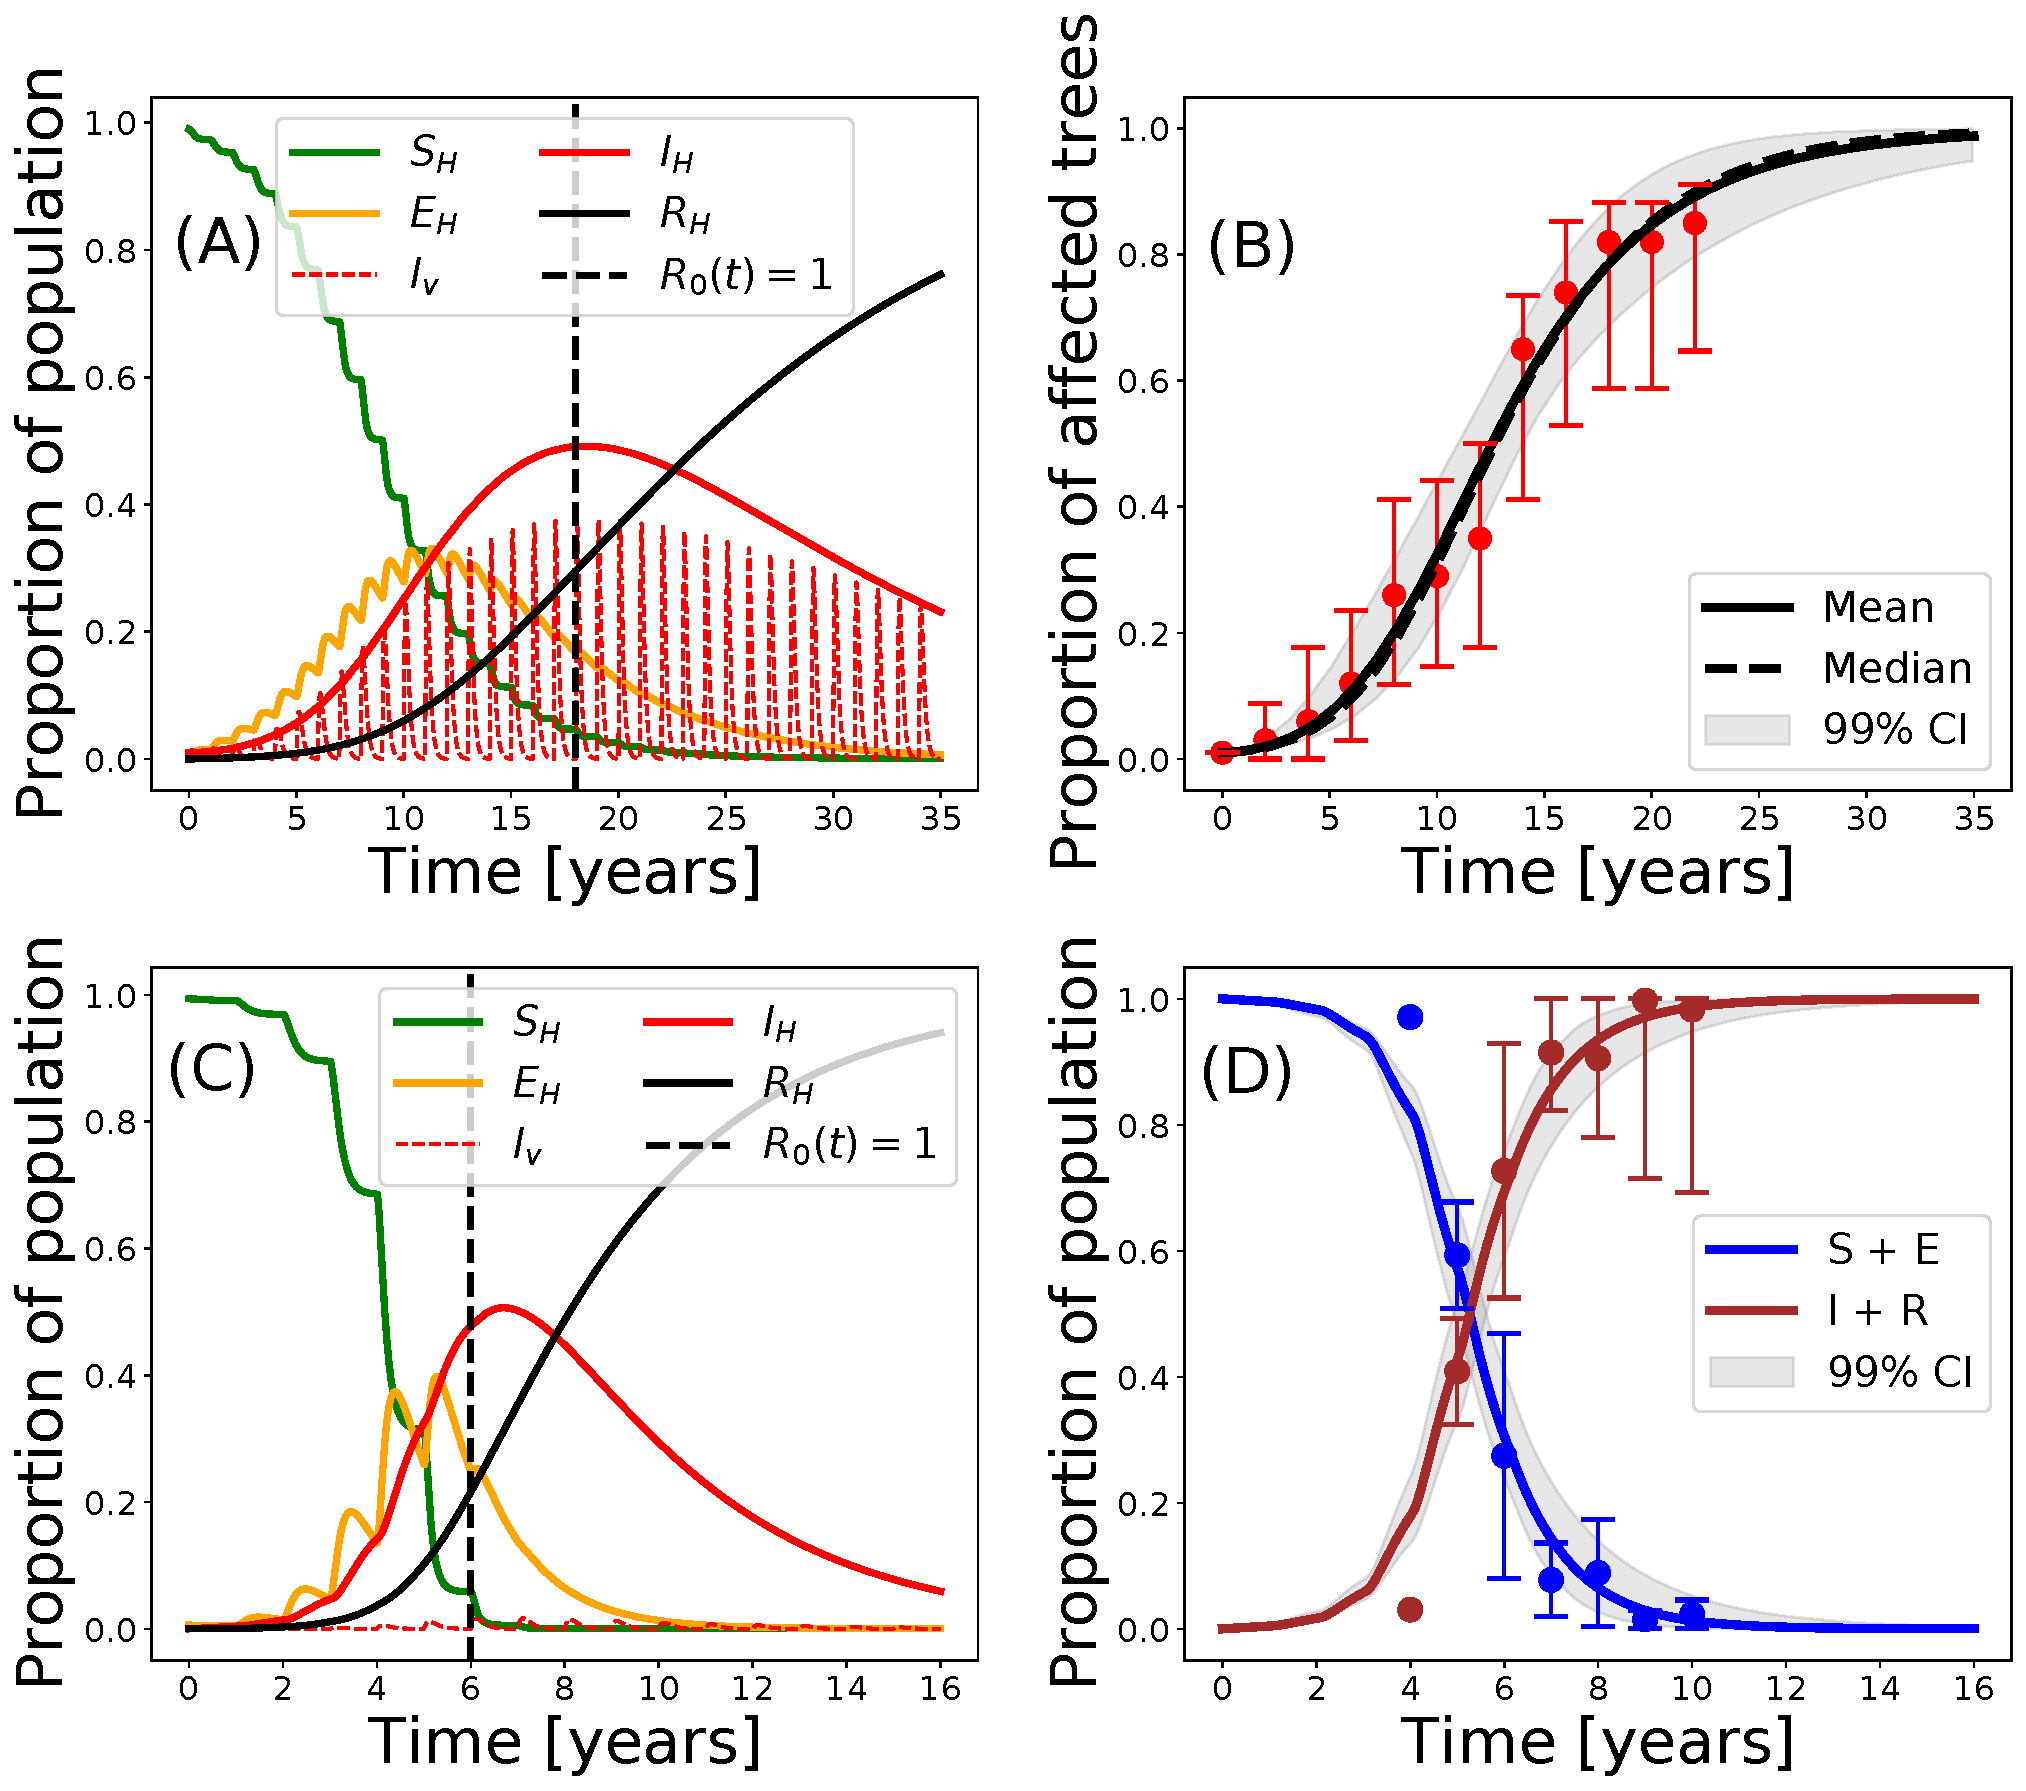
\includegraphics[width=0.9\textwidth]{Figures/BayesianInference.pdf}
    \caption[Best-fit model to the field data for ALSD and OQDS]{(A) Simulation
        of the model with the best-fit parameters for
        ALSD. (B) Model fit to field data by means of the mean and median
        values of the
        posterior distributions of the parameters for ALSD. (C) Simulation of
        the model
        with the best-fit parameters for OQDS. (D) Model fit to field data by
        means of
        the mean and median values of the posterior distributions of the
        parameters for
        OQDS. The gray-shaded area corresponds to the 99\% confidence interval.
        The
        error bars for the field data correspond to their 95\% confidence
        interval
        obtained with a bootstrapping technique.}
    \label{fig:best_fit_model}
\end{figure}

Nevertheless, by manually exploring other values for $\alpha$ and $\beta$
parameters, we can obtain a more biologically plausible scenario for the OQDS
that is still able to fit the available data for the hosts.
\cref{fig:best_fit_model_OQDS} (A) shows a simulation of the model with
previously inferred best-fit median parameters for OQDS. By changing the values
of $\alpha$ and $\beta$, we obtain a more realistic scenario, i.e. around a
50\% of the vector population getting infected during the outbreak
(\cref{fig:best_fit_model_OQDS} (B)) \cite{Cavalieri2019,
    cornara2017transmission}. Noteworthy, the $\beta$ value obtained in this
way
is almost identical to the transmission rate recently reported by
\cite{Bodino2021} for OQDS. This change in the transmission parameters only
affects the progression curve of the infected vector population, being the
progression of the host compartments practically unchanged
(\cref{fig:best_fit_model_OQDS} (C)). Anyway, both sets of parameter values for
$\alpha$ and $\beta$ can properly fit the field data, corresponding exclusively
to the	host population (\cref{fig:best_fit_model_OQDS} (D)).

The model adjusted to the progression curves of both diseases indicates
that the transmission rate $\alpha$ must be greater than $\beta$ when the
proportion of infected vectors is relatively high ($>30\%$). We checked if the
relation between $\alpha$ and $\beta$ held when changing the assumed
$N_v(0)=N_H/2$, obtaining that it kept approximately the same for very
different values of the initial vector population.

\begin{figure}[H]
    \centering

    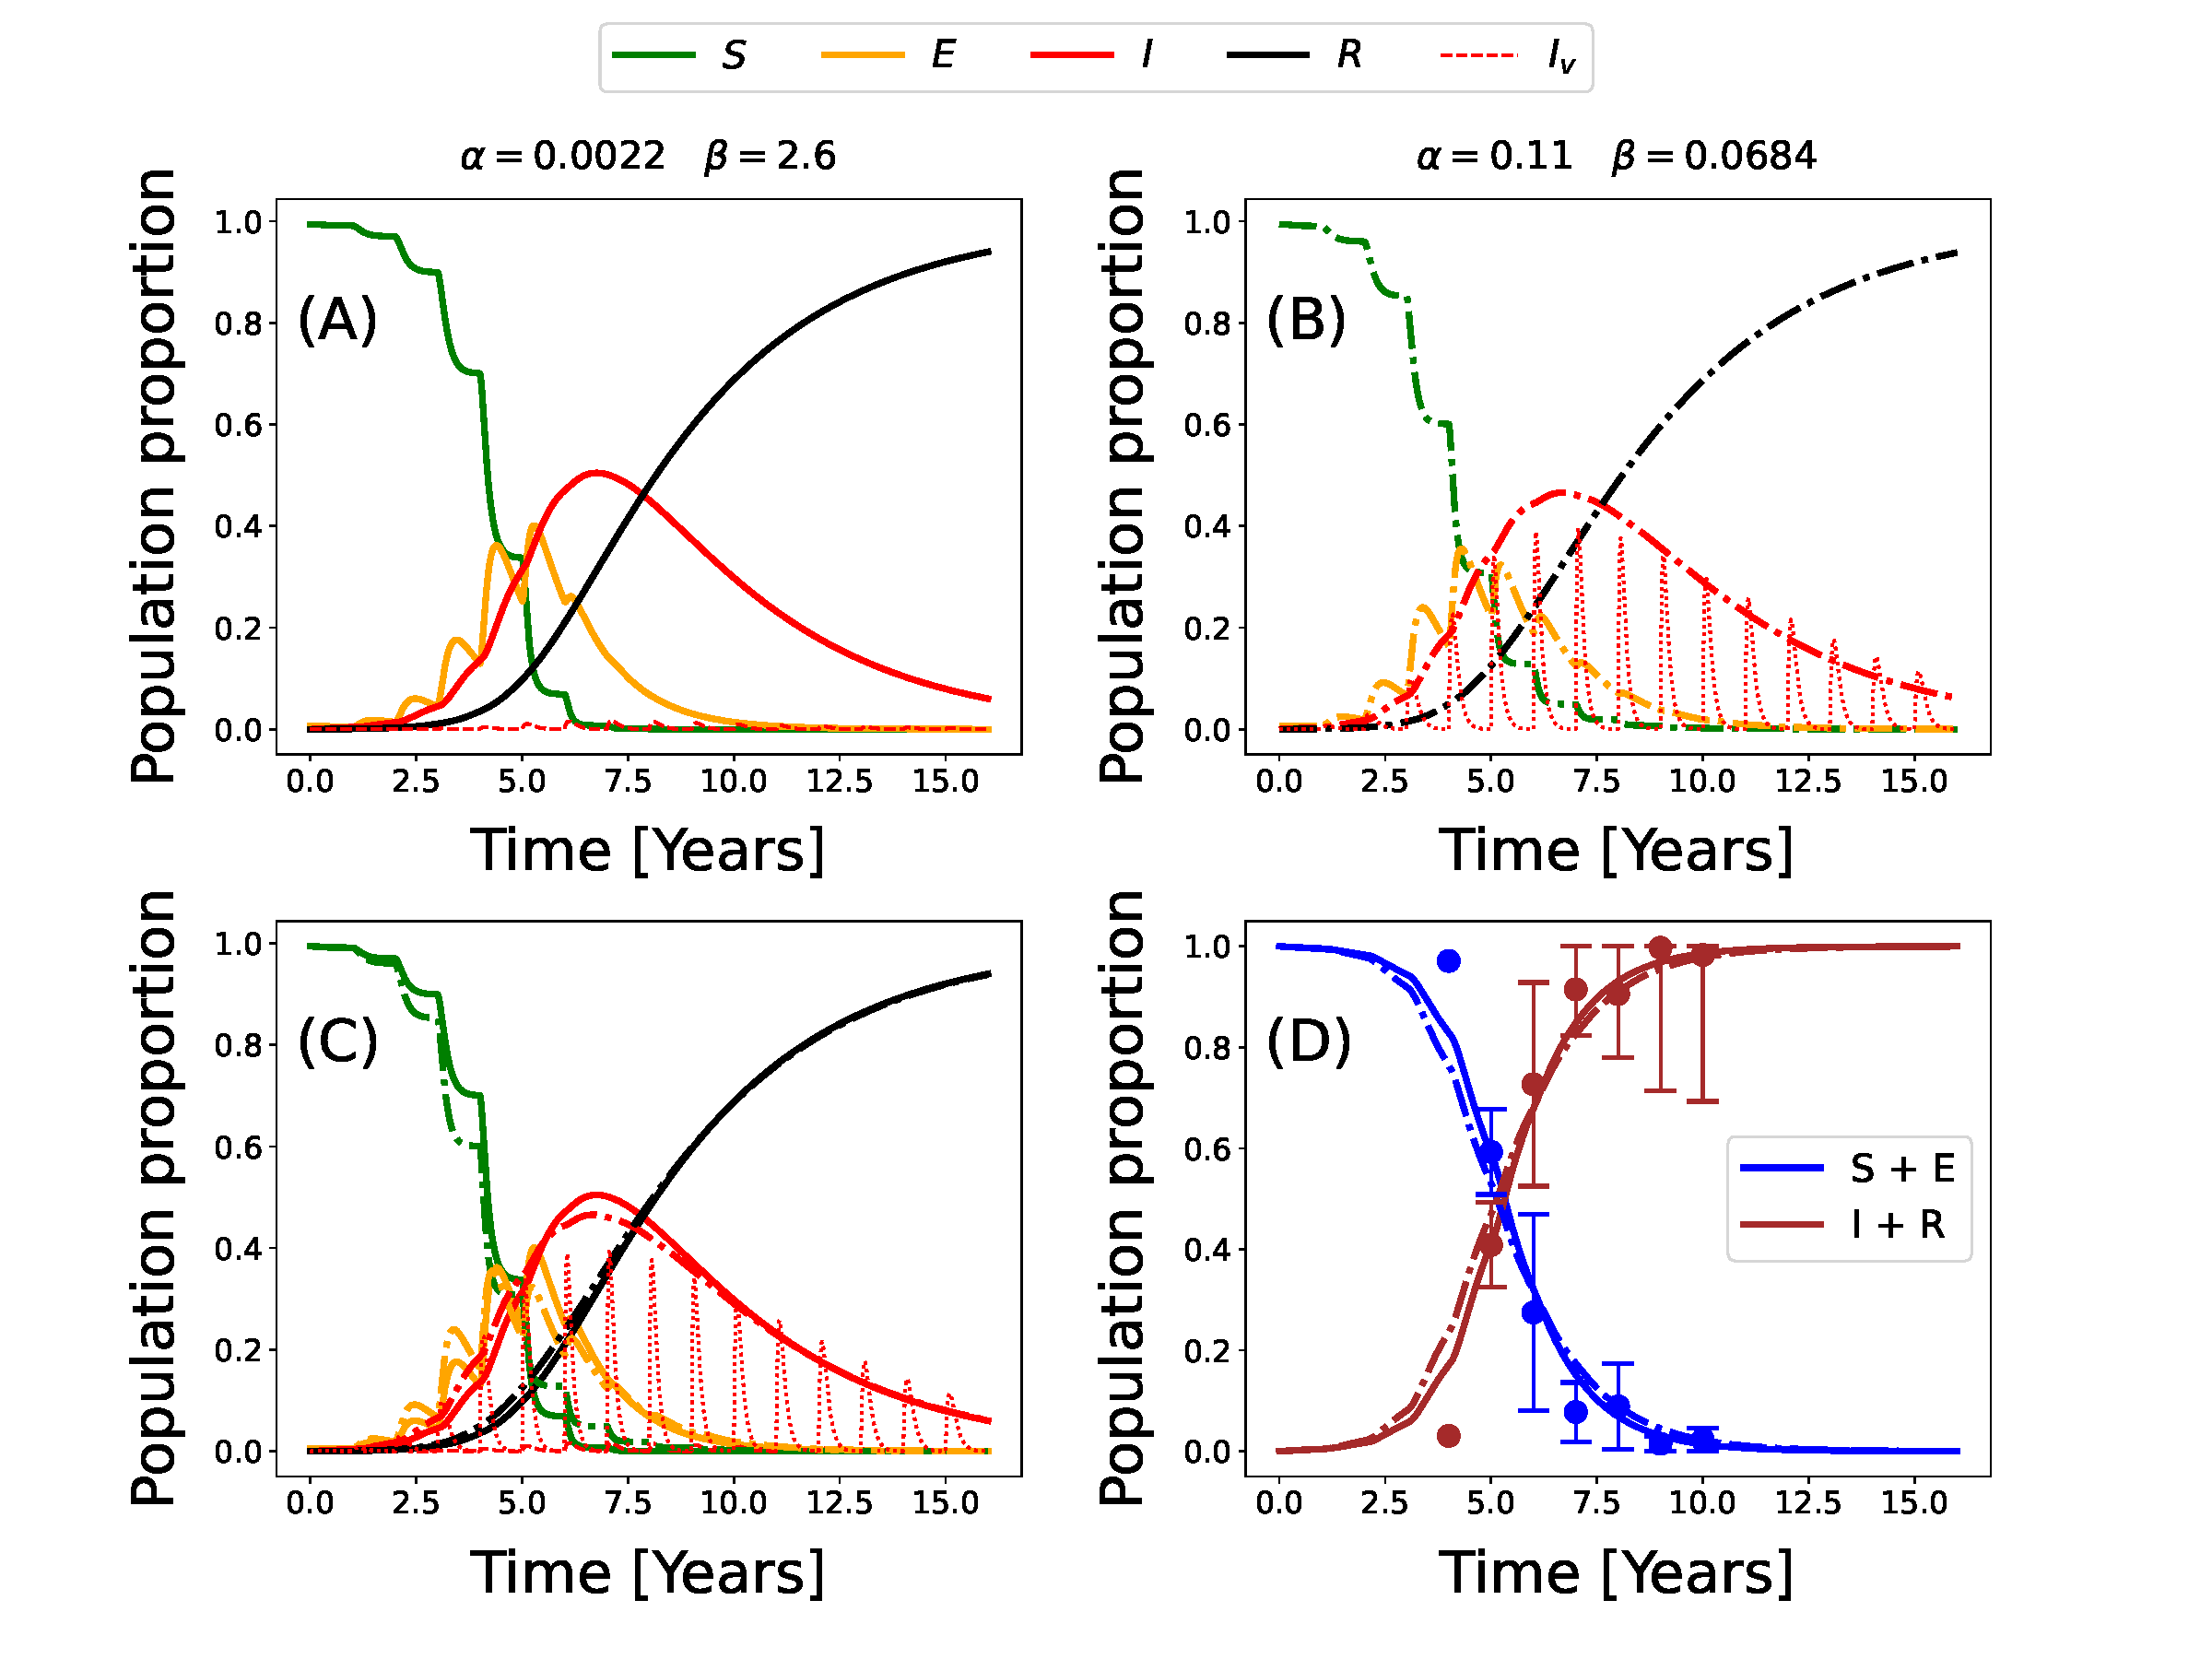
\includegraphics[width=\textwidth]{Figures/OQDS_different_vector_curves_same_host_curve.pdf}
    \caption[Comparison of the model fit to the data for OQDS with different
        transmission rates]{(A) Simulation of the model with the original
        best-fit
        parameters for OQDS. (B) Simulation of the model with the original
        best-fit
        parameters for OQDS but with different $\alpha$, $\beta$ values. (C)
        Comparison
        of the progression curves. Note that the curves for the hosts are very
        similar
        while the curve for the infected vector population is very different.
        (D)
        Comparison of the model fit to the data with both simulations. Solid
        lines
        correspond to results with the original best-fit parameters while
        dash-dot
        lines correspond to the results of the more realistic scenario with
        different
        $\alpha$ and $\beta$.}
    \label{fig:best_fit_model_OQDS}
\end{figure}

\subsection{Global Sensitivity Analysis}

We computed the sensitivity indices for the model parameters with respect
to the more relevant quantities of interest, namely, the time at which the
number of infectious hosts is maximal, $t_{\textrm{peak}}$, the maximum number
of infectious hosts, $I_{\textrm{peak}}$ and the final number of dead hosts,
$R_\infty$. The results were obtained exploring the parameter space constrained
to the intervals $\{\beta\in(0.001, 0.1), \ \tau_E\in(3,7), \ \tau_I\in(5,25),
    \ \alpha\in(0.001, 1), \ \mu\in(0.01, 0.04)\}$ using $10^4$ Quasi-Monte
Carlo
samples and are summarized in \cref{fig:GSA}.

Parameters $\alpha, \ \beta$ and $\mu$ are the most influential with regard
to the time at which the infectious host population peaks, $t_{peak}$, the
magnitude of the peak, $I_{peak}$, and the final number of dead hosts,
$R_{\infty}$. The total output variance (total order indices) cannot be
explained by the variances of the parameters alone (first order indices)
(\cref{fig:GSA}). Therefore, higher-order interactions among the parameters
importantly affect the sensitivity of the quantities under study. Indeed, the
contribution to the total output variance of $\gamma$ and $\kappa$ for
$t_{peak}$ and $R_{\infty}$ come notably from higher-order interactions. This
can be checked in panels (B,C,F) of \cref{fig:GSA}, in which the contribution
to the output variance from interactions between pairs of parameters (second
order indices) is represented. Interactions among the parameters contribute to
increasing the output variance with respect to $t_{peak}$ and $I_{peak}$, while
the effect is more heterogeneous in the case of $R_{\infty}$. In particular,
the interactions between $\alpha-\beta$ and $\alpha-\mu$ produce the main
contributions to the increase of output variance in all cases, while
$\kappa-\beta$, $\kappa-\alpha$ and $\kappa-\mu$ interactions decrease the
output variance.

\begin{figure}[H]
    \centering
    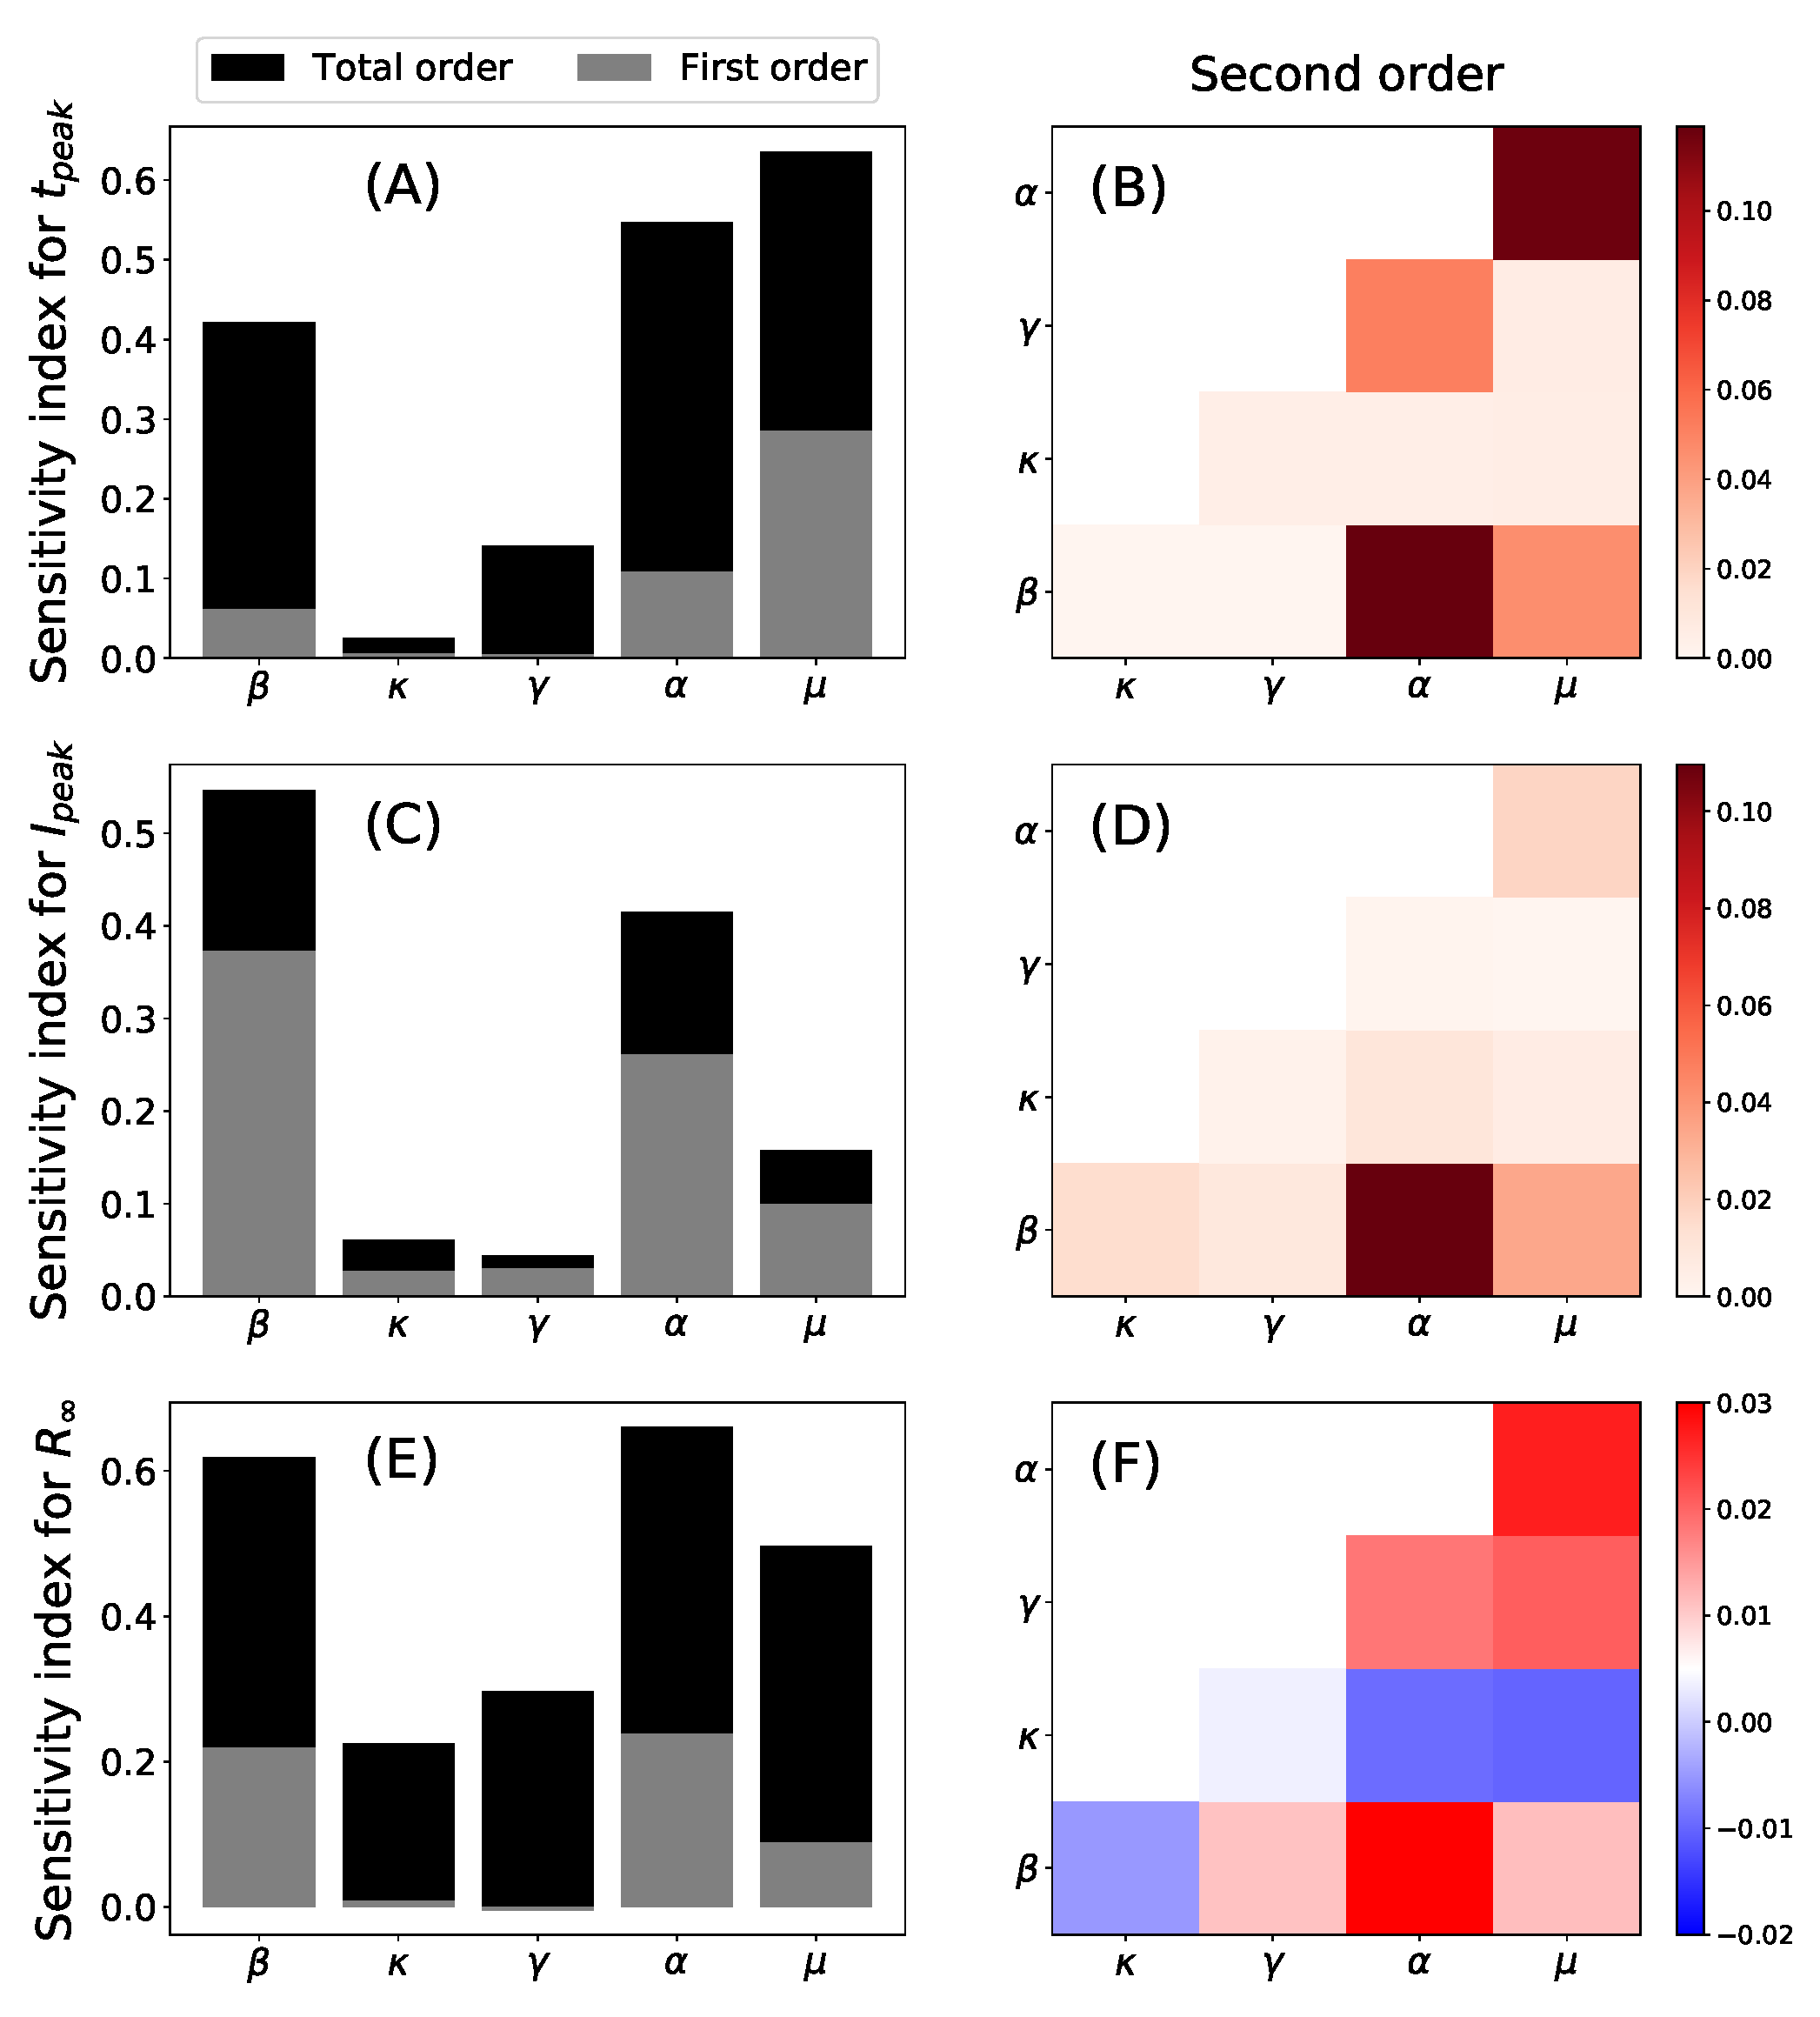
\includegraphics[width=0.75\textwidth]{Figures/GSA.pdf}
    \caption[Global Sensitivity Analysis of the model]{Global Sensitivity
        Analysis of the model parameters performed
        with the Sobol method with respect to the time at which the infectious
        population peaks, $t_{peak}$ (A-B), the magnitude of this peak,
        $I_{peak}$
        (C-D) and the final number of dead hosts, $R_{\infty}$ (E-F). The left
        column
        (A,C,E) shows the total and first-order indices and the right column
        (B,D,F)
        shows the second-order indices.}
    \label{fig:GSA}
\end{figure}

\subsection{Epidemic control through vector management}

The sensitivity analysis clearly indicates that acting on $\alpha,\beta$
and $\mu$ is the best strategy to lower disease incidence and mortality.
However, controlling transmission rates is cumbersome so a different control
strategy based only on vector control is considered in this section. In our
model, there are two ways of implementing vector-population control: (i)
decreasing the typical time, $1/\mu$, that vectors spend between crops each
year by some mechanism (thus increasing $\mu$) and (ii) reducing the initial
number of vectors that invade crops each year (e.g. lowering $N_v(0)$ via egg
or nymph control \cite{Lago2022}).

We analyzed the effect of vector management by simulating epidemic
outbreaks using different values of $\mu$ and $N_v(0)$, and keeping the rest of
parameters as fitted for both ALSD and OQDS outbreaks
(\cref{fig:control_strategy}). In both epidemics, decreasing the presence time
as well as the number of vectors contribute to controlling the epidemic by
lowering $R_0$ and, consequently, the final size of the epidemic, $R_{\infty}$.
Furthermore, we observe that decreasing vector presence is more efficient than
decreasing its annual initial population, i.e. we further reduce $R_{\infty}$,
the final size of the epidemic, by applying a similar reduction in the
residence time $1/\mu$. This could also be anticipated as $R_0$ depends
quadratically on $1/\mu$ while only linearly on $N_v(0)$ (\cref{eq:R0}).
However, the minimal intervention strategy, starting from the current situation
in the $(1/\tau,N_v(0))$ parameter space that yields an absolute control of the
epidemic, $R_0<1$, involves a mixed strategy of lowering both $1/\mu$ and
$N_v(0)$.

\begin{figure}[H]
    \centering
    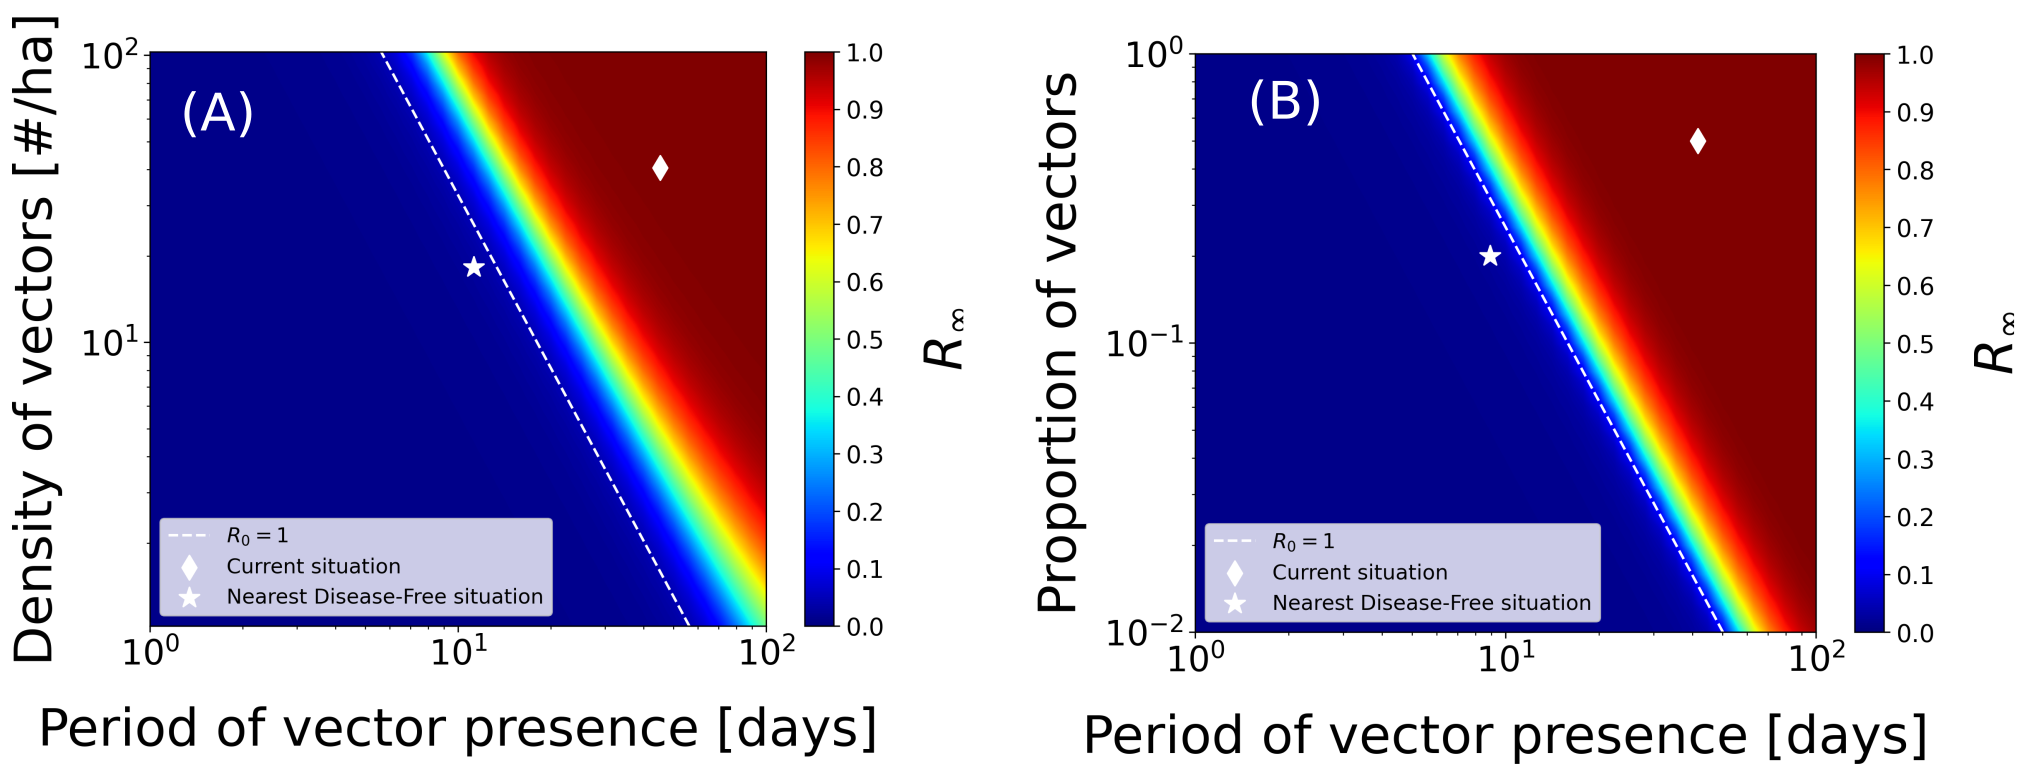
\includegraphics[width=\textwidth]{Figures/Control_strategy.png}
    \caption[Epidemic control through vector management for ALSD in Mallorca
        and
        OQDS in Apulia]{Epidemic control through vector management for ALSD in
        Mallorca (A) and OQDS in Apulia (B). The white shaded line denotes
        $R_0=1$, the
        white diamond corresponds to the parameter values of the fitted model.
        The
        white star is the closest disease-free state to the current situation
        in this
        representation.}
    \label{fig:control_strategy}
\end{figure}

\section{Discussion}

In this work, we have developed a deterministic continuous-time
compartmental model for \textit{Xylella fastidiosa} vector-borne diseases in
Europe. The model attempts to characterize the main biotic processes that lead
to the development of epidemics, including the seasonal dynamics of the main
vector, \textit{P. spumarius}. We show how the model is sufficiently general to
represent with some accuracy the parameters that determine the ALSD in Mallorca
(Spain) and the OQDS in Apulia (Italy), both transmitted by \textit{P.
    spumarius}. To our best knowledge, this is the first mathematical model
describing Xf epidemics that considers the temporal pattern of vector abundance
observed in field data, faithfully representing the known biological
information about the pathosystem. It includes a dynamic approximation of the
non-stationary populations of \textit{P. spumarius}, mathematically represented
by a sporadic source term through which vectors are born every year, and an
exponential decay term. Due to the non-stationarity of the vector dynamics,
$R_0$ in the model cannot be computed with standard methods such as the Next
Generation Matrix \cite{Diekmann2010}. To circumvent this problem, we applied
an approximate method to compute it as previously proposed by
\cite{GimenezRomero2022_PRE}. We show that this approximate $R_0$ correctly
characterizes the epidemic, further validating the method proposed by
\cite{GimenezRomero2022_PRE}.

Nonlinear mathematical models of disease transmission enhance our
understanding of the different mechanisms operating in an epidemic, especially
compared with correlative or machine learning methods, often very useful in
practice but offering very little understanding. A key aspect to render these
models useful is the determination of the parameters from available data. If
this step can be properly performed, these models become very predictive and
especially helpful to design disease control strategies. However, an
appropriate calibration of the model relies on access to good-quality field
data, which is often the bottleneck for the application of this kind of models.
In the present study, the parameters have been obtained using a Bayesian
inference framework, which relies on probability distributions rather than
point-like measures. This way, mean or median values can be considered together
with their confidence intervals able to characterize the robustness of the
obtained parameters. In general, we obtained different values of the parameters
for the ALSD and OQDS outbreaks in Mallorca and Apulia, respectively. The
fitted values, however, are in good agreement with previous field-based
measures for each disease while the differences observed between both outbreaks
may reflect differences between the Xf subspecies and crops involved (deciduous
vs. evergreen).

One of the conclusions of the study is that the available data for both
diseases is not enough to obtain robust estimates for all of the model
parameters. The lack of data about the vector population compartments yields
many possible values for the parameters that regulate transmission, $\alpha$
and $\beta$, provided that the progression of the host compartments correctly
fits the field data. In other words, very infectious vectors (high $\beta$)
that hardly ever get infected (low $\alpha$) can produce a similar outbreak
within the host population to that produced by very low infectious vectors (low
$\beta$) that get infected very often (high $\alpha$). The great difference in
these situations would be that, in the former, the infected vector population
would be very low, while in the latter, it would be quite high. This is a
manifestation of parameter unidentifiability from the fit
\cite{Chowel2017,Roosa2019}, which stresses the importance of transmission
and calls for detailed measurements of the vector population, and not just of
the hosts. Furthermore, to compare transmission rates between different
diseases caused by Xf (e.g. $\beta$, $\alpha$), it is necessary to know the
vector-host population ratio of the pathosystem ($N_v/N_H$), since $\beta$ is
expressed as a number of hosts per vectors per day. Although, in general,
populations of \textit{P. spumarius} in the canopy of olive trees are much
larger than those found in the almond trees of the Balearic Islands during the
months of July and August \cite{Lopez2021},
our work is based on data from studies in which information of the vector
populations is not provided. Without this information, therefore, conclusive
results regarding transmission cannot be obtained.

In any case, our model shows that the vector-to-plant transmission process,
mediated by $\beta$, is somehow different from that from the plant-to-vector
one, mediated by $\alpha$. In essence, $\beta$ must be smaller than $\alpha$ in
order to reproduce the observed outbreaks and have a sufficiently large vector
population getting infectious, being this fact independent of the particular
choice of $N_v(0)/N_H$. This heterogeneity can be caused by several factors:
differences in the efficiency of plant-to-vector transmission with respect to
vector-to-plant transmission, differences in contact rates, i.e. susceptible
vectors contact trees at a different rate than infected vectors; vector feeding
preferences, i.e. differences in the probability of contacting a susceptible
host compared to an infectious host, etc. Indeed, our mathematical model
assumes constant contact rates with no preferences over any host state, so that
under these assumptions, it indicates that the probability of effectively
transmitting the pathogen from plant to vector is greater than from vector to
plant. However, this interpretation is subject to this particular assumption,
so that to fully disentangle this question experimental work in form of
transmission assays should be performed. Furthermore, we found that the timing
and magnitude of the infectious host peak and the final number of dead hosts
are mostly controlled by the vector-to-plant transmission rate, $\beta$, the
plant-to-vector transmission rate, $\alpha$ and the vector removal rate $\mu$.
Because these parameters are strongly related to the vector, the analysis makes
clear that enhancing the knowledge about the vector, as well as obtaining
precise data, is crucial to improve the modeling of Xf diseases and pose
important questions to be solved in specifically designed experiments.

The fact that the most influential parameters of the model are those
related to the vector can be used to design appropriate disease control
strategies. Because acting on transmission rates is rather cumbersome, we argue
that control strategies should focus on reducing the vector population in crop
fields. In our model, this depends on two parameters, $\mu$, the rate at which
vectors die (or move to herbaceous vegetation and other non-host trees or exit
the field) and $N_v(0)$, the number of newborns susceptible vectors every year
(assumed constant in this study). Our results show that a mixed strategy acting
on both parameters is optimal to lower disease prevalence and, eventually,
eradicate the disease. Interestingly, we also show that acting on the vector
removal $\mu$ is more effective than controlling the newborn vector population
$N_v(0)$. In fact, most control strategies carried out in practice for Xf
diseases focus on the latter factor, reducing $N_v(0)$ via egg or nymph control
\cite{Cornara2018, lopez2022mechanical, Lago2022}. However, our results
indicate that alternative strategies based on increasing the removal (or
dispersal) rate of vectors should be explored. Furthermore, the evolution of
the population compartments of the hosts and vectors provides relevant
information on the epidemiology of both diseases. In both cases, the newly
defined basic reproductive number that accounts for a decaying vector
population is very predictive of the moment in which new infections are not
produced anymore, coinciding approximately with the peak of infectious hosts.
Therefore, any intervention with control measures after this peak would have
marginal effects on future disease progression.

Our mathematical model is still rather simple, implementing only a few
relevant epidemic processes in contrast to the high complexity of the
pathogen-vector-host interactions occurring in plant epidemics. Indeed, the
model itself raises some questions about these interactions, for example,
whether or not contact rates are homogeneous. Another simplification of the
model is the fact that the spatial constraints and the intrinsic stochasticity
of the transmission processes are neglected. A straightforward extension of the
model would be to include a specific spatial setting and implement the explicit
motion of the vector within a stochastic framework, such as Individual Based
Models \cite{Grimm2005}. With this, the effectiveness of current and further
control strategies could be tested and improved controlling for the motion of
the vector. For instance, the control strategy based on the removal of
symptomatic trees together with their surrounding trees at a given distance
could be implemented in the model, evaluate the current effectiveness according
to the present protocols and even provide improved parameters to be implemented
in the field. Of course, implementing a model in which the spatial degrees of
freedom are explicitly represented would require access to further information
about vector mobility and spatially resolved data to confront the model, which
is not currently available.

Mathematical models tested against experimental data increase our understanding
of the system under study. They also help to identify critical
parameters that require better prior information to adjust functions relating
to different variables and make the model predictions more accurate to suggest
and test control strategies \cite{cunniffe2015thirteen, jeger2018plant}. Our
mathematical model suggests a certain lack of knowledge of the transmission
processes and reveals that the currently available data is not enough to fit
complex models dealing with the explicit dynamics of the vector population.


%----------------------------------------------------------------------------------------
%	PART III: Modelling the risk of establishment of vector-borne plant diseases
%----------------------------------------------------------------------------------------

\part{Modelling the risk of vector-borne plant diseases}
%----------------------------------------------------------------------------------------
%	Global predictions for the risk of establishment of Pierce’s disease
%   of grapevines
%----------------------------------------------------------------------------------------
\chapterimage{vineyards.jpg}
\chapterspaceabove{6.75cm}
\chapterspacebelow{7.25cm}

\chapter{Global predictions for the risk of establishment of Pierce’s disease
  of grapevines}
%\input{Chapters/Idealista_dynamics.tex}

%----------------------------------------------------------------------------------------
%	Global warming significantly increases the risk of Pierce's disease epidemics
%   in European vineyards	
%----------------------------------------------------------------------------------------
\chapterimage{PD_global_warming.jpeg}
\chapterspaceabove{6.75cm}
\chapterspacebelow{7.25cm}

\chapter{Global warming significantly increases the risk of Pierce's disease
  epidemics in European vineyards}
%\input{Chapters/Idealista_segmentation.tex}

%----------------------------------------------------------------------------------------
%	High-resolution climate data reveals increased risk of Pierce's Disease for 
%   grapevines worldwide	
%----------------------------------------------------------------------------------------
\chapterimage{ribeira-sacra.jpg}
\chapterspaceabove{6.75cm}
\chapterspacebelow{7.25cm}

\chapter{High-resolution climate data reveals increased risk of Pierce's
  Disease for grapevines worldwide}
%\input{Chapters/Idealista_segmentation.tex}

%----------------------------------------------------------------------------------------
%	PART IV: A global analysis of coral reef structure
%----------------------------------------------------------------------------------------

\part{Data-driven methods for global ecological problems}

%----------------------------------------------------------------------------------------
%	A comprehensive dataset on global coral reefs size and geometry
%----------------------------------------------------------------------------------------
\chapterimage{reefs_2.jpg}
\chapterspaceabove{6.75cm}
\chapterspacebelow{7.25cm}

\chapter{A comprehensive dataset on global coral reefs size and geometry}
%\input{Chapters/Idealista_segmentation.tex}

%----------------------------------------------------------------------------------------
%	Universal spatial properties of coral reefs	
%----------------------------------------------------------------------------------------
\chapterimage{coral_reefs.jpg}
\chapterspaceabove{6.75cm}
\chapterspacebelow{7.25cm}

\chapter{Universal spatial properties of coral reefs}
%\input{Chapters/Idealista_segmentation.tex}

%----------------------------------------------------------------------------------------
%	pH trends and seasonal cycle in the coastal Balearic Sea reconstructed
%   through machine learning
%----------------------------------------------------------------------------------------
\chapterimage{mar.jpg}
\chapterspaceabove{6.75cm}
\chapterspacebelow{7.25cm}

\chapter{pH trends and seasonal cycle in the coastal Balearic Sea reconstructed
  through machine learning}
%\input{Chapters/Idealista_segmentation.tex}

%----------------------------------------------------------------------------------------
%	Mapping the distribution of seagrass meadows from space with deep
%   convolutional neural networks
%----------------------------------------------------------------------------------------
\chapterimage{posidonia-oceanica.jpg}
\chapterspaceabove{6.75cm}
\chapterspacebelow{7.25cm}

\chapter{Mapping the distribution of seagrass meadows from space with deep
  convolutional neural networks}
%\input{Chapters/Idealista_segmentation.tex}

\stopcontents[part] % Manually stop the 'part' table of contents here so the previous Part page table of contents doesn't list the following chapters

%----------------------------------------------------------------------------------------
%	BIBLIOGRAPHY
%----------------------------------------------------------------------------------------

\chapterimage{} % Chapter heading image
\chapterspaceabove{2.5cm} % Whitespace from the top of the page to the chapter title on chapter pages
\chapterspacebelow{2cm} % Amount of vertical whitespace from the top margin to the start of the text on chapter pages

%------------------------------------------------

\chapter*{Bibliography}
\markboth{\sffamily\normalsize\bfseries
	Bibliography}{\sffamily\normalsize\bfseries Bibliography}
% Set the page headers to display a Bibliography chapter name
\printbibliography

%\addcontentsline{toc}{chapter}{\textcolor{ocre}{Bibliography}} % Add a Bibliography heading to the table of contents

%\section*{Articles}
%\addcontentsline{toc}{section}{Articles} % Add the Articles subheading to the table of contents

%\printbibliography[heading=bibempty, type=article] % Output article bibliography entries

%\section*{Books}
%\addcontentsline{toc}{section}{Books} % Add the Books subheading to the table of contents

%\printbibliography[heading=bibempty, type=book] % Output book bibliography entries

%----------------------------------------------------------------------------------------
%	INDEX
%----------------------------------------------------------------------------------------

\cleardoublepage % Make sure the index starts on an odd (right side) page
\phantomsection
\addcontentsline{toc}{chapter}{\textcolor{ocre}{Index}}
% Add an Index heading to the table of contents
\printindex % Output the index

%----------------------------------------------------------------------------------------
%	APPENDICES
%----------------------------------------------------------------------------------------

\chapterimage{orange2.png} % Chapter heading image
\chapterspaceabove{6.75cm} % Whitespace from the top of the page to the chapter title on chapter pages
\chapterspacebelow{7.25cm} % Amount of vertical whitespace from the top margin to the start of the text on chapter pages

% \begin{appendices}

% 	\renewcommand{\chaptername}{Appendix}
% 	% Change the chapter name to Appendix, i.e. "Appendix A: Title", instead of "Chapter A: Title" in the headers

% 	%------------------------------------------------

% 	\chapterimage{orange2.png}
% 	\chapterspaceabove{6.75cm}
% 	\chapterspacebelow{7.25cm}

% 	\chapter{Effect of a higher vacancy density $\rho_{v}$ in the
% 	  coarsening
% 	  dynamics of the Schelling model}
% 	\input{Chapters/Appendix_Schelling.tex}

% 	%------------------------------------------------

% 	\chapterimage{orange3.png}
% 	\chapterspaceabove{6.75cm}
% 	\chapterspacebelow{7.25cm}

% 	\chapter{\label{app:DERIVATION OF MASTER EQUATION WITH AGING}
% 	  Generalized
% 	  master equation for binary state dynamics with aging}
% 	\input{Chapters/Appendix2_Threshold.tex}

% 	%------------------------------------------------

% \end{appendices}

%----------------------------------------------------------------------------------------

\end{document}
